\section{第五章\ 飞升入定：将游戏世界部署到云端}
% 张道平


在第四章中，我们已经把游戏后端从单机推进到了分布式架构：通过数据库分片突破了存储瓶颈，搭建了Nginx负载均衡来分发玩家请求，引入了协调服务器实现跨服通信，并建立了健康检查机制来监控节点状态。这些能力让我们的游戏世界在逻辑层面已经完备，多服协同成为可能。

但只要真正上线一次，我们就会发现另一个残酷的现实：运维流程几乎全靠人肉。每次发布都要逐台\texttt{ssh}登录服务器，手动执行\texttt{docker run}启动容器；Nginx的\texttt{upstream}配置需要人工编辑并执行\texttt{reload}；扩容时得临时拉人值守，一台一台地部署新实例；一旦某个节点宕机，恢复往往依赖"有人先发现，再有人去处理"。换句话说，系统架构已经迈入了分布式时代，但交付与运维方式却还停留在手工作坊阶段。

本章的任务，就是要彻底解决这个矛盾。我们将沿着三条主线推进：首先，用Docker容器化技术解决"代码在我电脑上能跑，换台机器就报错"的环境一致性难题，让应用的交付从"发代码"升级为"发环境"；其次，用Kubernetes（K8s）实现容器的自动编排与故障自愈，将人工运维转变为声明式的自动化管理；最后，理解云计算的核心范式，并通过弹性扩容机制，让系统像呼吸一样根据负载自动伸缩，真正实现从"人工操作"到"弹性自动化"的跨越。

\subsection{告别“环境地狱”：Docker 容器化封装}

\subsubsection{从“代码交付”到“环境交付”的系统级变革}

在广义的软件工程领域，存在一个困扰了开发者数十年的系统级难题，那就是“开发环境与运行环境的割裂”。这是贯穿于 Web 服务、人工智能、大数据处理等所有软件形态中的普遍痛点。相信每一位工程师都经历过这种绝望时刻：程序在本地开发机上运行如飞，逻辑严密且测试通过，但一旦部署到测试环境或生产服务器，服务却瞬间崩溃，甚至连日志都无法输出。

这种现象被业界戏称为“在我机器上能跑”定律，其背后的本质是软件系统对宿主环境的“隐性依赖”。我们往往天真地以为，软件交付的仅仅是编译好的二进制文件或脚本代码。但从操作系统层面来看，一个进程的正常运行，实则深度耦合于底层的动态链接库（如 glibc）、特定的内核版本、文件系统的目录结构、用户权限配置、乃至系统时区与字符编码等无数个隐性变量。本地的电脑是一个经过长期调优的“温室”，而线上的服务器可能是一个配置极简、甚至版本老旧的“荒野”。当应用程序试图在两个截然不同的系统底座上运行时，这种环境差异就会被无限放大，导致“水土不服”。

对于追求极致性能的游戏服务端、高吞吐的微服务架构或是依赖特定驱动的 AI 模型而言，这种问题尤为致命。如果为了解决兼容性，需要运维人员手动去每一台服务器上安装补丁、同步配置、对齐版本，那么云原生架构所倡导的“弹性伸缩”与“自动化运维”就成了一纸空谈。毕竟，我们无法在几秒钟内为新扩容的一百台服务器手动完成复杂的环境“装修”。

Docker 的横空出世，正是为了从根本上解决这个系统级矛盾。它带来了一场交付模式的革命：将软件交付的标准，从“发一个安装包”升级为了“发一个完整的运行环境”。Docker 的核心思想在于，既然宿主机的环境不可控，那我们就彻底解耦，不再依赖它。通过将代码、运行时、系统工具、依赖库甚至精简的操作系统内核空间统统打包进一个“密封的集装箱”里，Docker 确保了应用无论是在开发者的笔记本上，还是在云端的数据中心里，都运行在完全一致的原子化环境中。

在 Docker 的架构体系中，这种封装被具象化为两个核心概念：镜像（Image）与容器（Container）。我们可以用“类与对象”或“程序与进程”的关系来类比：镜像是一份静态的、只读的系统快照，它完整刻录了软件运行所需的一切环境细节，一旦构建完成即不可篡改；而容器则是这份镜像在宿主机上启动后的动态实例，它是一个被隔离的沙盒进程。要真正掌握这套体系，我们不能只停留在命令行的使用上，接下来我们将深入系统底层，剖析 Docker 是如何通过联合文件系统（UnionFS）、命名空间隔离（Namespace）等核心技术，在保证轻量化的同时，彻底终结“环境地狱”的。

\subsubsection{镜像与容器：模版与实体的关系}
\begin{figure*}[htbp]
    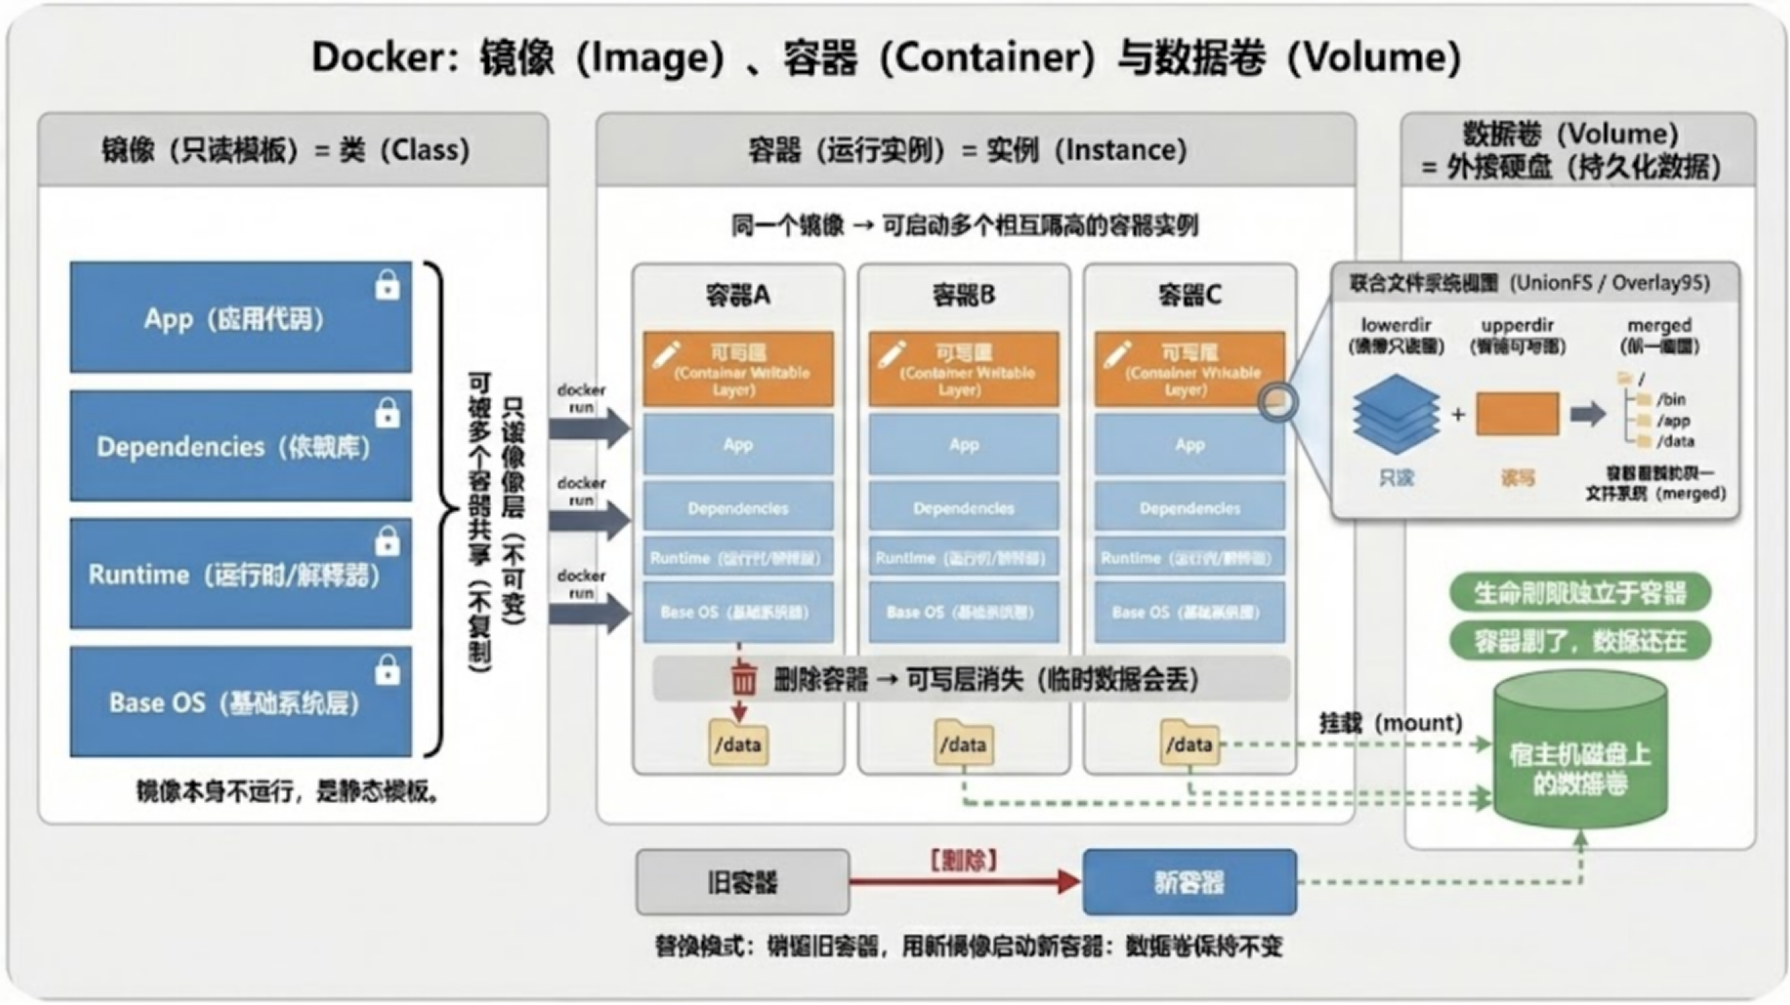
\includegraphics[width=1.0\textwidth]{figures/sec5/chapter5-2.png}
    \caption{镜像、容器以及数据卷}
    \label{fig:chapter5-2}
    \vspace{-15pt}
\end{figure*}


图 \ref{fig:chapter5-2}清晰地展示了 Docker 三大核心概念：镜像、容器与数据卷之间的逻辑关系与生命周期。在 Docker 的概念体系中，“镜像”与“容器”的关系就是图中所示的面向对象编程中的“类”与“实例”。如图左侧所示，镜像是静态的只读模板，它像一个被锁定的“千层饼”，将应用代码、依赖库及基础系统层自下而上封装在一起；而容器则是这个模板在特定宿主机上被“实例化”后的运行现场。正如图片中间部分所示，我们可以基于同一个只读镜像启动容器 A、B、C 等多个实例，它们就像用同一个类 new 出的多个对象，拥有独立的进程空间与网络环境，彼此隔离、互不干扰。这种架构让我们从传统的“修缮模式”彻底转变为图底部的“替换模式”：当应用需要更新时，我们不再修补旧容器，而是直接销毁它，并用新镜像启动新容器，从而保证了环境的绝对纯净。

从系统实现的角度看，容器之所以能做到秒级启动且占用极低，秘密藏在图 \ref{fig:chapter5-2} 中部的联合文件系统（UnionFS）放大视图中。容器并没有复制整个庞大的操作系统，而是采用了“分层复用”的机制：观察图中容器 A、B、C 的内部结构，你会发现它们底部都共享了蓝色的只读镜像层，Docker 仅仅是在这之上挂载了一层可写层。在容器运行期间，程序产生的所有状态变更，无论是写入日志、生成临时缓存，还是修改配置文件，实际上都发生在这个“顶层”里，而底下的镜像层始终保持只读不变。这种机制虽然高效，但也带来了一个必须警惕的副作用：可写层的生命周期是与容器绑定的。正如中下方的流程所示，一旦执行删除容器的操作，这层橙色的可写层也会随之灰飞烟灭，存储在其中的临时数据将永久丢失。

理解了“可写层即易失层”的本质，这就引出了一个棘手的工程问题：如果容器注定是“短命”的，那么像数据库文件、用户上传的图片这些长久的数据该存在哪里？为了解决这个问题，Docker 引入了图 \ref{fig:chapter5-2} 右侧所示的“数据卷（Volume）”。你可以将图中绿色的圆柱体想象成一块插在容器上的“外接硬盘”。通过挂载（mount）操作，我们打通了容器内部路径（如 /data）与宿主机磁盘之间的通道。当程序向这些路径写入数据时，数据流会直接穿透那层易失的橙色可写层，安全地落入宿主机的磁盘中。这样一来，计算逻辑（容器）与业务数据（卷）的生命周期就被彻底解耦了——哪怕你删除了容器、升级了镜像，只要挂载点不变，新启动的服务依然能无缝接管之前的数据，真正实现“铁打的数据，流水的容器”。


\subsubsection{分层构建：将“手工经验”转化为“显性指令”}\label{sec:dockerfile}

\begin{figure*}[htbp]
    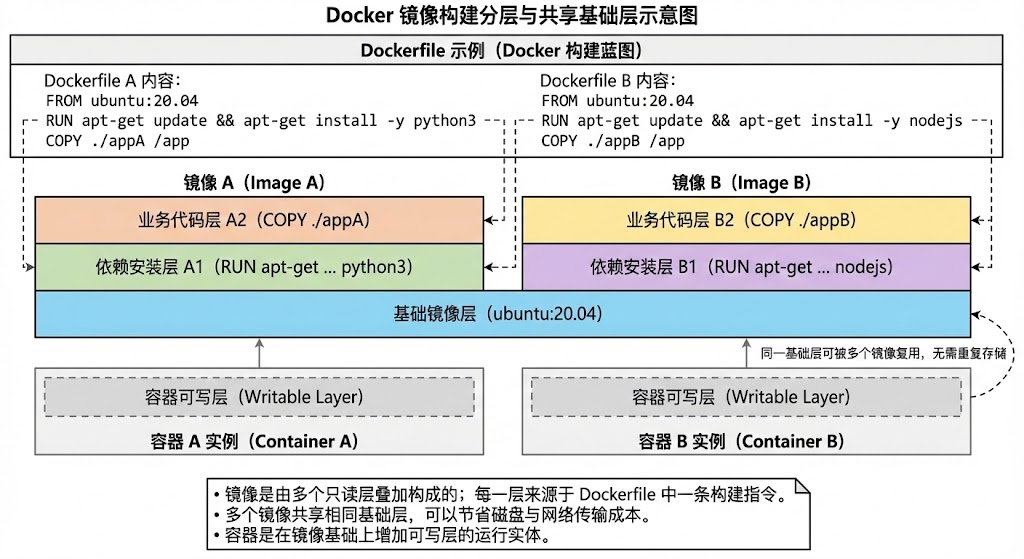
\includegraphics[width=1.0\textwidth]{figures/sec5/chapter5-1.png}
    \caption{Dockerfile构建镜像过程}
    \label{fig:chapter5-1}
    \vspace{-15pt}
\end{figure*}

如图 \ref{fig:chapter5-1} 展示了 Docker 镜像构建的分层机制与共享原理。要确保构建的细节，我们必须理解它是如何被“制造”出来的，Docker 镜像并非一个简单的压缩包，而是严格基于图顶部的 Dockerfile（构建蓝图）生成的。

这份文件充当了不可变的指令集，图中左侧的 Dockerfile A 与右侧的 Dockerfile B 清晰地演示了这一过程：每一行指令都对应一个构建步骤。无论是 FROM 定义的基础环境，还是 RUN 执行的软件安装（如 Python3 或 Node.js），当 Docker 执行这份文件时，会将每一条指令转化为镜像结构中一个独立的只读层。这些层并非混乱堆叠，而是严格按照指令顺序由下至上累积，每一层仅记录相对于上一层发生的增量变化。

这种“指令即图层”的设计在架构层面体现出了显著的优势，首当其冲的便是极致的资源复用。如图中部的蓝色区域所示，虽然镜像 A 与镜像 B 在上层的业务代码与依赖环境上各不相同，但它们均基于 ubuntu:20.04 这一共同的基座。在物理存储层面，这层基础镜像层无需重复冗余，只需存在一份即可被所有上层应用透明共享。这种机制意味着在部署大规模微服务时，系统仅需为各自业务代码（如 appA 或 appB）产生的差异部分“付费”，从而极大地降低了磁盘占用与网络传输的成本。

此外，该设计还实现了确定性与灵活性的完美共存。由于整个构建过程被完全代码化，只要 Dockerfile 保持不变，生成的镜像结构（Image A/B）在任何环境中都能保证分毫不差。如图底部所示当镜像真正投入运行时，Docker 仅需在原有的只读镜像层之上，动态加载一个容器可写层。这一精妙设计既通过只读层保证了底层环境的不可变性，又通过可写层赋予了容器实例必要的运行时读写权限，从而彻底将环境搭建转变为了一条高效、透明且可重复的自动化流水线。

Go 语言常被誉为“云原生时代的 C 语言”，其静态编译特性若能与 Docker 的分层构建机制深度结合，将产生极高的工程价值。纸上得来终觉浅，在上一章中，为了应对多人在线的负载压力，我们将游戏架构垂直拆解为了大厅服务与战斗服务两个独立模块；在本节中我们介绍了Docker的分层构建机制。然而，面对日益增多的服务组件以及未来潜在的水平扩容（如增开一区、二区），倘若机械地为每一个服务单独维护一份 Dockerfile，维护成本无疑将成倍攀升，为此接下来将演示如何编写一份通用的 Dockerfile。

\begin{tcolorbox}[title=拆分后的通用Dockerfile]
\begin{lstlisting}[
    language=bash,
    basicstyle=\ttfamily\footnotesize,
    numbers=left,                   % 开启左侧行号
    numberstyle=\tiny\color{gray},  % 行号样式：灰色小号字体
    numbersep=5pt,                  % 行号与代码的距离
    aboveskip=0pt, belowskip=0pt,
    lineskip=-1pt,
    commentstyle=\color{gray},
    keywordstyle=\color{blue}\bfseries,
    breaklines=true,
    showstringspaces=false
]
FROM golang:1.21-alpine AS builder # 编译环境 
WORKDIR /app # 在容器内的工作目录
COPY go.mod go.sum ./ # 复制关键Go工程文件
RUN go mod download # 下载依赖
COPY . .  # 将源码完整复制
ARG SERVICE # 需要构建的具体服务名
RUN if [ -z "$SERVICE" ]; then echo "ERR: SERVICE not set"; exit 1; fi
# 静态编译：生成的二进制统一命名为 server_bin
RUN CGO_ENABLED=0 GOOS=linux go build -o server_bin ./cmd/${SERVICE}
FROM alpine:latest # 生产环境
RUN apk --no-cache add ca-certificates tzdata # 防止时间偏差
WORKDIR /root/
# 仅从 Builder 阶段复制最终二进制产物与配置
COPY --from=builder /app/server_bin .
COPY --from=builder /app/config ./config
CMD ["./server_bin"]
\end{lstlisting}
\end{tcolorbox}

上面这份Dockerfile体现的核心，不是"命令怎么写"，而是如何把构建过程组织成可扩展、可复用、可缓存的工程系统。通过\textbf{多阶段构建}，我们把约300\,MB的Go工具链限制在构建阶段，把运行阶段收敛到约5\,MB的Alpine环境，最终镜像通常只有10--15\,MB。这意味着在游戏服务需要快速扩容时，节点拉取镜像的时间会显著缩短，发布与弹性伸缩的响应速度也会更高。

同时，Docker采用内容寻址存储（Content-Addressable Storage）机制，每个镜像层都由SHA256摘要唯一标识；当大厅服务与战斗服务共享基础层或依赖层时，仓库和宿主机只保存一份即可。这种按层去重机制会同时降低磁盘占用与网络传输开销，特别适合多服务并行演进的云原生系统。在缓存层面，先复制\texttt{go.mod}与\texttt{go.sum}可以稳定依赖层缓存，日常只改业务源码时通常只需重建最上层，本质上是在利用构建DAG的拓扑结构来最大化缓存命中率。关于这份 Dockerfile 每一行指令的详细解读，请参见附录C.2。

\subsubsection{隔离机制：进程的轻量级虚拟化}

根据上面的描述，我们应该可以发现容器能像虚拟机一样运行服务，但是为什么云计算会使用容器而不是虚拟机？根本原因是它具备业界认可的更轻量？在 图 \ref{fig:chapter5-3} 的宏观对比中，在左侧的传统虚拟机（VM）架构中每一台虚拟机不仅包含应用本身，还必须扛起一套沉重的客体操作系统（Guest OS）与模拟硬件层。这就像为了安顿一位远房亲戚，你得先建造一整栋独立的房子，开销自然极其巨大。反观图示中间的“Docker 容器”架构，你会发现那一层厚重的模拟硬件层和操作系统彻底消失了，取而代之的是所有容器直接坐落在“共享核心内核”之上。这种“进程级隔离”意味着容器不再重复启动内核，省去了漫长的开机自检与繁重的内存损耗，从而实现了“毫秒级启动”与极低资源开销。


那么Docker 是如何让这些共享内核的进程“感觉”自己是在独立运行的呢？答案藏在 图 \ref{fig:chapter5-3} 的右侧面板中，Linux 内核通过两大关键技术为进程构建了隐形的围墙。首先是图右上方的 Namespaces（命名空间），它就像是给进程戴上了一副“特制眼镜”，在 PID（进程号）、NET（网络栈）、MNT（文件挂载点）等维度上构建了独立的视图边界；在容器内部，进程只能看到自己的进程列表和网络接口，完全感知不到宿主机上其他进程的存在。与此同时，图右下方的 Cgroups（控制组） 则扮演了“配额管理员”的角色，它直接对接宿主机的资源池，严格限制了每个容器最多能消耗多少 CPU 时间片和内存大小，防止单个服务因资源失控而将整个服务器拖垮。

\begin{figure*}[htbp]
    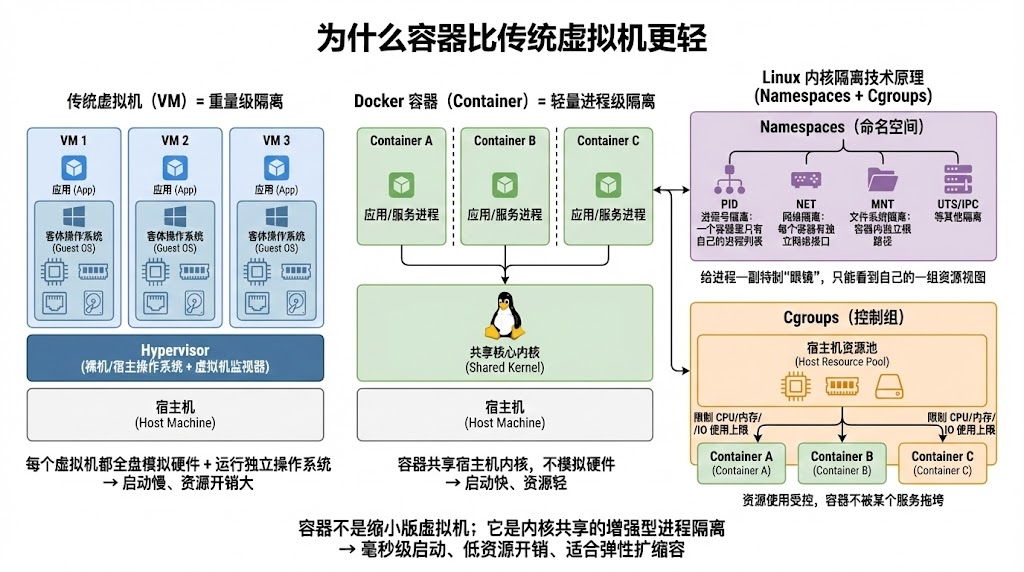
\includegraphics[width=1.0\textwidth]{figures/sec5/chapter5-3.png}
    \caption{容器与虚拟机的对比}
    \label{fig:chapter5-3}
    \vspace{-15pt}
\end{figure*}

理解了这张图的深层逻辑，我们就能建立起对容器最准确的直觉：容器绝不是一个“缩小版的虚拟机”，它的本质是一个“自带隔离边界的增强型进程”。 正是这种“共享内核”与“独占边界”的辩证统一，让 Docker 在保留了隔离安全性的同时，将资源利用率推向了极致。这不仅解释了为何它比虚拟机启动更快，更揭示了它为何能成为微服务架构下实现高频弹性扩缩容的技术基石。

不过，Namespace和Cgroups只是隔离的"骨架"，容器的网络通信还需要额外的机制来支撑。Docker启动一个容器时，会把它放进独立的Network Namespace里，容器内部看到的是自己的一组网络设备、IP地址、路由表以及\texttt{iptables}规则。因此，同一台主机上的不同容器即使并行运行，也不会天然共享网络配置，应用进程只会感知到所在命名空间的网络视图。从实现机制看，Docker通常会为容器创建一对\texttt{veth}虚拟网卡，它们像一根"虚拟网线"的两端：一端被放入容器的网络命名空间，作为容器内的网络出口；另一端留在宿主机侧，通常接入\texttt{docker0}网桥——可以理解为主机上的一个二层虚拟交换设备。当多个容器部署在同一宿主机时，\texttt{docker0}负责把这些容器端口连接起来。在同主机场景下，一个容器发出的数据包会先经过本容器的\texttt{veth}端口进入网桥，再由网桥转发到目标容器对应的\texttt{veth}端口，最终到达目标进程。

需要强调的是，容器与虚拟机在隔离强度上并不等价：容器共享宿主机内核，启动快、开销小，但内核攻击面的隔离相对更弱；虚拟机则为每个实例提供独立内核，边界更强，但资源成本与启动时延通常更高。因此在多租户云环境中，常见做法是引入gVisor、Kata Containers一类"轻量虚机化"方案，在性能与隔离之间取得折中。更深入的隔离原理（gVisor、Kata Containers等）将在第六章讨论。值得一提的是，上述\texttt{docker0}网桥模型是Docker默认的单机网络方案；进入Kubernetes之后，集群网络通常由CNI（Container Network Interface）插件接管，采用扁平化的跨节点组网方式，不再依赖\texttt{docker0}——这一点我们在后续K8s部分会自然感受到。


\subsubsection{交付闭环：分发与版本锁定}

\begin{figure*}[htbp]
    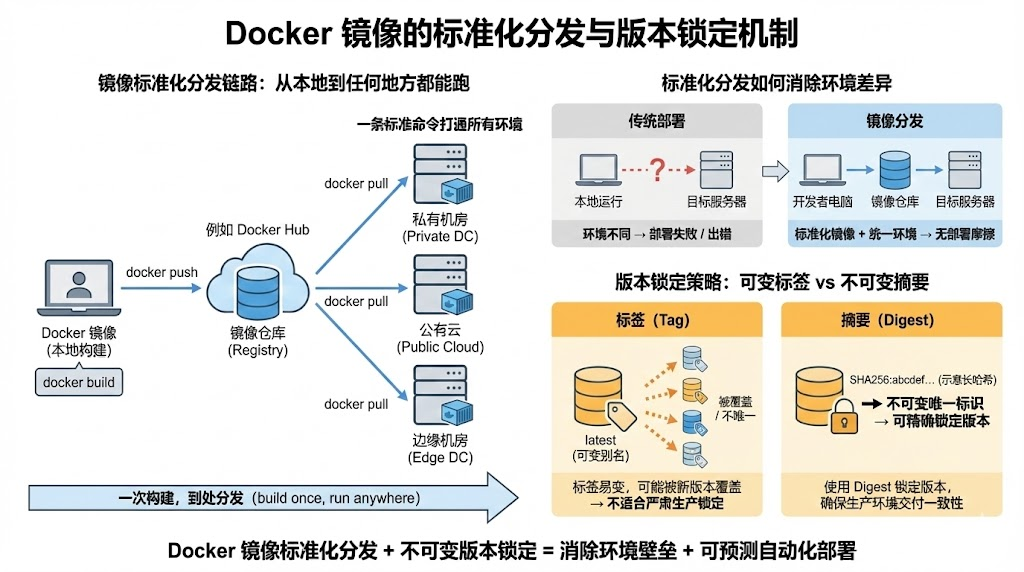
\includegraphics[width=1.0\textwidth]{figures/sec5/chapter5-4.png}
    \caption{Docker的标准化分发链路}
    \label{fig:chapter5-4}
    \vspace{-15pt}
\end{figure*}

Docker 之所以能将“我电脑上能跑”的单点偶然，转化为“处处能跑”的工程必然，其核心不仅取决于容器运行时的隔离性，更依赖于图 \ref{fig:chapter5-4} 所示的标准化分发链路。正如左侧主流程所示，镜像构建完成后，并非孤立存在于开发者的本地机器，而是通过 \texttt{docker push} 指令被推送到远端的镜像仓库（Registry），例如业界通用的 Docker Hub\footnote{Docker Hub: \url{https://hub.docker.com}}。这一机制构建了一个中心化的“软件物流中心”，彻底打通了开发环境与生产环境之间的物理壁垒：无论目标服务器是位于私有机房、公有云还是边缘节点，只要网络连通，运维人员只需执行 \texttt{docker pull} 指令，即可将包含完整运行环境的交付物原样拉取下来。这种“中间库”模式消除了传统部署中点对点拷贝代码导致的“环境摩擦”，真正实现了从“本地运行”到“一次构建，四处分发”的跨越。

为了确保生产环境的绝对严谨，业界在分发环节通常会执行更严格的版本锁定策略，这一关键区别清晰地展示在图 \ref{fig:chapter5-4} 右下角的细节中。虽然 Docker 提供了 \texttt{latest} 等标签（Tag）机制，但标签本质上是可变的别名，极易被新推送的版本覆盖，导致不同时间拉取的 \texttt{latest} 实际上是完全不同的代码。因此，在工程实践中，我们更倾向于使用镜像摘要（Digest）——即对镜像内容进行 SHA256 哈希计算生成的唯一且不可变的标识符——来锁定版本。这标志着软件交付模式的根本性变革：我们将交付过程从传统的“拷贝代码 + 祈祷不报错”，进化为“拉取标准化构件 + 校验唯一哈希 + 按约定启动”。这种基于密码学保证的一致性，使得规模化的自动化部署不再是碰运气的冒险，而是可预测的工程行为。

理论为我们指明了方向，而终端命令则是走完这“发布最后一公里”的具体载体。当我们的战斗服业务代码编写完毕，并按照 \ref{sec:dockerfile} 节的要求定义好 Dockerfile 后，整个交付流水线便正式启动：首先，使用 \texttt{docker build} 命令配合 \texttt{-t} 参数构建出带有版本号的本地镜像；紧接着，通过 \texttt{docker login} 指令与 Docker Hub 或私有仓库建立加密的安全连接，完成身份认证；随后，利用 \texttt{docker tag} 给本地镜像打上带有云端用户名的“发件人标签”，确保其能被准确路由至指定仓库；最后，执行 \texttt{docker push} 将镜像推向云端。在此过程中，Docker 的智能分层机制会确保只上传云端缺失的增量层，极大节省带宽，而推送结束时返回的那串 SHA256 摘要，正是我们在后续 \texttt{pull} 指令中进行精确版本锁定的唯一凭证。

\begin{tcolorbox}[title=镜像发布与版本锁定实操]
\begin{lstlisting}[
    language=bash,
    basicstyle=\ttfamily\footnotesize,
    numbers=left,                   % 开启左侧行号
    numberstyle=\tiny\color{gray},  % 行号样式：灰色小号字体
    numbersep=5pt,                  % 行号与代码的距离
    aboveskip=0pt, belowskip=0pt,
    lineskip=-1pt,
    commentstyle=\color{gray},
    keywordstyle=\color{blue}\bfseries,
    breaklines=true,
    showstringspaces=false
]
docker build -t game-lobby:v1 . # 构建镜像
docker login # 登录镜像仓库
docker tag game-lobby:v1 username/game-lobby:v1 # 打标签
docker push username/game-lobby:v1 # 推送到云端
docker pull username/game-lobby@sha256:[sha256] # 从云端拉取
docker images --digests # 验证镜像是否一致 
\end{lstlisting}
\end{tcolorbox}


然而，掌握了单个容器的标准化交付仅仅是构建云原生架构的起点。现实中的现代应用，尤其是复杂的分布式游戏后端，往往是由多个相互依赖的服务（如游戏服、数据库、缓存、网关）共同构成的有机体。在下一节，我们将把视角从“单机容器”扩展至“集群编排”：利用 Docker Compose 解决多服务协同与本地联调的难题。



\subsection{一键开服：使用 Compose 编排你的游戏``大区''}

\subsubsection{从手工拼装到一键编排}

上一节我们学会了如何将单个游戏服务封装成 Docker 容器，但现实中的游戏后端远不止一个孤立的服务。回想第四章构建的分布式架构，我们至少有玩家接入的网关服务、负责战斗计算的地图服务、存储玩家数据的 Redis 缓存，以及记录操作日志的数据库服务。要让“游戏大区”真正运行起来，必须协调启动多个容器，并保证它们之间的启动顺序、网络连接和配置传递正确无误。

如果依赖手工操作，流程会变得极为繁琐，甚至痛苦。比如以 Bash 命令为例，你可能需要这样逐步执行：

\begin{tcolorbox}[title=手工操作]
\begin{lstlisting}[
    language=bash,
    basicstyle=\ttfamily\footnotesize,
    numbers=left,                   % 开启左侧行号
    numberstyle=\tiny\color{gray},  % 行号样式：灰色小号字体
    numbersep=5pt,                  % 行号与代码的距离
    aboveskip=0pt, belowskip=0pt,
    lineskip=-1pt,
    commentstyle=\color{gray},
    keywordstyle=\color{blue}\bfseries,
    breaklines=true,
    showstringspaces=false
]
# Step 1: 启动数据库容器，确保其先就绪
docker run -d --name mysql-db -e MYSQL_ROOT_PASSWORD=123456 mysql

# Step 2: 启动 Redis 缓存（依赖数据库）
docker run -d --name redis-cache redis

# Step 3: 启动地图服务容器，配置数据库连接地址
docker run -d --name map-service --link mysql-db:mysql -p 8081:8080 game/map-service

# Step 4: 启动网关服务容器，连接地图服务
docker run -d --name gateway-service --link map-service:map -p 8080:8080 game/gateway

# 还需确保端口不冲突、网络互通，每次启动都要验证服务健康
\end{lstlisting}
\end{tcolorbox}

从上面可以看到，启动五个相关联的服务不仅命令多且复杂，必须严格按照顺序执行，稍有疏忽就可能导致连接失败或服务不可用。每次发布、每次更新都要重复执行这套“开机仪式”，运维成了折磨人的手工活。

Docker Compose 的出现极大地简化了这一切。如图 \ref{fig:compose-concepts} 所示，它通过一份声明式的配置文件，清晰描述了所有服务的镜像、端口映射、环境变量、依赖关系以及网络设置。只需一条命令：

\begin{tcolorbox}[title=Docker Compose]
\begin{lstlisting}[
    language=bash,
    basicstyle=\ttfamily\footnotesize,
    numbers=left,                   % 开启左侧行号
    numberstyle=\tiny\color{gray},  % 行号样式：灰色小号字体
    numbersep=5pt,                  % 行号与代码的距离
    aboveskip=0pt, belowskip=0pt,
    lineskip=-1pt,
    commentstyle=\color{gray},
    keywordstyle=\color{blue}\bfseries,
    breaklines=true,
    showstringspaces=false
]
docker-compose up -d
\end{lstlisting}
\end{tcolorbox}

Docker Compose 会自动解析依赖关系，按正确顺序启动服务，并创建默认网络保证容器间通信。部署效率大幅提升，省去了重复的手工操作和配置错误的风险。

更重要的是，随着游戏规模扩大，实际生产环境的容器数量可能从几个增加到几十、几百，涵盖多个微服务、缓存、数据库、消息队列等组件。此时依赖手工启动根本无法胜任。Docker Compose 通过集中管理和自动编排，成为中小型多容器应用的理想选择，帮助开发者和运维人员提升效率、降低出错率。

\begin{figure}[htbp]
\centering

\includegraphics[width=0.85\textwidth]{figures/sec5/Docker_Compose_concepts.png}
\caption{Docker Compose 服务编排的核心概念与工作机制}
\label{fig:compose-concepts}
\end{figure}

总之，从“手工拼装”到“一键编排”，Docker Compose 帮助我们将复杂的容器启动流程变成规范、可复用的标准操作，为游戏大区的稳定运行提供了坚实保障。

\subsubsection{理解 Docker Compose：从“单兵作战”到“团队协作”}

Docker Compose 是专门为多容器应用设计的编排工具，它通过 YAML 格式的配置文件，定义和管理一组相关服务的运行环境。如果说 Docker 解决了“如何标准化打包和运行单个服务”的问题，那么 Compose 解决的则是“如何让多个服务协调工作、组成完整系统”的问题。

可以把 Compose 想象成一位交响乐团的指挥家。每个容器就像一个乐器，单独演奏可能不错，但要奏出和谐动人的乐章，就需要指挥家协调各个乐器的节奏、开合与配合。Compose 通过声明式的配置文件，让我们只需描述“想要什么样的整体效果”（即哪些服务需要运行、它们之间如何连接交流），而不用关心“具体如何实现”（启动顺序、网络配置等琐细）。

这种抽象带来了极大的便利和价值：无论是在开发机、测试环境还是生产集群，使用同一份 Compose 配置文件，都能确保部署一致、不出差错，也方便维护和升级。新增服务或更改配置，只需更新配置文件即可，让复杂分布式应用的管理变得简单、高效。

下面示例展示了一个典型的 Docker Compose 配置，用于定义一个包含数据库、缓存、地图服务和网关服务的游戏后端应用：

\begin{tcolorbox}[title=Docker Compose 配置示例]
\begin{lstlisting}[
    language=bash,
    basicstyle=\ttfamily\footnotesize,
    numbers=left,                   % 开启左侧行号
    numberstyle=\tiny\color{gray},  % 行号样式：灰色小号字体
    numbersep=5pt,                  % 行号与代码的距离
    aboveskip=0pt, belowskip=0pt,
    lineskip=-1pt,
    commentstyle=\color{gray},
    keywordstyle=\color{blue}\bfseries,
    breaklines=true,
    showstringspaces=false
]
version: "3"
services:
  mysql-db:
    image: mysql:5.7
    environment:
      MYSQL_ROOT_PASSWORD: "123456"
    ports:
      - "3306:3306"
    volumes:
      - db-data:/var/lib/mysql

  redis-cache:
    image: redis:6
    ports:
      - "6379:6379"

  map-service:
    image: game/map-service:v1
    depends_on:
      - mysql-db
      - redis-cache
    ports:
      - "8081:8080"
    environment:
      DB_HOST: mysql-db
      REDIS_HOST: redis-cache

  gateway-service:
    image: game/gateway:v1
    depends_on:
      - map-service
    ports:
      - "8080:8080"
    environment:
      MAP_SERVICE_HOST: map-service

volumes:
  db-data:
\end{lstlisting}
\end{tcolorbox}

这段配置清楚列出了四个服务及其相关属性：\texttt{mysql-db} 和 \texttt{redis-cache} 分别是数据库和缓存服务，定义了镜像、端口映射及持久化存储策略。\texttt{map-service} 依赖数据库和缓存，配置了端口以及环境变量指向依赖服务的容器名。\texttt{gateway-service} 依赖地图服务，配置相应端口和环境变量。

当执行 \texttt{docker-compose up} 命令时，Compose 会根据 \texttt{depends\_on} 关系自动控制启动顺序，确保各个容器按需启动并建立网络连接，无需我们编写繁琐的启动脚本。

这样的声明式结构，极大提升了多容器应用的可维护性和可移植性，减少了因环境差异或人为操作失误带来的风险。对于日益复杂的游戏后端多服务体系，Docker Compose 是开发和运维人员的得力助手。

紧接着这一点，Compose 的声明式配置还带来一个非常关键的特性：幂等性。开发者反复执行 \texttt{docker-compose up} 时，系统目标状态并不会被"叠加执行"，而是由 Compose 先比对当前状态与配置文件中的期望状态，再只进行必要的创建、重建或更新操作。相比之下，命令式脚本如果被重复运行，常常会出现重复容器、端口占用冲突等问题，排障成本很高。也正因为如此，Compose 文件本身就成为唯一可信的事实来源，这正是基础设施即代码在工程实践中的核心价值。

\subsubsection{Docker Compose 的工作机制：配置如何变成运行的服务}

理解了 Docker Compose 的配置文件后，一个自然的问题是：当我们执行 \texttt{docker-compose up} 命令时，背后究竟发生了什么？这份看似简单的 YAML 配置是如何转化为实际运行的容器集群的？

Docker Compose 的工作流程可以分为四个核心阶段，每个阶段都体现了自动化编排的智能之处。理解这个过程，能帮助我们更好地诊断问题、优化配置，也能让我们对容器编排有更深刻的认识。

当你执行 \texttt{docker-compose up} 命令时，Compose 首先会读取当前目录下的配置文件，并对其进行语法验证和语义分析。这个过程就像建筑师审阅施工图纸，检查是否有不合理或矛盾的设计。之后，Compose 会根据配置中的 \texttt{depends\_on} 字段构建服务之间的依赖关系图。在我们的游戏后端示例中，网关服务依赖地图服务，地图服务依赖数据库和缓存，这形成了一个有向无环图（DAG）。Compose 会对这个图进行拓扑排序，确定各个服务的启动顺序，保证被依赖的服务总是先于依赖它的服务启动。

这种智能分析避免了手动管理启动顺序的麻烦。想象如果手工操作，你需要记住"必须先启动数据库，等它就绪后再启动地图服务"这样的规则，而且随着服务数量增加，这种依赖关系会变得极其复杂。Compose 自动处理这一切，让我们只需声明依赖关系，具体执行交给工具。

为了解决容器互联的问题，Compose 会在启动任何容器之前首先创建一个专属的虚拟网络。默认情况下，这个网络使用项目名称（通常是配置文件所在目录的名字）作为前缀命名。这个网络相当于为所有服务提供了一个隔离的通信空间，就像为乐团成员准备了一个专门的排练厅。网络创建完成后，Compose 还会为每个服务配置 DNS 解析。这是一个非常巧妙的设计：在这个虚拟网络中，每个容器都可以通过服务名直接访问其他容器，而不需要知道具体的 IP 地址。例如，地图服务的代码中可以直接使用 \texttt{mysql-db} 这个主机名连接数据库，Compose 会自动将其解析为数据库容器的实际 IP 地址。

这种服务发现机制极大简化了服务间通信的配置。传统方式下，你需要手动管理每个服务的 IP 地址，当容器重启导致 IP 变化时，还要更新所有相关的配置。而使用 Compose，这一切都是自动的，容器之间通过稳定的服务名通信，底层 IP 变化完全透明。

网络就绪后，Compose 开始根据依赖顺序启动容器。这个过程遵循严格的拓扑顺序：先启动没有依赖的基础服务（如数据库和缓存），等它们成功运行后，再启动依赖它们的中间层服务（如地图服务），最后启动最上层的服务（如网关）。

对于每个服务，Compose 会执行以下操作：首先检查本地是否已有对应的镜像，如果没有则自动从镜像仓库拉取；然后根据配置创建容器，包括设置环境变量、挂载数据卷、映射端口等；最后将容器加入之前创建的虚拟网络，并启动容器进程。这里有一个重要的细节需要注意：\texttt{depends\_on} 只保证容器的启动顺序，并不等待服务真正就绪。例如，即使数据库容器已经启动，数据库服务本身可能还在初始化过程中，尚未准备好接受连接。对于这种情况，应用代码需要实现重试逻辑，或者使用健康检查机制来确保依赖服务真正可用后再启动。

在依赖就绪不可完全由 \texttt{depends\_on} 保证之后，重启策略就是提升稳定性的下一道防线。对于需要长期运行的游戏后端服务，Compose 提供的 \texttt{restart: always}、\texttt{on-failure}、\texttt{unless-stopped} 各有语义：\texttt{always} 表示无论何种退出都自动拉起，\texttt{on-failure} 只在非零退出码时重启，更适合避免误重启，\texttt{unless-stopped} 则会尊重人工停机操作。它们虽然简单，却已经体现出自愈机制的雏形。后续学习 Kubernetes 时，你会看到同类能力被扩展为更细致的 Pod 重启策略与跨节点重新调度。

所有服务启动完成后，Compose 并不是简单地退出，而是持续监控各个容器的运行状态。如果某个容器异常退出，Compose 会根据配置决定是否自动重启。默认情况下，Compose 会聚合所有容器的日志输出，并标注服务名称，方便我们统一查看和调试。

这种集中式的日志管理在多容器环境下尤其有价值。传统方式下，你需要逐个登录到每个容器查看日志，非常低效。而使用 Compose，只需执行 \texttt{docker-compose logs} 命令，就能看到所有服务的日志输出，还可以通过 \texttt{-f} 参数实时跟踪，或通过服务名过滤特定服务的日志。

\begin{figure}[htbp]
\centering
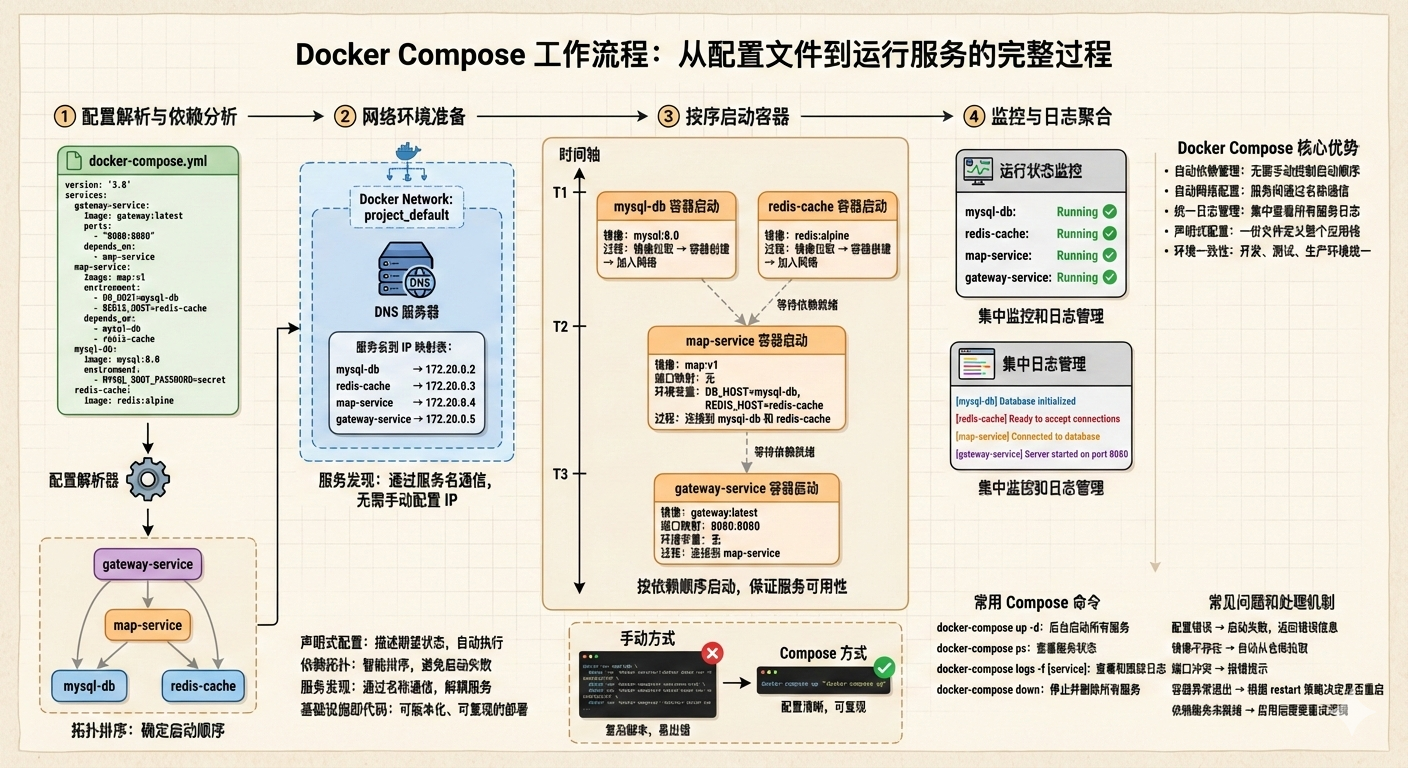
\includegraphics[width=0.9\textwidth]{figures/sec5/docker-compose-workflow.png}
\caption{Docker Compose 工作流程：从配置文件到运行服务的完整过程}
\label{fig:compose-workflow}
\end{figure}

如图 \ref{fig:compose-workflow} 所示，整个工作流程是一个高度自动化的过程，从配置解析到服务运行，每个环节都经过精心设计。Compose 将复杂的多容器编排抽象为简单的配置管理，让开发者可以专注于应用逻辑，而不是被部署细节所困扰。

需要特别强调的是，Docker Compose 的这种工作方式体现了"基础设施即代码"的理念。整个应用的部署拓扑、网络配置、环境参数都以代码形式保存在配置文件中，可以版本控制、可以审查、可以复现。这种标准化的部署方式，是现代软件工程从手工作坊向工业化生产转变的重要标志。

当然，Docker Compose 主要适用于单机或小规模的多容器部署场景。当应用规模扩展到需要跨多台机器、需要更复杂的调度策略和故障恢复机制时，就需要使用更强大的编排工具，比如我们即将学习的 K8s。但无论如何，理解 Compose 的工作机制，都是掌握容器编排技术的重要基础。

但当项目从几百名在线玩家增长到上千甚至更多时，Compose 的边界会很快显现。它本质上依赖单一 Docker Engine，所有容器通常集中在一台机器上运行，这意味着一旦主机发生硬件故障，服务整体可用性会受到直接冲击。由于缺乏跨节点调度能力，Compose 不能把负载自动分散到多台服务器，也无法在节点失效后把工作负载迁移到健康节点。发布层面上，它也不具备真正的滚动更新机制，常见做法是重建容器，这在在线游戏场景中容易引入可感知中断。扩缩容方面，Compose 缺少面向实时负载的自动伸缩控制，难以应对活动高峰时的突发流量。于是，团队会自然转向 Kubernetes：把多机集群调度、滚动发布、故障恢复与弹性伸缩统一纳入同一套编排体系，这也是从开发便利走向生产级治理的关键一步。

%\subsection{踏上云端：从本地上云}
%\paragraph{本节目标} 理解上云本质，掌握 “选服务器 - 传镜像 - 启动服务” 流程。
%\paragraph{写作建议} 
%\begin{enumerate}
%    \item 列上云优势：性能弹性、公网访问、宕机重启。
%    \item  分 3 步：选带 Docker 的云服务器、传镜像（仓库下载 / 直接拷贝）、启动服务 + 开安全组端口。
%\end{enumerate}

\subsection{从物理机到云端：理解虚拟化与云计算}

在前两节中，我们用Docker解决了环境一致性问题，用Compose实现了多服务的本地编排。但这一切仍然运行在我们自己的电脑上——一台摆在桌上的、随时可能断电的物理机器。要让游戏世界真正面向玩家开放，我们必须把服务搬到云端。然而，"上云"并不只是"换个地方跑程序"这么简单。在动手操作之前，我们需要先理解一个根本性的问题：云服务器到底是什么？它和我们面前的这台电脑有什么本质区别？

\subsubsection{物理机与云主机：真实硬件与虚拟切片}

我们日常使用的个人电脑或机房里的服务器，都是\textbf{物理机}（Physical Machine）。它拥有真实的CPU芯片、内存条、硬盘和网卡，所有计算资源都由这一台机器独占。当我们在物理机上安装Docker并运行游戏服务器时，容器直接共享宿主机的Linux内核，性能损耗极小——这也是第一节中Docker能做到"秒级启动"的根本原因。

而当我们在阿里云、腾讯云或AWS上"购买一台服务器"时，我们拿到的并不是一台真实的物理机器，而是一台\textbf{云主机}（Cloud Virtual Machine）。云主机的本质是一个运行在大型物理服务器上的\textbf{虚拟机}（Virtual Machine, VM）。一台配备了128核CPU和512GB内存的物理服务器，可以被切分成几十台小规格的云主机，分别租给不同的用户。你在云控制台上看到的"2核4GB"实例，实际上只是这台庞大物理机上的一个"切片"。

这就引出了一个有趣的问题：如果云主机本身已经是虚拟化的产物，那么在云主机里再运行Docker容器，岂不是"虚拟化之上再虚拟化"？这种\textbf{嵌套虚拟化}（Nested Virtualization）确实存在。好消息是，Docker容器并不是传统意义上的虚拟机——正如第一节所讲，容器只是一个被Namespace和Cgroups隔离的进程，它直接使用宿主机（即云主机）的内核，并不需要模拟硬件。因此，在绝大多数云主机上运行Docker是完全可行的，性能损耗也在可接受范围内。但在某些特殊的云环境中（例如某些轻量级容器实例服务），由于底层已经使用了容器技术来隔离租户，再在其中运行Docker可能会遇到权限限制或兼容性问题。理解这一点，能帮助你在遇到"Docker在云上跑不起来"的问题时快速定位原因。

\subsubsection{虚拟化的本质：一台机器如何变成多台}

既然云主机是虚拟化的产物，那虚拟化到底是怎么实现的？其核心在于一个叫做\textbf{Hypervisor}（虚拟机监控器，也称VMM）的软件层。Hypervisor的职责是在一台物理机上创建并管理多个虚拟机，让每个虚拟机都"以为"自己独占了整台硬件。

根据Hypervisor的运行位置，业界将其分为两种类型。\textbf{Type-1 Hypervisor}（裸金属型）直接运行在物理硬件之上，不需要宿主操作系统。典型代表包括Linux内核中的\textbf{KVM}（Kernel-based Virtual Machine）和VMware的\textbf{ESXi}。主流云厂商几乎都采用这种方案，因为它省去了宿主操作系统的开销，能够将更多的硬件资源分配给虚拟机。\textbf{Type-2 Hypervisor}（宿主型）则运行在一个普通操作系统之上，就像一个普通的应用程序。我们在个人电脑上使用的\textbf{VirtualBox}和VMware Workstation就属于这一类。它的优势是安装简单、便于开发测试，但由于多了一层宿主操作系统的开销，性能不如Type-1。

从更宏观的视角看，虚拟化技术实现了\textbf{资源池化}（Resource Pooling）——将一台物理机的CPU、内存、存储和网络资源抽象为一个"资源池"，然后按需切分给不同的虚拟机。这就好比一栋大楼被分隔成多个独立的办公室出租：每个租户拥有自己的门锁和空间，互不干扰，但底层的电力、网络和消防系统是共享的。对于我们的游戏服务器来说，我们租用的那台"2核4GB"云主机，就是从一台强大的物理服务器的资源池中切分出来的一小块。

\subsubsection{云计算的三层抽象：IaaS、PaaS与SaaS}

理解了虚拟化之后，我们可以进一步认识云计算的全貌。云计算并不是单一的技术，而是一套分层的服务体系。根据云厂商为用户屏蔽了多少底层复杂性，业界将云服务划分为三个经典层次。

\begin{table}[htbp]
\centering
\begin{tabular}{|l|l|l|l|}
\hline
\textbf{层次} & \textbf{全称} & \textbf{用户管理} & \textbf{典型产品} \\
\hline
\textbf{IaaS} & 基础设施即服务 & OS、运行时、应用 & 阿里云ECS、AWS EC2 \\
\hline
\textbf{PaaS} & 平台即服务 & 应用代码与数据 & 阿里云ACK、Google GKE \\
\hline
\textbf{SaaS} & 软件即服务 & 仅使用，无需管理 & Gmail、钉钉、腾讯文档 \\
\hline
\end{tabular}
\caption{云计算三层服务模型对比}
\label{tab:cloud-service-layers}
\end{table}

\textbf{IaaS}（Infrastructure as a Service，基础设施即服务）是最底层的云服务。云厂商提供虚拟机、网络和存储等基础资源，用户需要自己安装操作系统、配置环境、部署应用。我们在前面讨论的"租一台云服务器，装上Docker，跑游戏服务"就是典型的IaaS使用方式。用户拥有最大的自由度，但也承担了最多的运维责任。

\textbf{PaaS}（Platform as a Service，平台即服务）在IaaS之上又屏蔽了一层。云厂商不仅提供基础设施，还提供了运行时环境、中间件和开发工具。用户只需要关心自己的应用代码和数据，不需要操心操作系统的补丁更新、运行时的版本管理等问题。我们即将在下一节学习的Kubernetes托管服务（如阿里云ACK、Google GKE）就属于PaaS——云厂商帮你管理K8s集群的控制平面，你只需要提交Deployment配置，集群的维护和升级由平台负责。

\textbf{SaaS}（Software as a Service，软件即服务）是抽象程度最高的层次。用户直接使用现成的软件产品，完全不需要关心底层的任何技术细节。我们日常使用的电子邮件、在线文档、即时通讯工具都属于SaaS。

那么我们的游戏服务器处于哪一层？答案取决于我们的部署方式。当我们直接租用云主机、手动安装Docker并部署服务时，我们使用的是IaaS；当我们使用云厂商提供的K8s托管服务时，我们就升级到了PaaS层。云原生技术的演进方向，正是不断将开发者从底层运维中解放出来，让他们能够把更多精力投入到游戏逻辑本身。

\subsubsection{网络虚拟化：云上的私有局域网}

除了计算资源的虚拟化，云端还有一个容易被忽视但至关重要的概念：\textbf{网络虚拟化}。在传统的物理机房中，服务器之间通过交换机和路由器组成局域网，网络拓扑是物理的、可见的。但在云端，成千上万台虚拟机共享同一套物理网络基础设施，如何保证不同租户之间的网络隔离？

云厂商通过\textbf{VPC}（Virtual Private Cloud，虚拟私有云）来解决这个问题。VPC本质上是在云端为你划出的一块"私有局域网"。你可以在VPC内自由规划子网、分配IP地址、设置路由规则，就像在自己的机房里搭建网络一样。不同VPC之间默认是完全隔离的，即使两个VPC中的虚拟机恰好运行在同一台物理服务器上，它们也无法互相访问。

在VPC的基础上，云厂商还提供了\textbf{安全组}（Security Group）机制来实现精细化的访问控制。安全组遵循\textbf{"默认拒绝，显式允许"}的原则：新创建的云主机默认拒绝所有入站流量，你必须手动添加规则来开放特定端口。对于我们的游戏服务器，至少需要开放游戏客户端连接的端口（如WebSocket的9090端口）和HTTP接口端口（如8080端口），同时将数据库端口（如MySQL的3306端口）限制为仅允许同一VPC内的服务器访问，绝不对公网开放。

理解了VPC和安全组的概念，你就掌握了云端网络配置的核心逻辑。具体的云端部署操作步骤——包括如何选择云服务器、迁移Docker镜像、配置安全组规则以及进行端到端测试——请参见附录C。


%\subsection{云端指挥官：Kubernetes 容器编排入门}
%\paragraph{本节目标} 理解 K8s 作用，掌握核心概念与部署流程。
%\paragraph{写作建议}
%\begin{enumerate}
%    \item 以 “多机管 多个容器麻烦” 痛点，引出 K8s（统一管多机容器）。
%    \item 讲核心概念：Pod（最小单元）、Deployment（管 Pod）、Service（分发请求）、Node（云服务器）。
%    \item 提部署流程：传镜像、写配置文件、执行命令创建 Deployment/Service。
%\end{enumerate}

\subsection{云端指挥官：Kubernetes 容器编排入门}

\subsubsection{从单机到集群：当容器多到管不过来}

在上一节中，我们成功地将游戏服务部署到了单台云服务器上，这标志着从本地开发向云端运行的重要跨越。然而，随着游戏用户量的增长和业务复杂度的提升，单台服务器很快就会遇到新的瓶颈。想象一下这样的场景：你的游戏突然火爆，同时在线人数从几百人暴涨到几万人，单台服务器开始不堪重负，响应时间急剧恶化。此时你急需增加更多服务器来分担压力，但面临的却是一个令人头疼的管理难题。

这种困境的核心问题在于"规模化管理的复杂性爆炸"。当你只有一台服务器时，管理工作相对简单：登录服务器、检查服务状态、重启容器、查看日志。但当服务器数量增加到10台、50台、100台时，这种一对一的管理方式就完全不可持续了。你需要记住每台服务器的IP地址、监控每台机器的资源使用情况、手动协调服务器之间的负载分配，更要命的是，当某台服务器宕机时，你需要手动将其承载的服务迁移到其他服务器上。

传统的扩展方式需要你手动购买更多云服务器，然后在每台机器上重复相同的部署流程：安装Docker、配置环境、拉取镜像、启动容器、配置网络。这个过程不仅耗时费力，更容易出错。即使你编写了自动化脚本，也很难处理各种异常情况：网络故障导致镜像拉取失败、资源不足导致容器启动失败、配置差异导致服务行为不一致等等。

更深层的问题是缺乏统一的协调机制。多台服务器独立运行时，它们互不了解彼此的状态，无法进行智能的负载分配和故障转移。当某台服务器过载时，新的请求仍然可能被分配到它上面；当某台服务器宕机时，其他服务器无法自动接管其工作负载。这种各自为政的状态，让整个系统的可靠性和效率都大打折扣。

\begin{figure}[htbp]
\centering
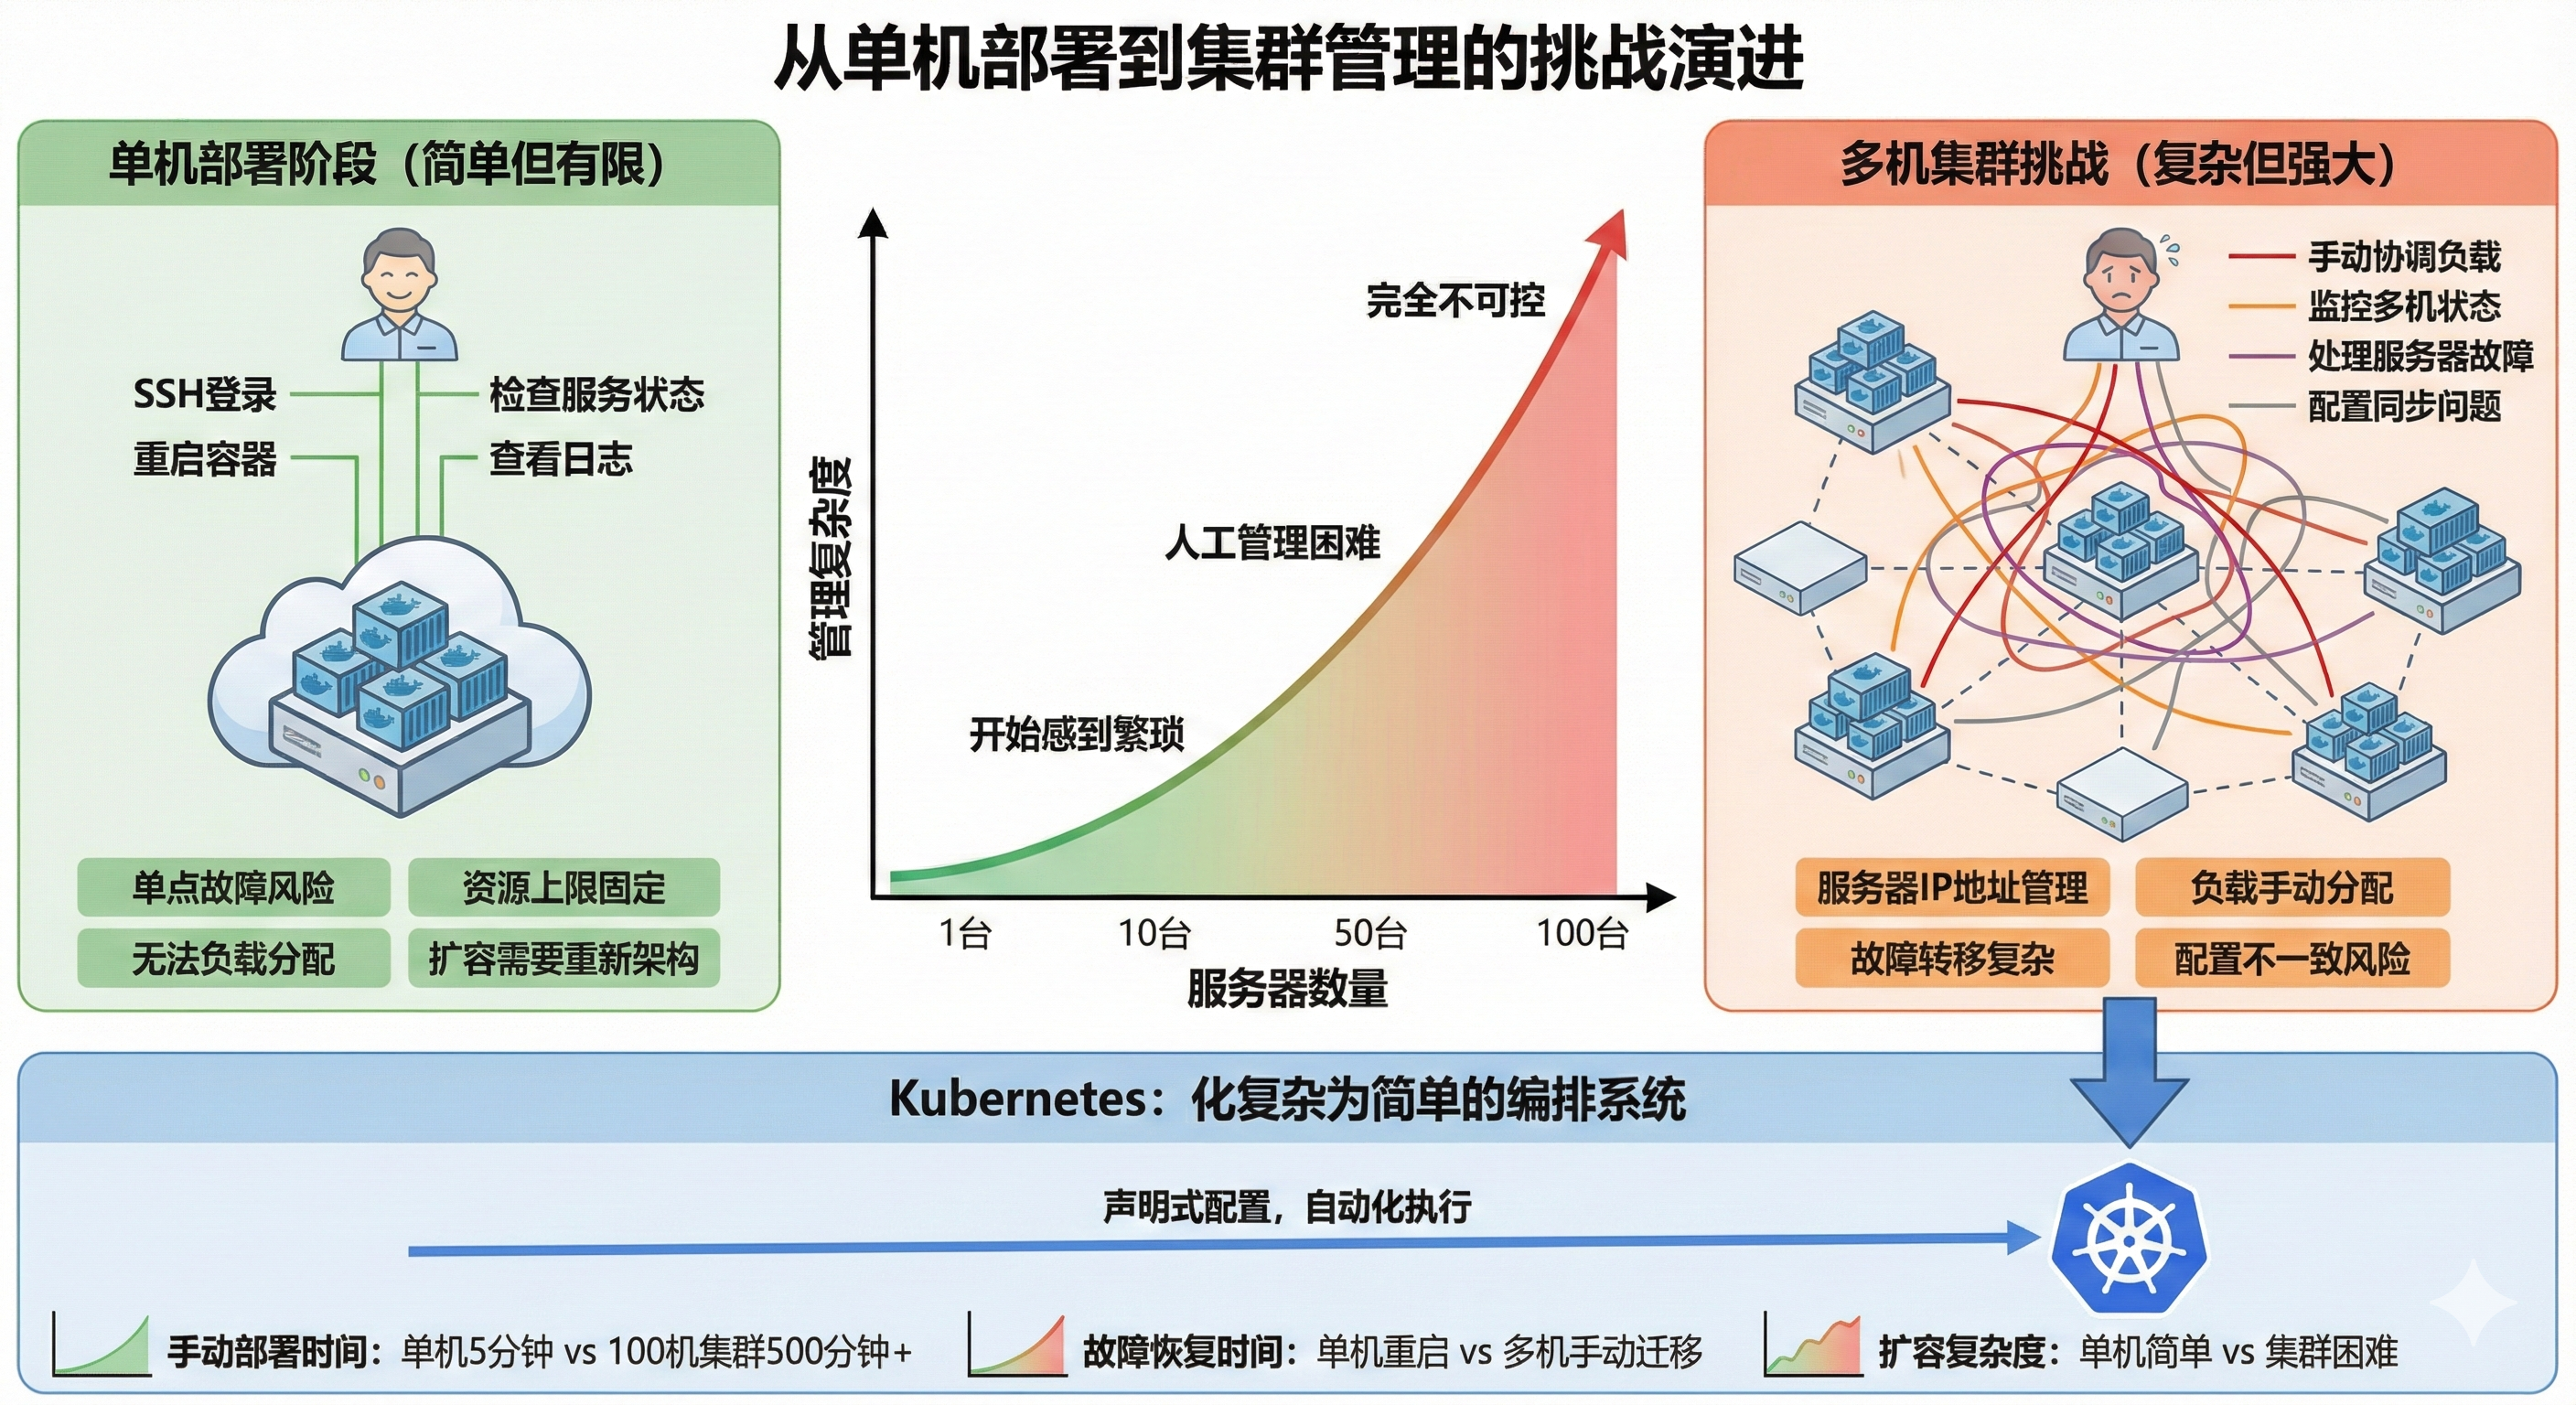
\includegraphics[width=0.9\textwidth]{figures/sec5/single-server-vs-cluster-management.png}
\caption{从单机部署到集群管理的挑战演进}
\label{fig:single-vs-cluster}
\end{figure}

如图\ref{fig:single-vs-cluster}所示，从单机部署向多机集群的扩展过程中，管理复杂度呈指数级增长，而Kubernetes正是为了解决这个根本性挑战而诞生的。

\subsubsection{Kubernetes：分布式系统的大脑}

Kubernetes（简称K8s）本质上是一个分布式的容器编排系统，但更准确地说，它是一个"分布式系统的操作系统"。如果把传统的操作系统比作管理单台计算机上各种程序运行的管家，那么Kubernetes就是管理整个数据中心中成千上万个容器协同工作的超级管家。

这个"超级管家"的核心价值在于将复杂的分布式系统管理抽象为简单的声明式操作。你不需要关心具体在哪台机器上运行什么容器，也不需要手动处理服务器故障和负载均衡，只需要告诉Kubernetes"我需要运行什么服务，需要多少个副本，需要什么样的资源"，它就会自动协调整个集群来实现你的期望。

Kubernetes的工作原理可以类比为一个拥有全局视野的智能调度中心。它持续监控整个集群中每台服务器的资源使用情况、每个容器的健康状态、每个服务的负载情况，然后基于这些信息做出智能的调度决策。当需要启动新容器时，它会选择最合适的服务器；当某台服务器过载时，它会自动将部分容器迁移到其他服务器；当某个容器崩溃时，它会立即在其他地方启动替代容器。

更重要的是，Kubernetes采用了"声明式"而非"命令式"的管理哲学。传统的运维方式是命令式的：你需要明确告诉系统执行每一个具体步骤，比如"在服务器A上启动容器X，在服务器B上启动容器Y，配置负载均衡器指向这两个容器"。而Kubernetes的声明式方式让你只需要描述期望的最终状态："我需要3个游戏服务器容器在运行，每个容器分配512MB内存"，然后K8s会自动分析当前状态与期望状态的差异，并执行必要的操作来达成目标。

\begin{figure}[htbp]
\centering
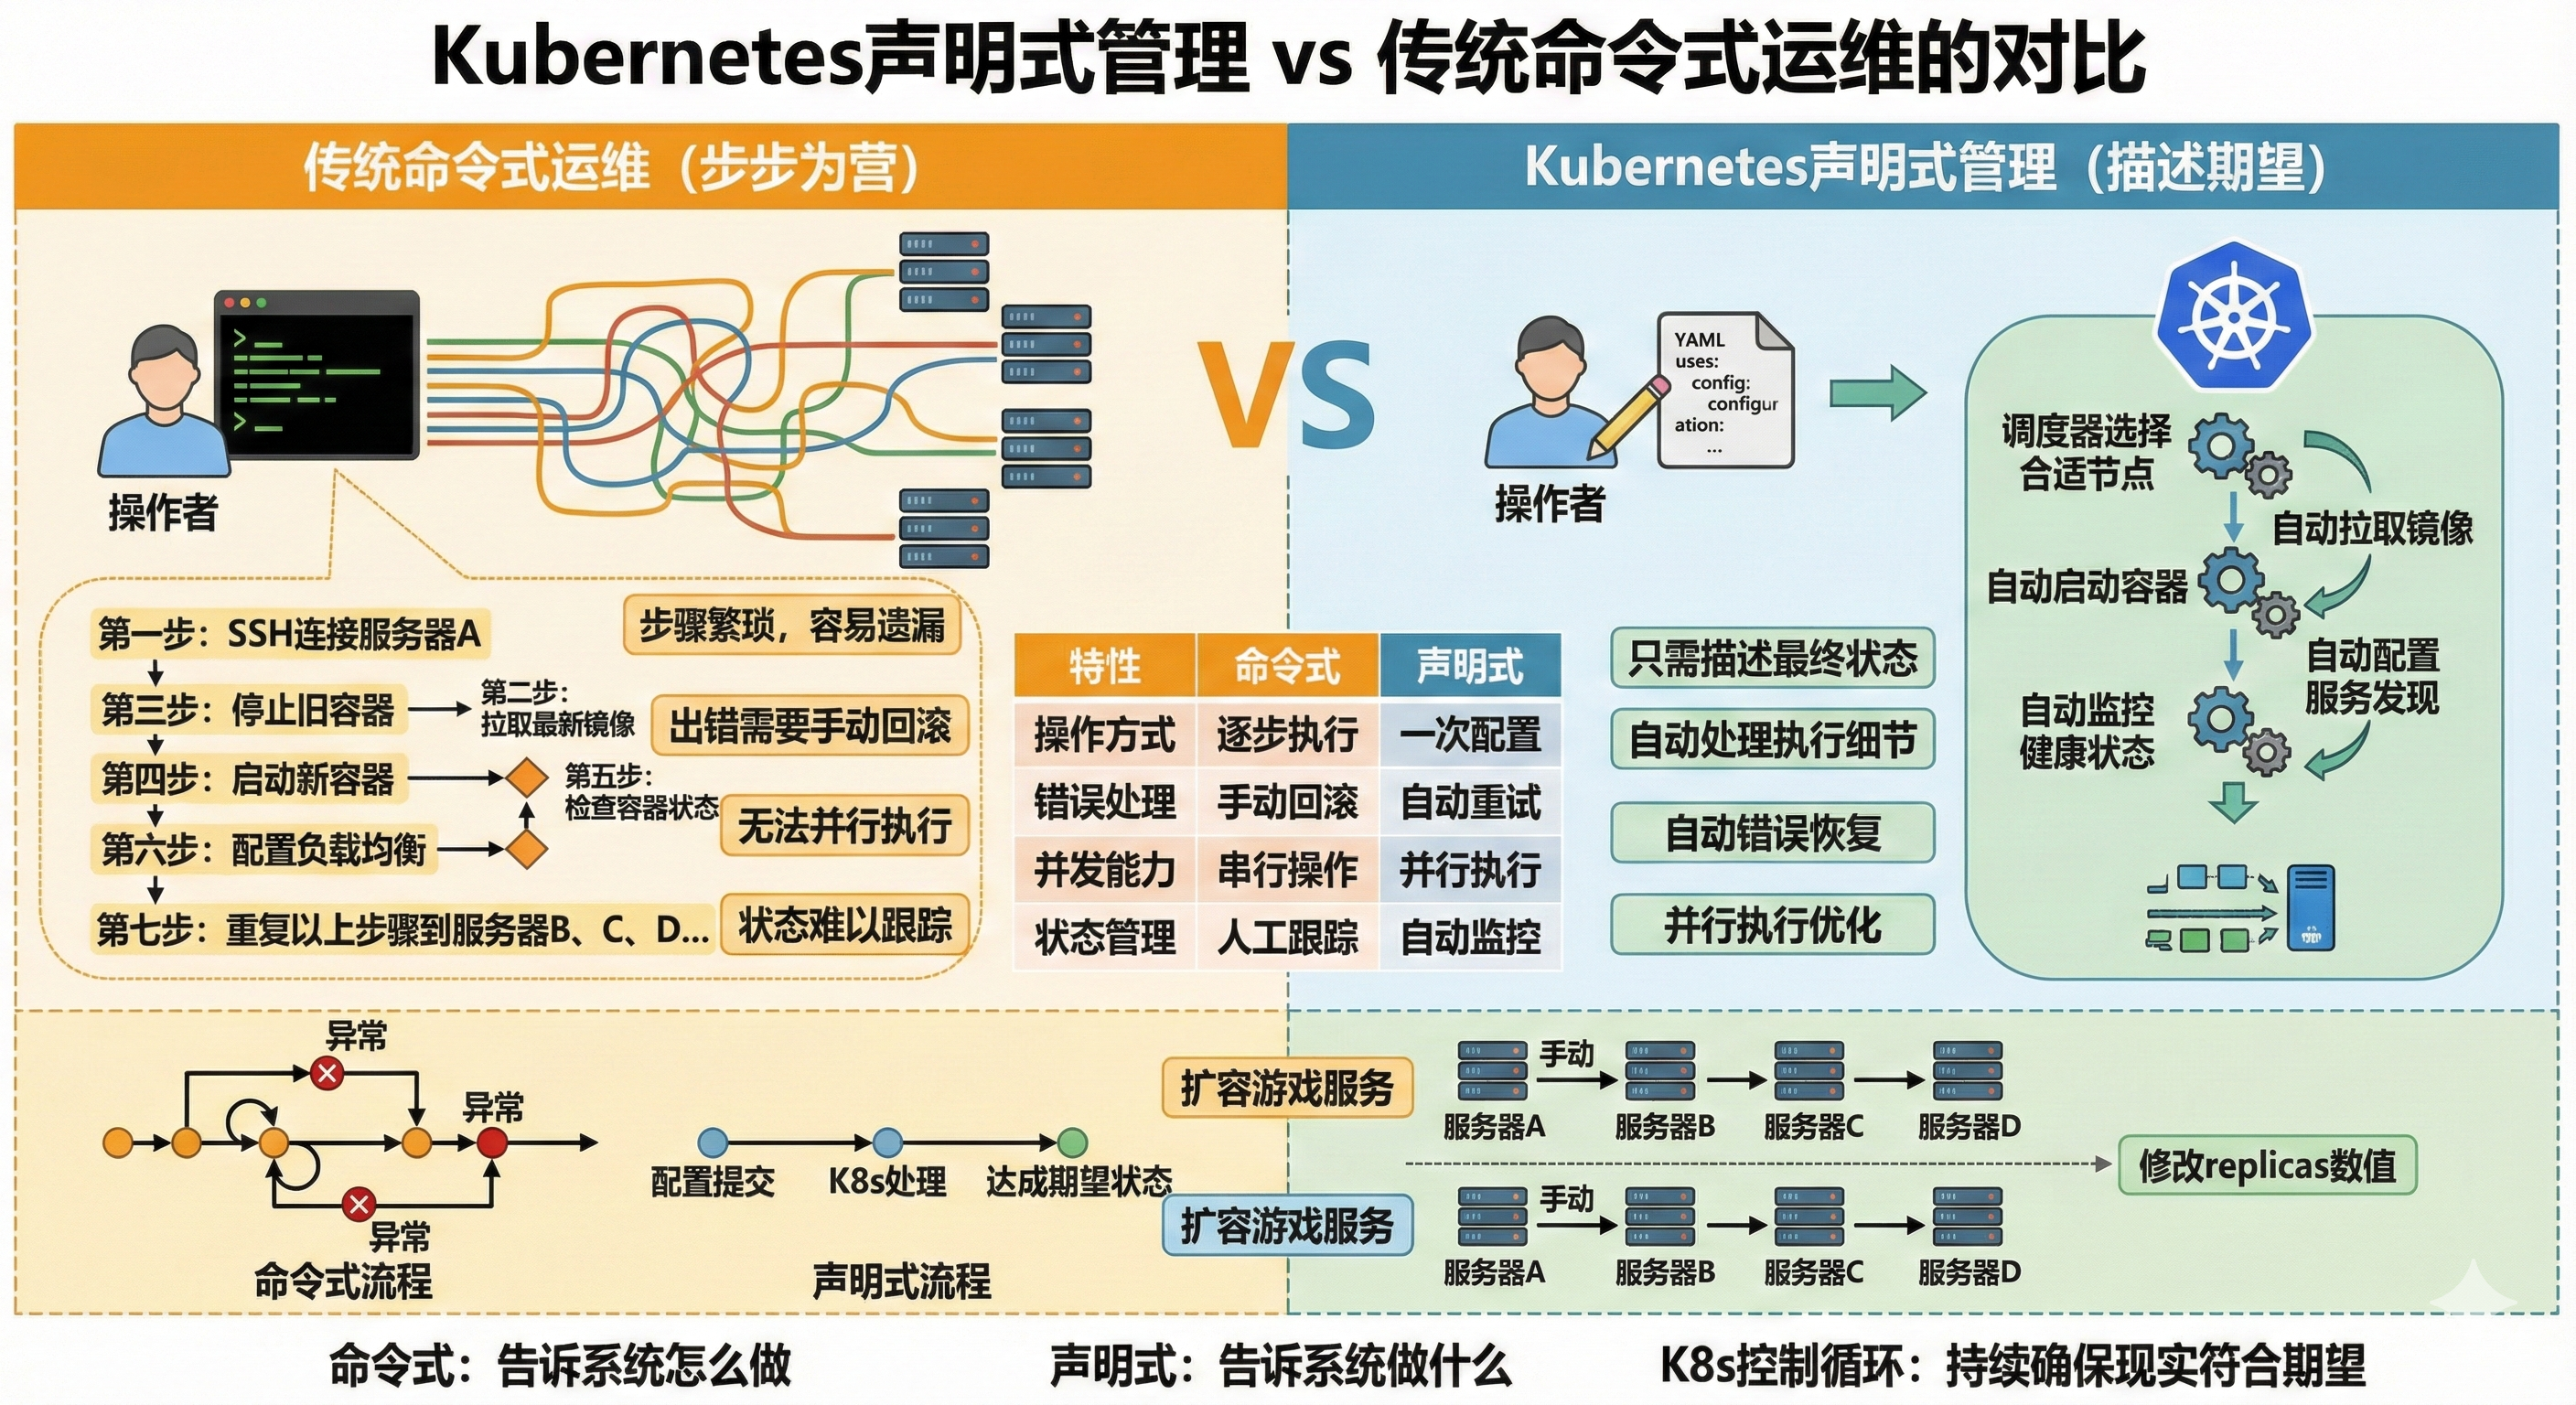
\includegraphics[width=0.9\textwidth]{figures/sec5/kubernetes-declarative-vs-imperative.png}
\caption{Kubernetes声明式管理 vs 传统命令式运维的对比}
\label{fig:declarative-vs-imperative}
\end{figure}

如图\ref{fig:declarative-vs-imperative}所示，这种声明式的设计哲学带来了巨大的运维效率提升。当你需要扩容时，只需要修改"期望副本数"这一个数字，K8s会自动处理后续的所有复杂操作；当你需要更新服务版本时，只需要修改镜像版本号，K8s会自动执行滚动更新，确保服务不中断；当某台服务器需要维护时，K8s会自动将其上的容器迁移到其他服务器，实现零停机维护。

下面是一个简单的 K8s 配置文件示例，定义了一个运行三个副本的游戏服务：
\begin{tcolorbox}[title=Kubernetes 部署示例]
\begin{lstlisting}[
    language=bash,
    basicstyle=\ttfamily\footnotesize,
    numbers=left,                   % 开启左侧行号
    numberstyle=\tiny\color{gray},  % 行号样式：灰色小号字体
    numbersep=5pt,                  % 行号与代码的距离
    aboveskip=0pt, belowskip=0pt,
    lineskip=-1pt,
    commentstyle=\color{gray},
    keywordstyle=\color{blue}\bfseries,
    breaklines=true,
    showstringspaces=false
]
apiVersion: apps/v1
kind: Deployment
metadata:
  name: game-server
spec:
  replicas: 3
  selector:
    matchLabels:
      app: game
  template:
    metadata:
      labels:
        app: game
    spec:
      containers:
      - name: game-server
        image: game/server:v1
        ports:
        - containerPort: 8080
        resources:
          requests:
            memory: "512Mi"
          limits:
            memory: "1Gi"
---
apiVersion: v1
kind: Service
metadata:
  name: game-service
spec:
  selector:
    app: game
  ports:
  - protocol: TCP
    port: 80
    targetPort: 8080
  type: LoadBalancer
\end{lstlisting}
\end{tcolorbox}
这份配置\texttt{Deployment} 定义了一个名为 \texttt{game-server} 的服务，期望运行 3 个副本（实例）。每个容器使用 \texttt{game/server:v1} 镜像，并将容器内的 8080 端口暴露出来。资源请求和限制设置了内存初始需求和上限，帮助调度器合理分配机器资源。\texttt{Service} 定义了一个负载均衡入口（类型为 \texttt{LoadBalancer}），通过服务名字将请求分发给标签为 \texttt{app=game} 的所有容器实例。

借助这份声明式配置，你只需一条命令 \texttt{kubectl apply -f deployment.yaml}，K8s 就会自动完成后端的调度、部署、负载均衡和健康检查，实现真正的自动化集群管理。这也正是 Kubernetes 作为分布式系统“大脑”的魅力所在，极大提高了复杂应用的扩展性、可靠性和运维效率。

回忆一下第四章的做法：我们手工维护Nginx的\texttt{upstream}列表来实现负载均衡，每次后端实例变化都要改写\texttt{nginx.conf}，逐条更新IP和端口，再执行\texttt{nginx -s reload}才能生效。到了Kubernetes，这个"把流量分发到一组可变后端"的问题并没有改变，只是由\textbf{Service}基于Pod的标签（Label）持续观察成员变化，并由\textbf{kube-proxy}组件自动刷新端点列表——你再也不需要手动维护一份服务器清单了。

实时战斗场景对延迟和抖动极为敏感，很多核心链路会选用UDP，以避免队头阻塞并缩短交互路径。从平台能力看，Kubernetes Service对UDP是原生支持的，端口声明后即可进行四层转发与负载分担。需要注意的是，常见的Nginx Ingress主要工作在HTTP/HTTPS语义层，默认并不能直接代理通用UDP流量，因此把游戏对战端口挂在标准Ingress之下，通常既不直观也不稳定。在生产环境中，更稳妥的做法是为游戏服单独创建\texttt{type: LoadBalancer}的Service，由云厂商或集群外部负载均衡器直接暴露UDP四层入口，避免不必要的协议转换。这里要明确区分L4与L7负载均衡：前者按传输层五元组转发，后者理解应用层协议与路由规则。游戏业务在网关设计时应先确定协议边界，再决定在哪一层实施流量治理。


\subsubsection{核心概念：K8s世界的组织架构}

要掌握Kubernetes，必须理解它的几个核心概念。这些概念构成了K8s管理容器化应用的基础框架，我们可以将其类比为一个现代化工厂的组织结构来理解。

\textbf{Cluster（集群）}是整个Kubernetes系统的边界，代表了所有被统一管理的计算资源的集合。就像一个工业园区包含了多个厂房、办公楼、仓库等设施一样，一个K8s集群包含了多台服务器、网络设备、存储系统等基础设施。集群提供了统一的资源池和管理界面，让运维人员可以将分散的硬件资源作为一个整体来使用。

\textbf{Node（节点）}是集群中的单台物理服务器或虚拟机，相当于工厂中的一个车间。每个Node都具备独立的计算、存储和网络能力，是承载实际工作负载的基础单元。Kubernetes的控制平面会持续监控每个Node的资源使用情况、健康状态，并根据这些信息做出智能的调度决策。当某个Node出现故障时，K8s会自动将其上的工作负载迁移到健康的Node上，确保服务不中断。

\textbf{Pod（容器组）}是Kubernetes中最小的部署和管理单元。一个Pod通常包含一个主要的应用容器和若干个辅助容器，它们共享网络和存储资源，必须被调度到同一个Node上一起运行。可以将Pod理解为车间里的一个工作小组，小组内的工人（容器）需要紧密协作，共享相同的工作环境。对于我们的游戏服务，一个Pod通常包含一个游戏服务器容器，以及可能的日志收集或监控辅助容器。

\textbf{Deployment（部署控制器）}负责管理Pod的生命周期，确保始终有期望数量的Pod实例在健康运行。它就像工厂里的生产主管，负责监督工作小组的数量和状态。如果某个Pod因为故障下线，Deployment会自动创建新的Pod替换；如果需要扩容，Deployment会启动更多Pod副本；如果需要更新服务版本，Deployment会协调滚动更新过程，确保服务连续性。

\textbf{Service（服务抽象）}为一组功能相同的Pod提供统一的访问入口和负载分发机制。它就像工厂的客服中心，外部客户无需知道具体哪个工作小组在处理自己的订单，只需要联系客服中心，Service会自动将请求分配给可用的Pod。Service还提供了服务发现功能，让不同的服务可以通过稳定的名称相互找到，而不用关心底层Pod的具体位置和IP地址。

第四章里我们实现过一个协调服务器：游戏服务器启动时向协调器注册自己的地址，客户端再向协调器查询可用的游戏服务器。在Kubernetes中，这套服务发现链路下沉为基础设施能力：\textbf{CoreDNS}会为每个Service自动生成域名（例如\texttt{game-server.default.svc.cluster.local}），集群内的任何Pod都可以通过域名直接访问其他服务，无需知道对方的IP地址。这标志着服务发现从应用层协议转向了平台层机制——对于登录、匹配等无状态服务，游戏服务器的代码中不再需要任何注册与发现的逻辑。不过，对于需要将玩家"粘"在特定战斗实例上的有状态场景，标准的Service负载均衡并不够用——这个问题我们将在后文的"思考"环节和第六章中进一步讨论。

\begin{figure}[htbp]
\centering
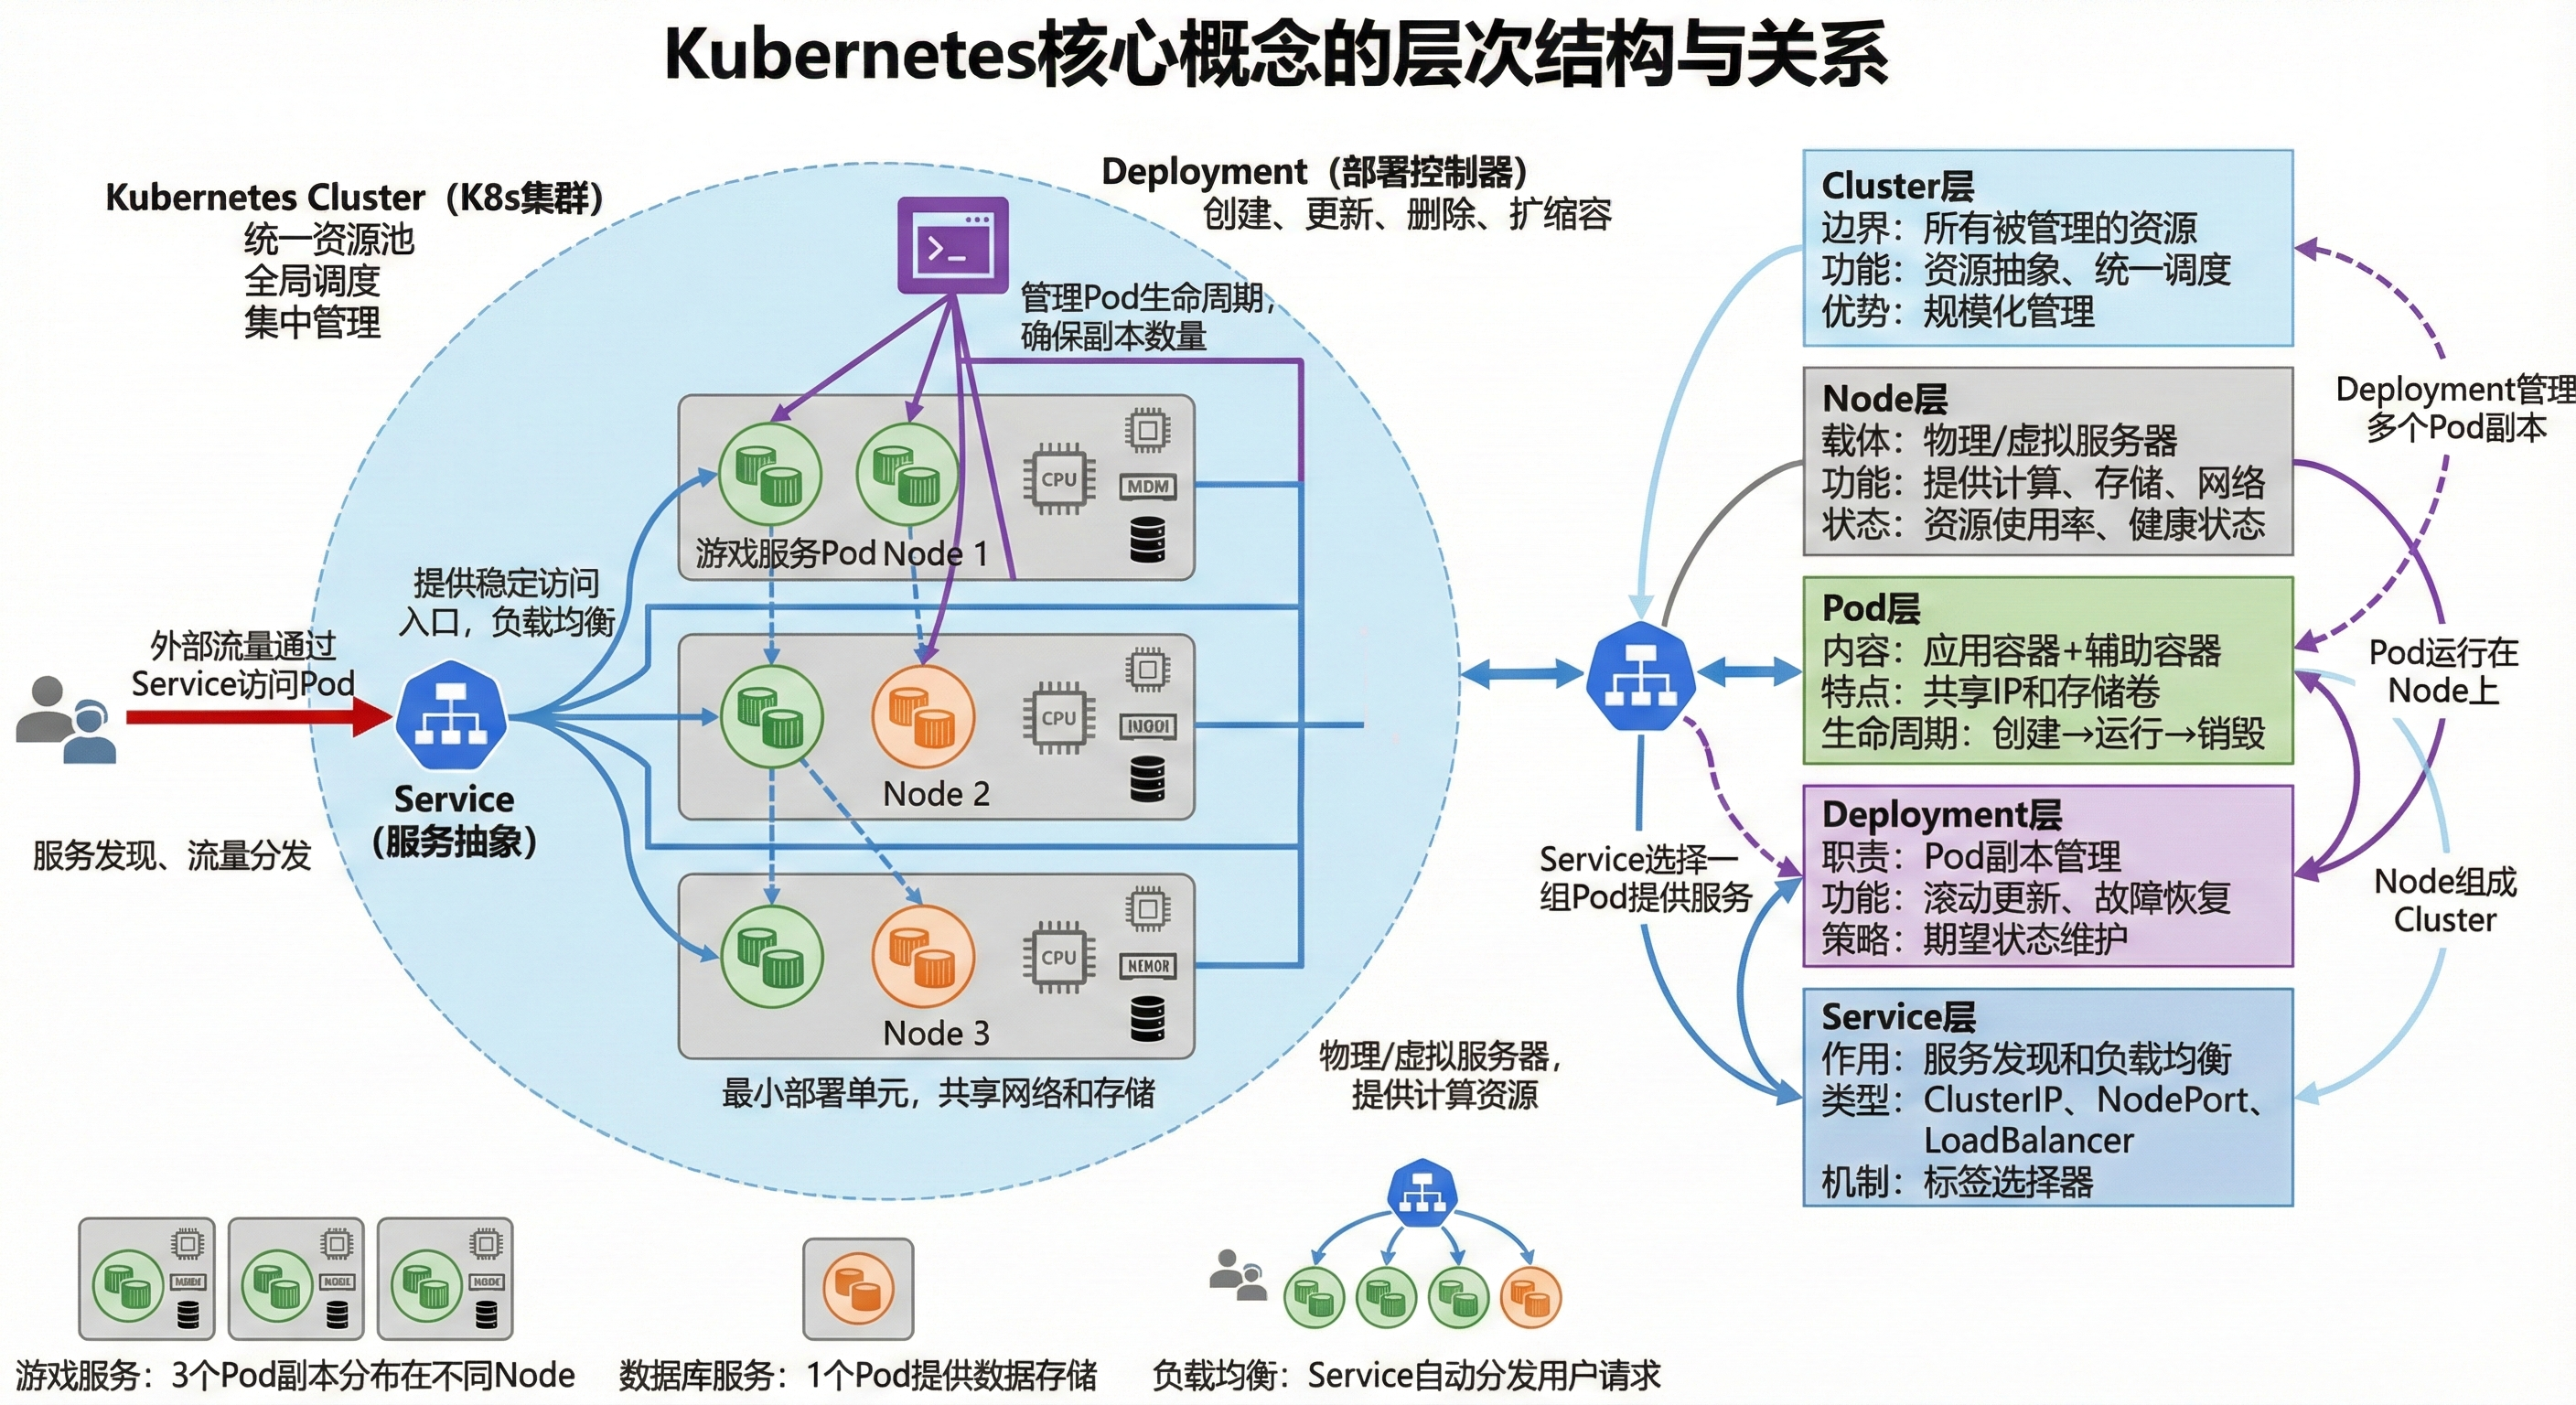
\includegraphics[width=0.9\textwidth]{figures/sec5/kubernetes-architecture-concepts.png}
\caption{Kubernetes核心概念的层次结构与关系}
\label{fig:k8s-concepts}
\end{figure}

如图\ref{fig:k8s-concepts}所示，这些概念形成了一个完整的层次化架构：Cluster提供资源边界，Node提供计算载体，Pod承载应用实例，Deployment管理Pod生命周期，Service提供访问入口，共同构成了Kubernetes强大的容器编排能力。

\subsubsection{工作流程：从配置到运行的自动化魔法}

了解了核心概念后，让我们深入了解Kubernetes是如何将我们的期望转化为实际运行的服务的。整个过程体现了现代云原生系统"配置驱动、自动执行"的设计理念。

当我们提交一份Deployment配置时，实际上是在向Kubernetes描述一个期望状态：我们希望有多少个Pod在运行，每个Pod使用什么镜像，需要多少资源等等。Kubernetes的控制循环（Control Loop）会持续比较当前实际状态与期望状态，并自动执行必要的操作来消除差异。

声明式管理的关键不在"一次下发命令"，而在持续运行的\textbf{Reconciliation Loop}。控制器不断执行"观察现状、对比期望、采取动作、再次观察"的闭环，使系统逐步逼近期望状态。这种机制属于Level-triggered思路，关注的是"现在是否达标"，而不是"刚刚发生了什么"。与之对照，Edge-triggered更依赖事件边沿，一旦事件处理链路中断，就可能留下状态空洞。在云原生控制面里，即便某次消息丢失，下一轮循环仍会重新发现偏差并自动修正。因而系统鲁棒性来自反复校准，而非假设每条通知都可靠送达且只执行一次。用游戏场景来讲，运营者只需声明"城门始终保持3名守卫"，某个守卫倒下后，控制逻辑会在后续轮次自动补位，而不是等待人工逐条下达替补指令。

这个过程的第一步是调度（Scheduling）。Kubernetes的调度器会分析每个新Pod的资源需求，然后在整个集群中寻找最合适的Node。调度算法会考虑多种因素：Node的剩余资源是否足够、是否有特殊的亲和性要求、是否需要避免某些Node等。调度决策完成后，kubelet（运行在每个Node上的代理程序）会接收指令并在本地启动相应的容器。

实际上，K8s的调度过程远比"找一台空闲机器"复杂。调度器采用两阶段流程：先做过滤（Filter），根据资源请求、亲和与反亲和、污点容忍等约束，把明显不合适的Node剔除；再做打分（Score），对候选Node按多种指标评分并排序，选择当前最合适者。从理论上看，这本质上是一个多维资源装箱问题——CPU、内存、带宽与拓扑同时参与决策，在计算复杂性上通常被视为NP-hard，因此工程实现强调近似最优与可扩展性。其思想脉络可追溯到Google的Borg，随后发展到Omega，再到今天的Kubernetes。若借用游戏比喻，调度器像在给玩家分配房间：不只看空位多少，还要兼顾延迟、容量与地域，只有把这些维度同时纳入权衡，系统才可能在高负载下维持稳定体验与资源利用率。

第二步是服务注册与发现。当Pod成功启动后，它会自动注册到相应的Service中。Service通过标签选择器（Label Selector）机制找到属于它的Pod，并将这些Pod的IP地址加入到负载均衡池中。这个过程是完全自动的，新启动的Pod会立即开始接收外部请求，下线的Pod会立即从负载均衡池中移除。


还记得第四章中我们为游戏服务器实现的健康检查端点吗？协调服务器定期向每台游戏服务器发送HTTP请求，如果连续几次没有响应，就将其从可用列表中移除。Kubernetes采用同样的思路，但拆分成了更清晰的两类探针：\textbf{Liveness Probe}在进程"活着但已失效"时触发重启，\textbf{Readiness Probe}在实例尚未就绪时将其临时移出Service的负载均衡池。核心思想不变，只是由平台统一执行，而非业务代码重复实现。
第三步是持续监控与自愈。Kubernetes会持续监控每个Pod的健康状态，通过健康检查（Health Check）机制检测Pod是否正常工作。如果发现Pod异常，Deployment控制器会立即启动新的Pod来替换故障实例。这种自愈能力让系统具备了很强的容错性，单个Pod的故障不会影响整体服务的可用性。

\begin{figure}[htbp]
\centering
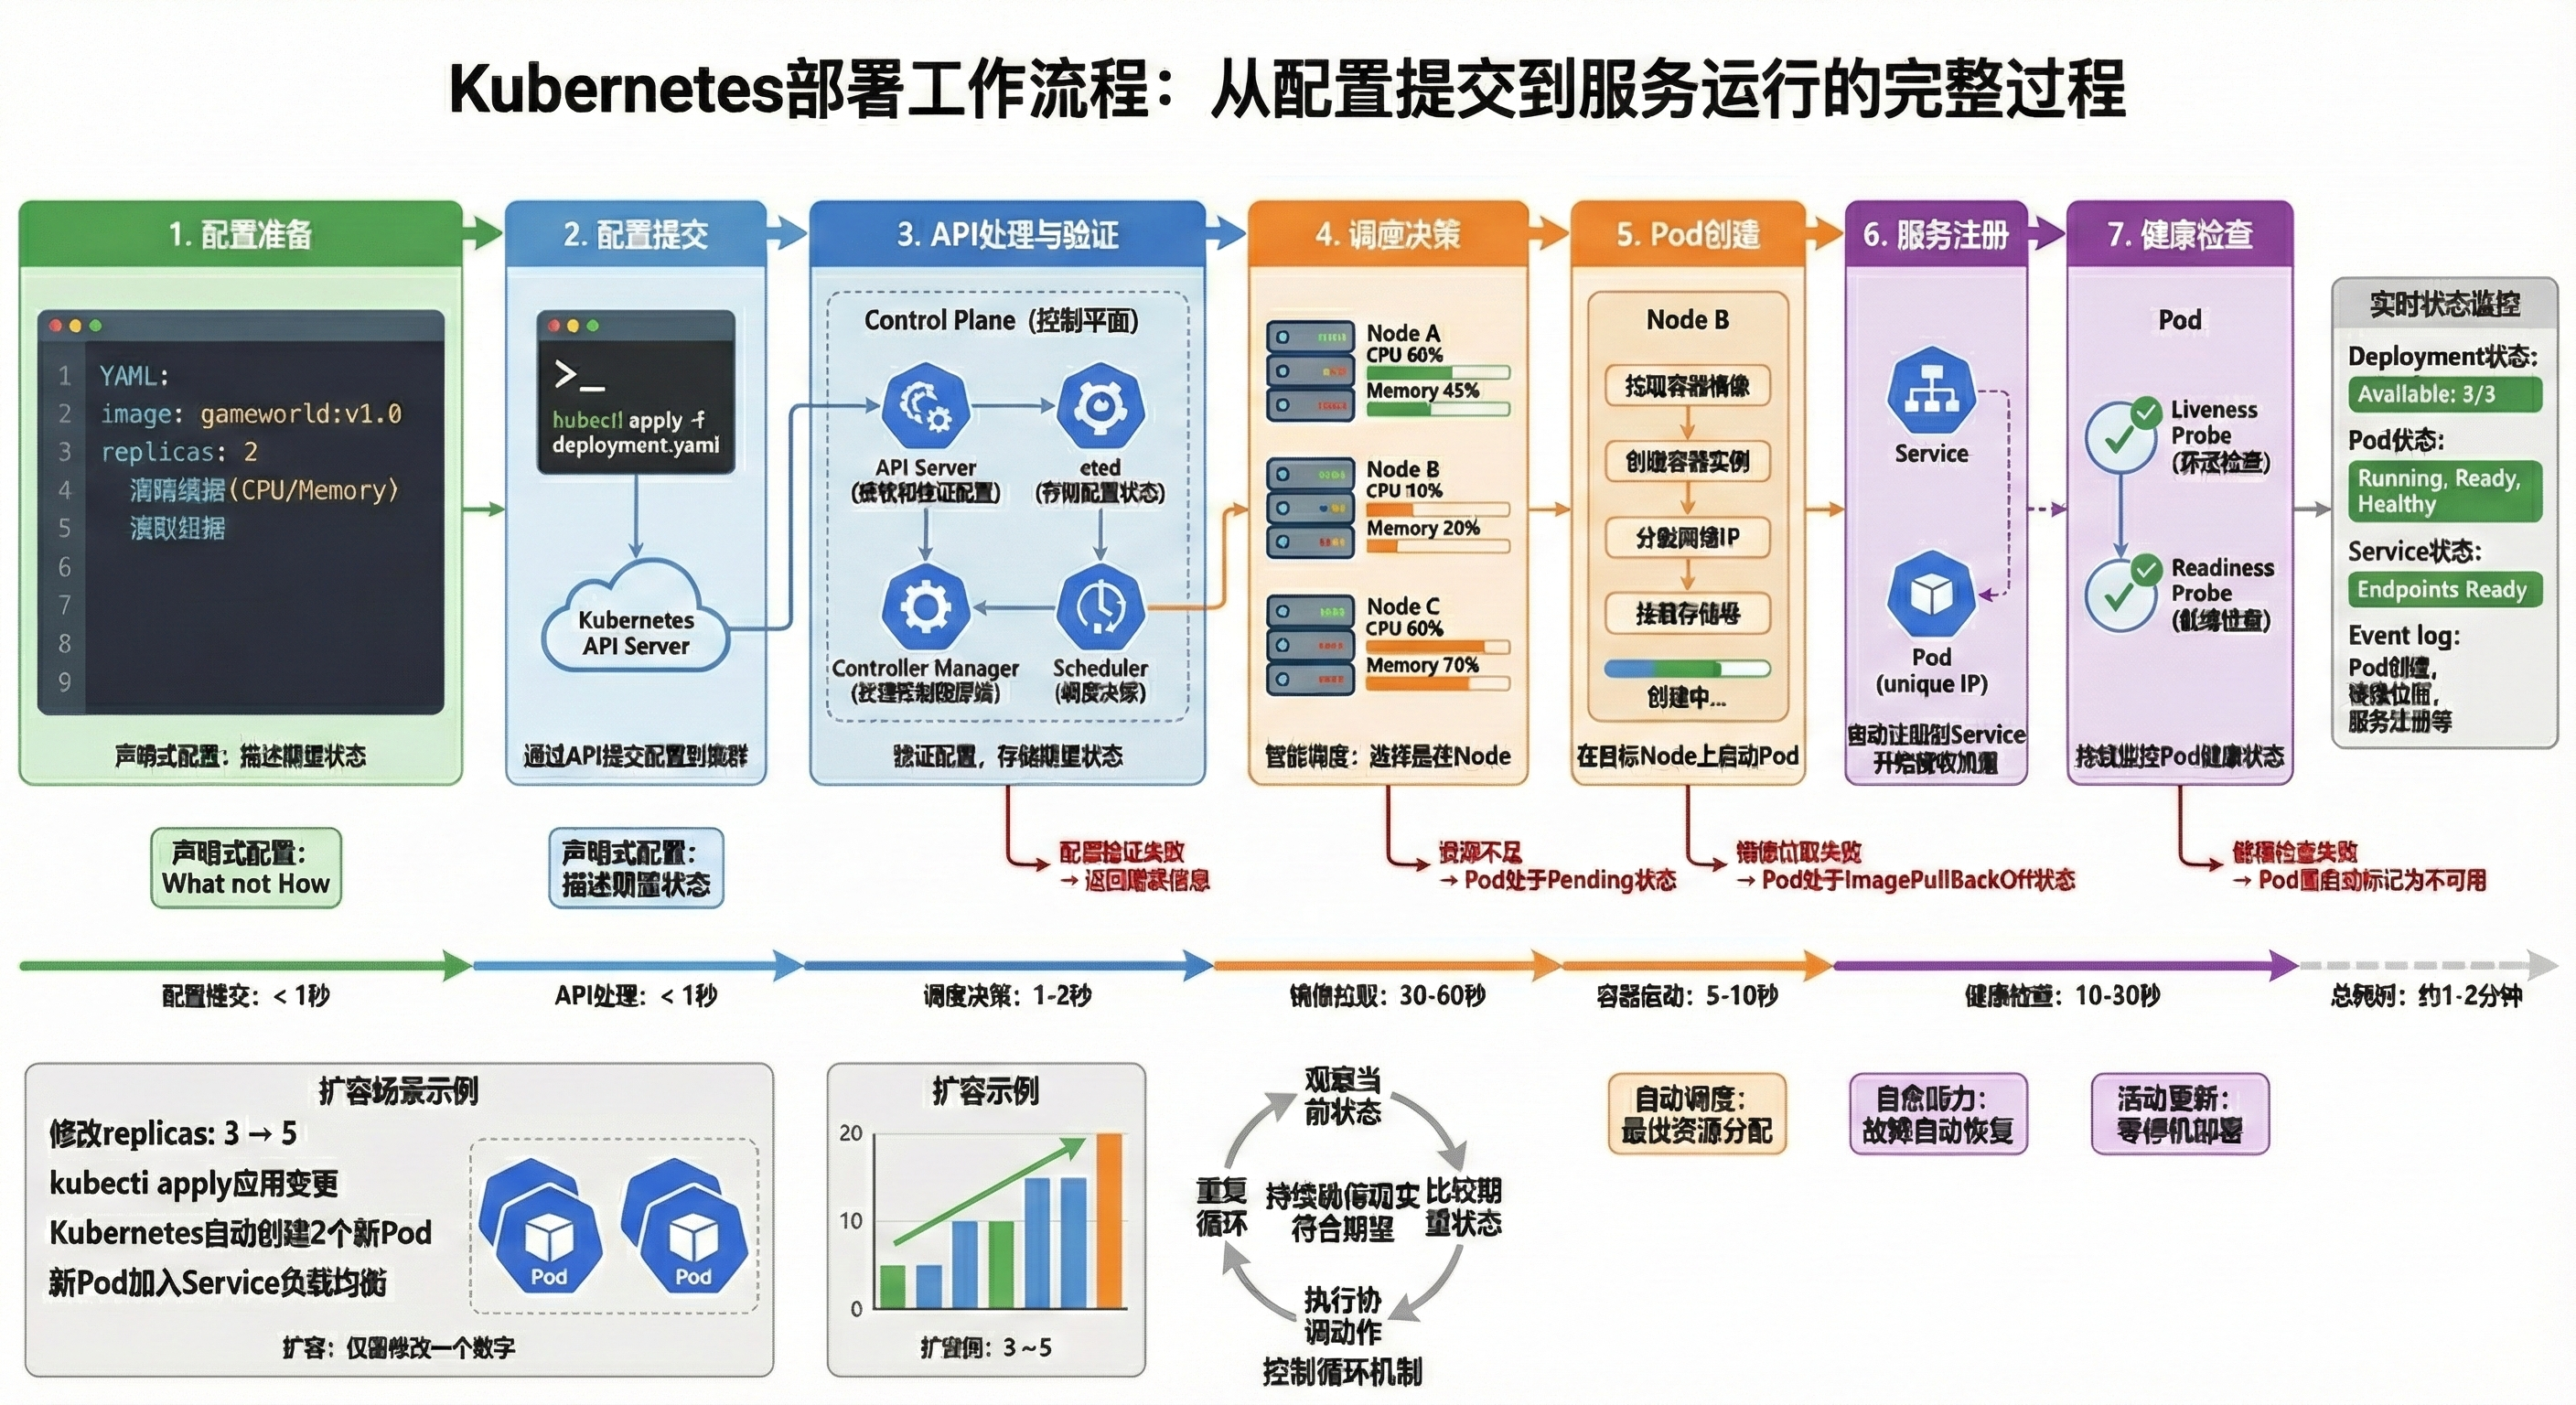
\includegraphics[width=0.9\textwidth]{figures/sec5/kubernetes-deployment-workflow.png}
\caption{Kubernetes部署工作流程：从配置提交到服务运行的完整过程}
\label{fig:k8s-workflow}
\end{figure}

如图\ref{fig:k8s-workflow}所示，最令人印象深刻的是扩容过程的简化。当我们需要应对流量增长时，只需要修改Deployment配置中的副本数（replicas），K8s就会自动启动新的Pod实例。调度器会选择合适的Node，kubelet会拉取镜像并启动容器，Service会自动将新Pod加入负载均衡，整个过程无需人工干预，通常在几分钟内就能完成。

理解了上述核心概念之后，读者可以参照附录C.3的实战指南，亲手完成从编写YAML配置、执行\texttt{kubectl apply}到监控部署状态的完整流程，体验"声明期望，自动实现"的云原生部署理念。


在Kubernetes的设计假设里，Deployment面向的是无状态工作负载，任何一个Pod都应当可以被随时替换。这套假设对大多数Web服务非常合适，但游戏服务端往往在内存中维护玩家会话——例如第三章连接池模型里保存的连接上下文、匹配状态与短期战斗数据，都会绑定到当前进程。因此工程上常见两条路：其一是把会话状态外置到Redis，让业务Pod尽量回到可替换的无状态形态；其二是采用StatefulSet，为Pod提供稳定网络标识与持久命名，再配合\textbf{Session Affinity}固定流量。前者更符合云原生弹性与故障恢复思路，但每次读写状态都可能引入额外网络时延与一致性成本；后者更接近传统游戏分区服架构，迁移门槛较低，却会牺牲一部分调度自由度与横向伸缩效率。这两类方案的容量评估、故障演练与选型方法将在第六章做进一步展开。


%\subsection{“弹性” 的奥义：迎接百万玩家的云端扩容术}
%\paragraph{本节目标} 理解弹性扩容，掌握 K8s 自动扩缩容逻辑。
%\paragraph{写作建议}
%\begin{enumerate}
%    \item 以 “固定服务器浪费 / 卡顿” 痛点，引出弹性（按负载调资源）。
%    \item 讲扩容逻辑：按 CPU 阈值（超 80\% 加 Pod，低于 30\% 减 Pod），Service 自动分请求。
%    \item 提 Node 扩容：Pod 不够时，云厂商自动加服务器。
%\end{enumerate}

\subsection{“弹性”的奥义：迎接百万玩家的云端扩容术}

在第四章中，当玩家负载增加时，我们的应对方式是：手动开通新的云服务器，部署游戏服务，向协调服务器注册，再修改Nginx配置——整个过程全靠人工。而当负载下降需要缩容时，更加麻烦：必须先把目标服务器上的玩家迁移到其他服务器（还记得第四章的"迁移玩家"机制吗？），确认没有活跃会话后才能安全关闭。这是一种应用层的伸缩方式——扩缩容的每一步都需要业务逻辑的配合。而在K8s的世界里，思路完全不同：你只需要声明"我希望CPU使用率保持在70\%以下"，平台就会自动增减Pod实例，Service自动调整流量分发。扩缩容从"人工操作服务器"变成了"声明期望状态"，这是一次根本性的思维转换。

\subsubsection{资源困境：当固定配置遇上波动流量}

在传统的服务器部署模式中，我们通常会基于业务高峰期的流量需求来配置服务器规格和数量。这种"按最坏情况准备"的策略虽然能够保证高峰期的服务质量，但却带来了严重的资源浪费问题。想象一下你经营着一家火爆的在线游戏：周五晚上8点，同时在线人数可能达到5万人，此时需要50台服务器才能保证流畅体验；而周二上午10点，在线人数可能只有5000人，理论上5台服务器就足够了。

这种资源配置困境的本质是"静态思维"与"动态现实"之间的根本矛盾。传统的IT架构假设负载是相对稳定和可预测的，因此采用了固定配置的设计思路。但互联网时代的业务负载具有强烈的波动性和不可预测性，这种静态配置必然导致要么资源过剩造成浪费，要么资源不足影响用户体验。

更深层的问题在于，互联网流量的波动模式远比我们想象的复杂。除了可以预见的周期性波动——工作日vs周末、白天vs夜晚、节假日效应等，还存在大量突发性和病毒式的流量爆炸。一个游戏主播的突然推荐、一次版本更新的Bug修复、一个网络热梗的病毒式传播，都可能在几分钟内让服务器负载暴增数十倍。

如果始终维持50台服务器运行，那么大部分时间里有90\%的计算资源在空转，每月产生巨额的无效成本。相反，如果为了节省成本而按照平均流量配置服务器，那么在流量高峰期就会出现严重的性能瓶颈。玩家会遭遇连接超时、操作卡顿甚至无法进入游戏等糟糕体验。这种"要么浪费钱，要么丢用户"的两难困境，是所有面向C端用户的互联网服务都必须面对的现实挑战。

\begin{figure}[htbp]
\centering
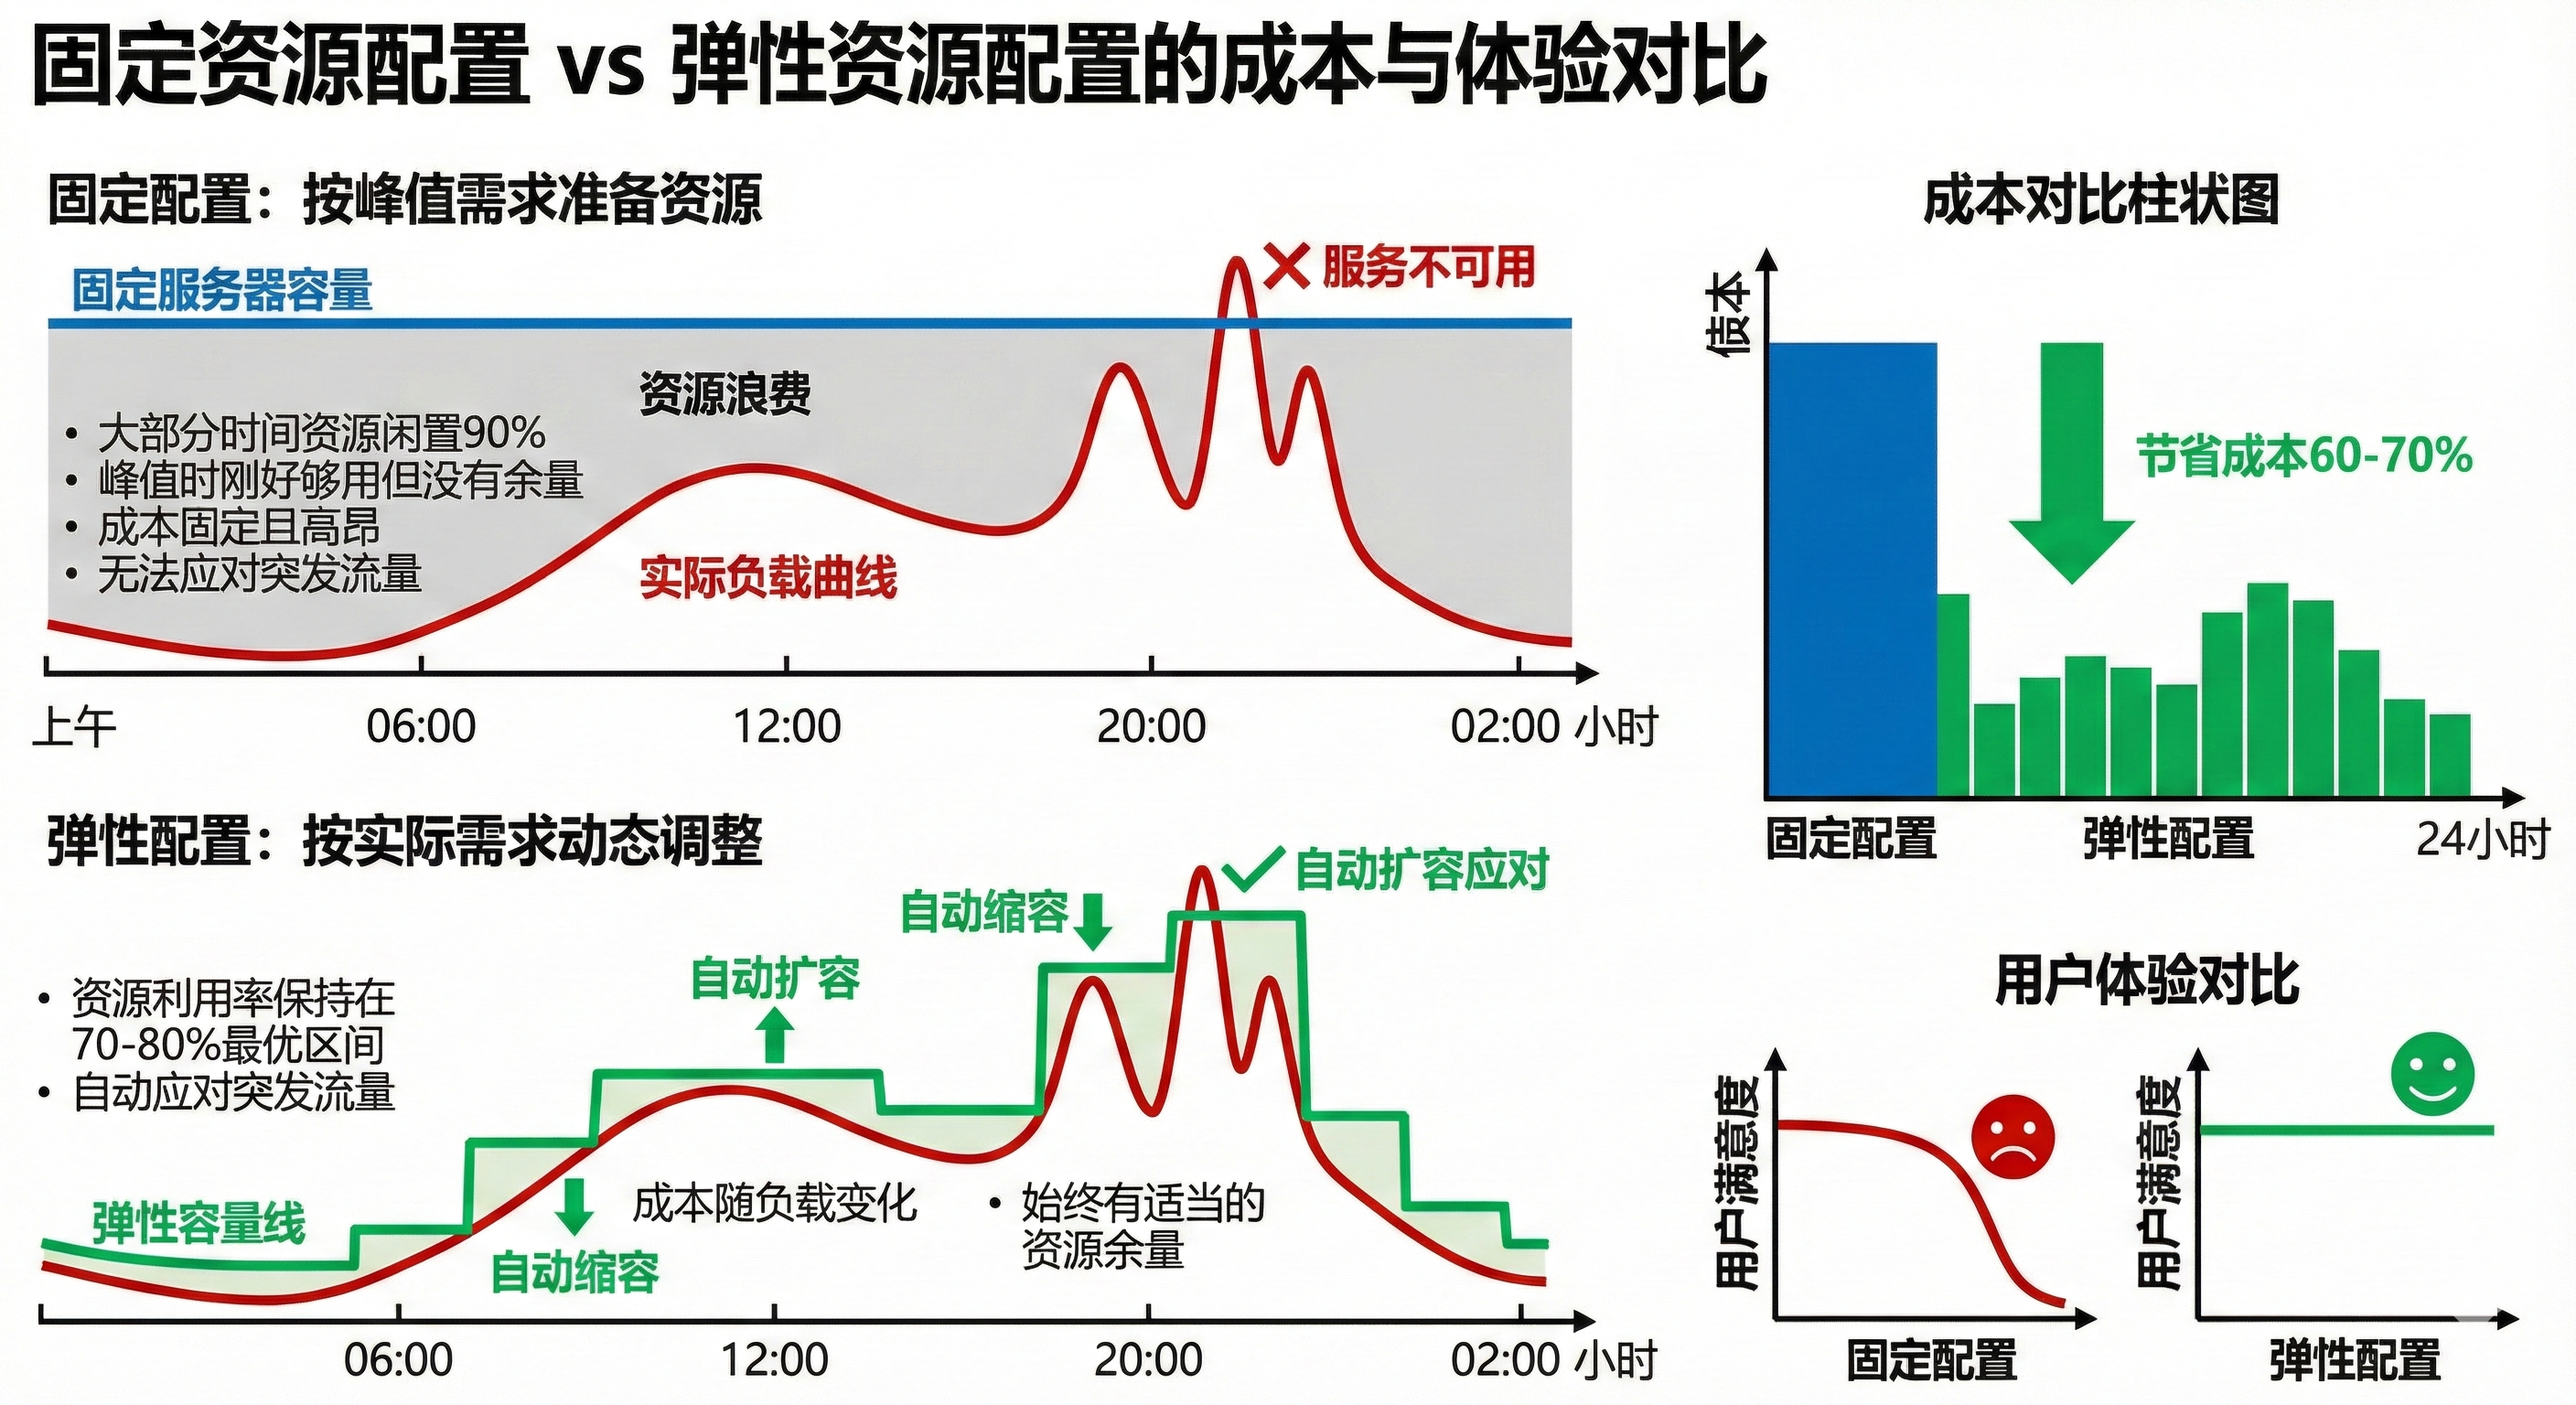
\includegraphics[width=0.9\textwidth]{figures/sec5/fixed-vs-elastic-resources.png}
\caption{固定资源配置 vs 弹性资源配置的成本与体验对比}
\label{fig:fixed-vs-elastic}
\end{figure}

如图\ref{fig:fixed-vs-elastic}所示，传统的固定配置模式在处理波动性负载时存在结构性缺陷，而弹性配置能够实现成本与性能的动态平衡。

\subsubsection{弹性扩容的核心思想：让资源像水一样流动}

"弹性扩容"的核心价值就是要彻底解决资源配置与流量波动之间的矛盾。它代表了一种全新的资源管理哲学：不再将服务器数量视为固定的静态配置，而是将其转变为根据实时负载动态调整的弹性变量。这种转变的意义远不止技术层面的优化，更是思维模式从"拥有资源"向"使用资源"的根本转变。

弹性扩容的工作原理可以类比为现代城市的交通管理系统。在交通高峰期，系统会自动调配更多的公交车上路、开放更多的车道、延长信号灯时间；在交通低峰期，则会减少运营车辆、关闭部分车道、缩短信号灯周期。这种动态调节不仅提升了整体效率，也避免了资源的无效占用。

在云计算环境中，弹性扩容通过持续监控关键指标（如CPU使用率、内存占用率、网络IO、响应时间等）来感知系统负载状态。当这些指标超过预设阈值时，系统会自动触发扩容操作：启动更多的服务实例、分配更多的计算资源、增加更多的服务器节点。当负载回落时，则执行相反的缩容操作，将多余的资源释放回资源池中供其他应用使用。

这种"按需分配，用完即还"的资源管理模式带来了多重价值。从成本角度看，它将固定的资本支出转化为变动的运营支出，让成本曲线与收入曲线更加匹配；从性能角度看，它确保系统始终运行在合理的负载区间内，避免了过载导致的性能下降；从运维角度看，它将复杂的容量规划决策转化为简单的策略配置，大大降低了人工干预的需要。

更重要的是，弹性扩容体现了云原生架构的一个核心理念：将基础设施视为可编程的资源。通过将扩缩容逻辑编码为策略配置，我们实际上是在"编程"整个数据中心的行为模式，让庞大的基础设施能够像软件程序一样精确、快速、自动地响应业务需求变化。

\subsubsection{HPA：Pod级别的智能呼吸}

Horizontal Pod Autoscaler（HPA，水平Pod自动扩缩器）是Kubernetes提供的Pod级别弹性扩容解决方案。HPA的设计哲学体现了控制论中的反馈控制原理：通过持续监测系统状态，将其与期望状态进行比较，然后执行相应的调节动作来消除偏差。

HPA的工作机制可以类比为人体的呼吸系统。当人体进行剧烈运动时，肌肉对氧气的需求急剧增加，血液中的氧气浓度下降、二氧化碳浓度上升。大脑的呼吸中枢感知到这种变化后，会自动加快呼吸频率、增大呼吸深度，以满足增加的氧气需求。当运动结束后，呼吸又会自然回归到平静状态。这种自动调节是无意识的、持续的、精确的。

类似地，HPA通过metrics server持续收集Pod的资源使用指标，当发现CPU使用率超过设定阈值（比如70\%）时，就会向Deployment控制器发出扩容指令，增加Pod副本数量。当新的Pod启动并开始分担负载后，平均CPU使用率下降，系统重新回到平衡状态。如果负载持续较低，HPA则会触发缩容操作，减少Pod数量以节省资源。

\begin{figure}[htbp]
\centering
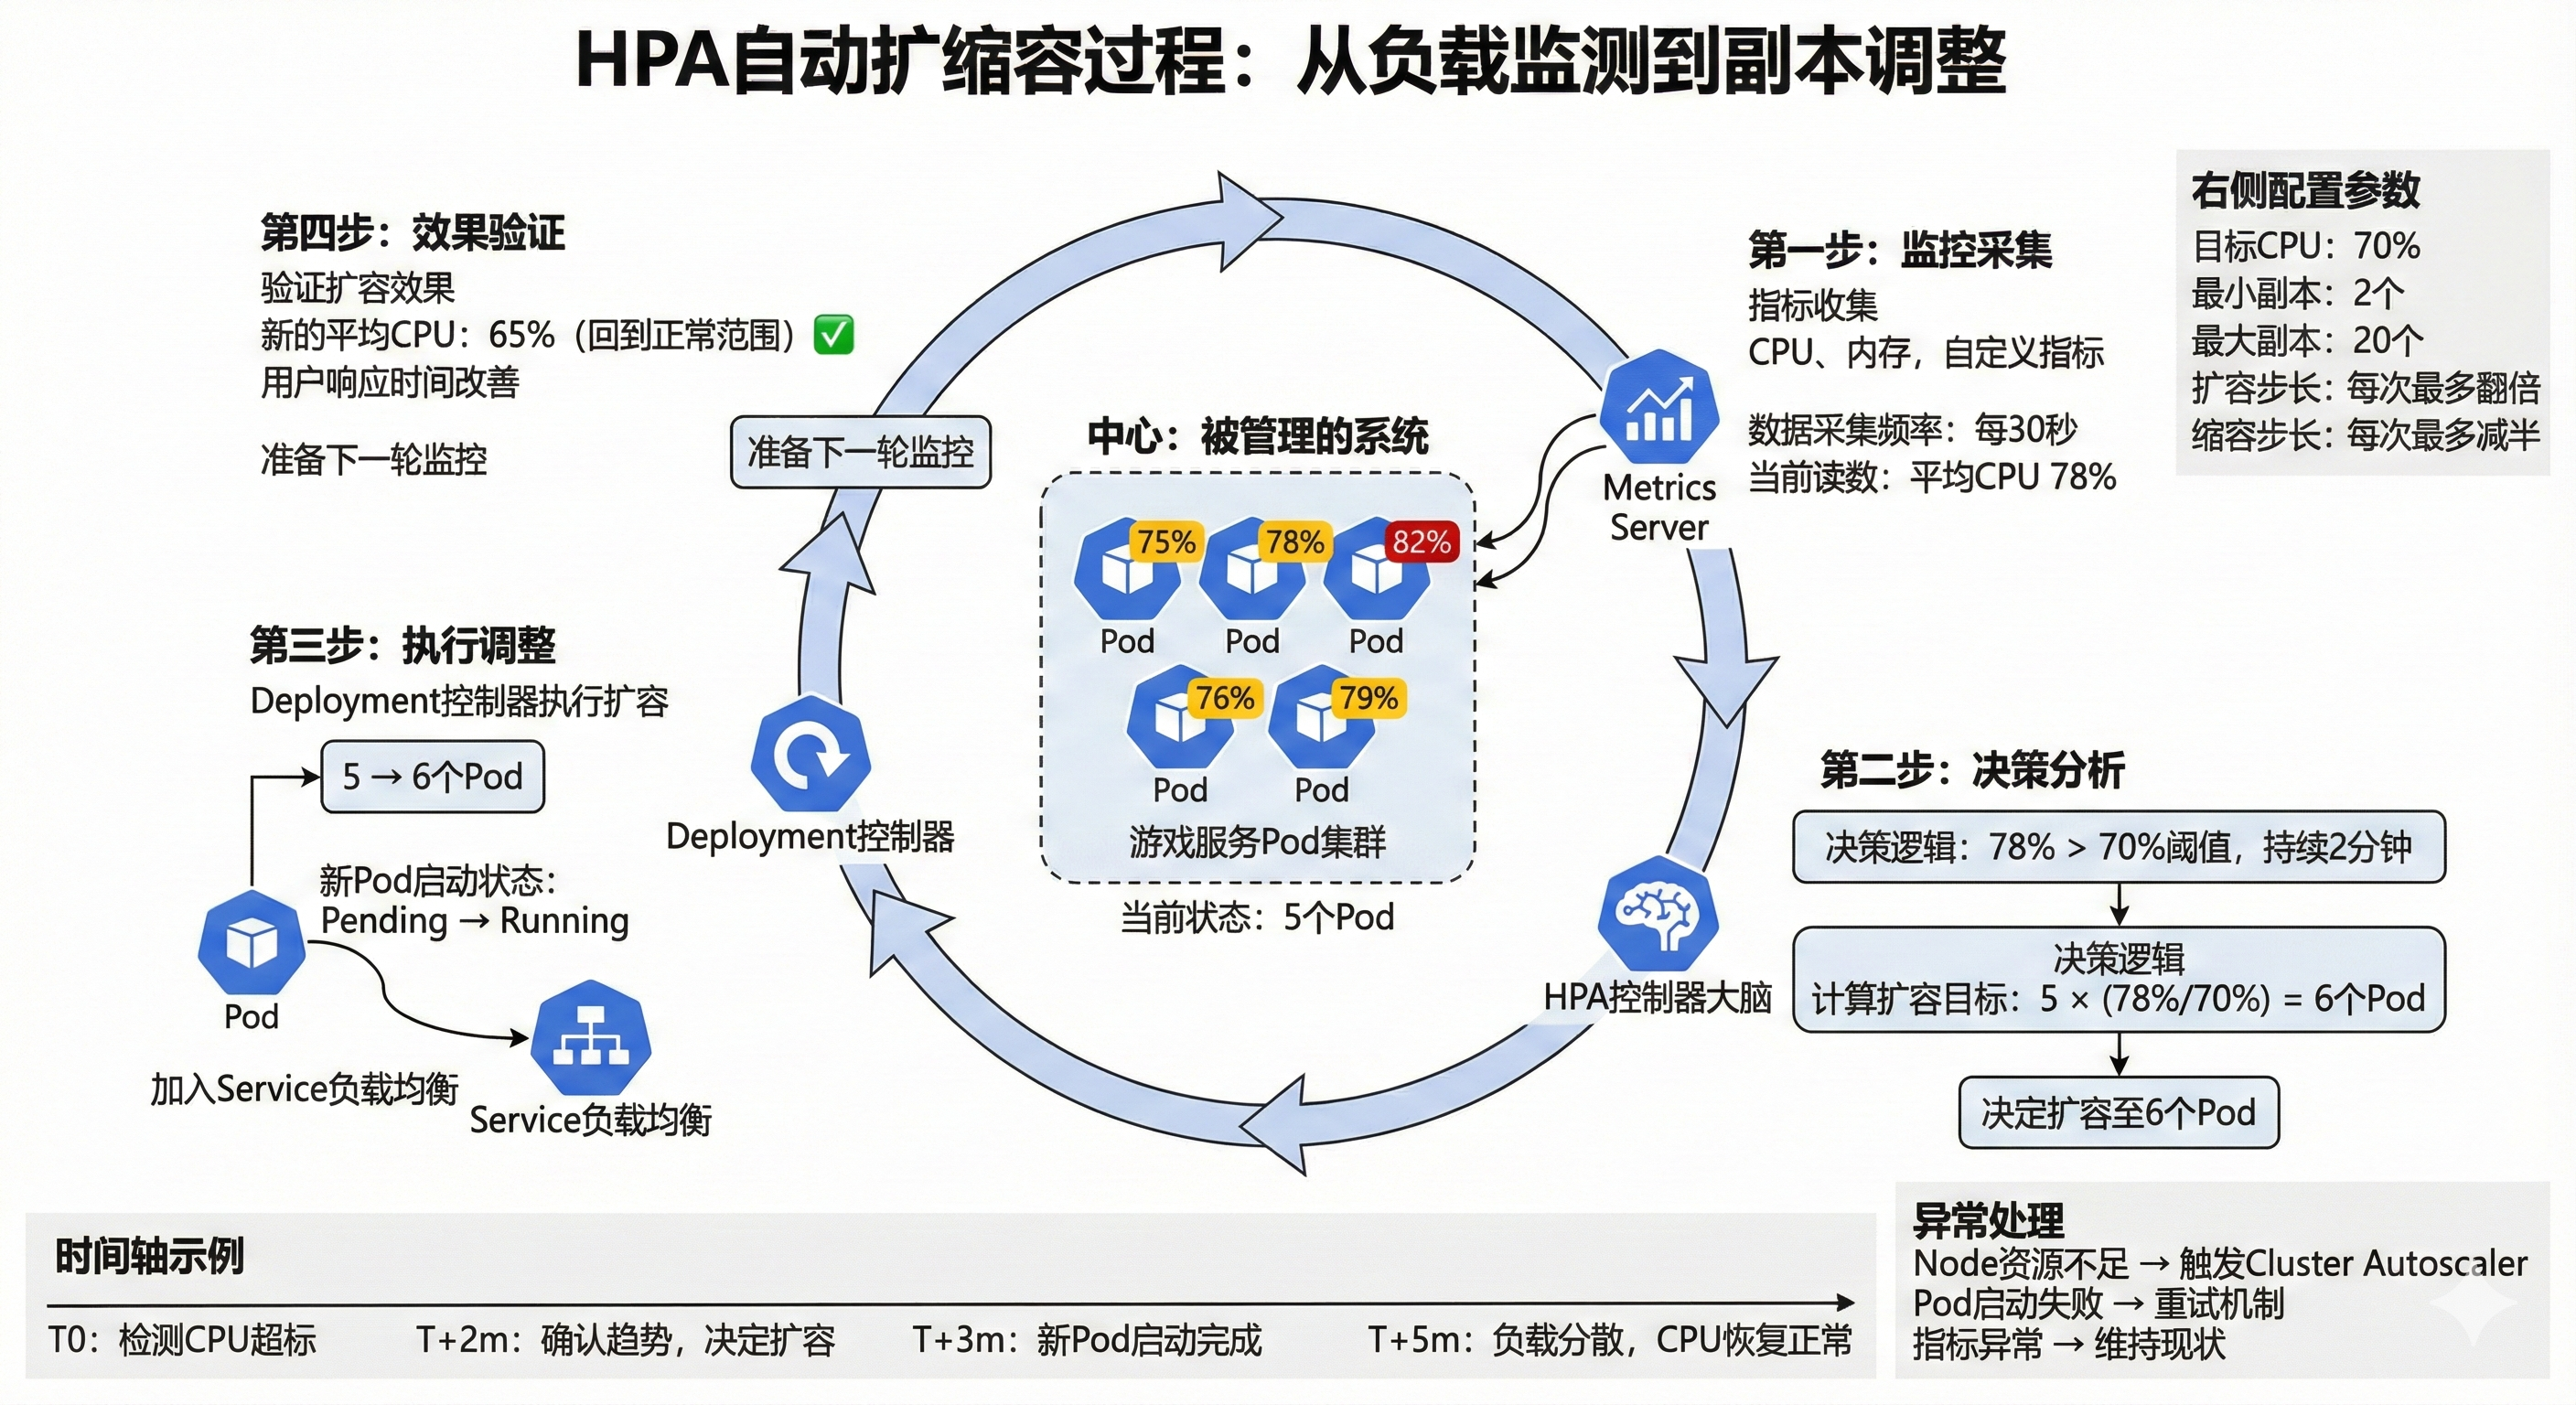
\includegraphics[width=0.9\textwidth]{figures/sec5/hpa-scaling-process.png}
\caption{HPA自动扩缩容过程：从负载监测到副本调整}
\label{fig:hpa-scaling}
\end{figure}

HPA的智能性体现在其多层次的决策机制上。首先是多指标综合评估：不仅仅关注CPU使用率，还会综合考虑内存使用率、网络IO、自定义业务指标等多个维度，避免单一指标可能导致的误判。其次是防抖动机制：通过设置观察窗口期和变化幅度限制，避免因短期波动导致的频繁扩缩容。最后是渐进式调整：每次扩缩容都采用相对温和的步长，给系统足够的时间来响应变化。

在实际的游戏场景中，HPA通常会配置为多阶梯的响应策略。当CPU使用率在60-80\%之间时，属于正常运行区间，不触发任何操作；当超过80\%时，开始扩容，每次增加当前副本数的50\%；当低于30\%且持续一定时间后，开始缩容，每次减少当前副本数的25\%。这种非线性的响应策略既保证了扩容的及时性，又确保了缩容的稳健性。

HPA的配置相对简单，但需要仔细考虑几个关键参数：目标CPU使用率通常设置在70\%左右，既保证了充足的处理能力，又留有应对突发负载的余量；最小副本数确保基本的服务可用性和容错能力；最大副本数防止扩容失控导致成本爆炸；扩缩容的冷却期避免系统震荡。

HPA的真正价值在于它将复杂的容量管理决策自动化了。运维人员不再需要半夜起床处理流量突增，不再需要猜测明天需要多少服务器，不再需要在成本和性能之间做艰难的权衡。只需要设定合理的策略参数，HPA就会7×24小时不间断地监控和调节，确保系统始终运行在最佳状态。

从控制理论的视角看，HPA本质上可以看作一个比例控制器（P-controller），它根据当前观测指标与目标指标的偏差，按比例直接调整副本数。Kubernetes常用的计算关系可写为：
\[
\texttt{desiredReplicas}=\lceil \texttt{currentReplicas}\times \texttt{currentMetric}/\texttt{targetMetric}\rceil
\]
例如目标CPU使用率为70\%，当前达到140\%，且现有3个副本时，系统会计算$\lceil 3\times 140/70\rceil=6$，因此扩容到6个副本。这种机制只有P项，没有I项和D项，实现简单但容易出现稳态误差与来回振荡；为降低抖动，HPA默认设置约10\%的容忍区间，小幅偏差不触发动作。然而它仍受限于约15秒的采样周期叠加Pod启动时间，端到端最短响应通常也在45秒量级，而且本质上仍是被动响应负载变化，无法提前预测流量尖峰。此外需要注意，HPA的决策基于所有Pod的平均指标值，如果只有个别实例因热点玩家集中而过载，而其余实例负载很低，平均值可能仍在阈值以内，导致扩容不被触发——这种"热点稀释"现象在游戏场景中尤为常见。更先进的PID控制器和预测式扩缩容将在第六章讨论。

实际生产中，HPA的缩容不能简单地把Pod立即终止，尤其是承载活跃游戏会话的服务——否则玩家会在对局中被强制断开，造成体验和业务损失。

\texttt{terminationGracePeriodSeconds}的作用，就是在收到终止信号后为Pod预留一个优雅退出窗口，让其有机会将玩家状态持久化并引导客户端重连。需要注意的是，这个宽限期是硬超时——如果一局游戏持续20分钟而宽限期只有默认的30秒，Pod仍会被强制终止。因此对于长时间运行的游戏会话，更务实的做法是在PreStop阶段触发"停止接收新对局"的排水状态，让当前对局自然结束，而非指望宽限期能覆盖整局时长。同时可结合\texttt{PreStop} Hook在容器退出前执行清理逻辑，例如通知在线玩家、持久化房间状态、以及从流量入口中摘除并完成连接排空。此外，\texttt{PodDisruptionBudget}（PDB）可约束中断期间的最小可用副本数，防止缩容、升级或节点维护叠加时把服务压到不可用边缘。用游戏场景类比，就是比赛进行时不能直接拆球场，必须等当前比赛结束，或先把球员安全转移到其他可用场地后再处理原场地。

\subsubsection{集群自动扩容：当容器装不下时自动加机器}

当Pod级别的扩容达到Node资源的物理上限时，就需要启动Node级别的扩容，即向集群中添加更多的云服务器。这个过程涉及与云厂商API的深度集成，需要Kubernetes能够自主决定何时购买新服务器、选择什么规格、以及如何将新服务器纳入集群管理。

Cluster Autoscaler（集群自动扩缩器）是实现Node级弹性的核心组件，它的工作原理可以类比为一个智能的办公楼管理系统。当所有现有的办公室都被占满，还有新员工需要入驻时，管理系统会自动租用新的楼层；当某些楼层长期空置时，会将剩余员工集中到其他楼层，然后退租空置楼层以节省成本。

Cluster Autoscaler的触发机制有两个主要场景。扩容触发：当调度器发现有Pod因为资源不足而无法调度到任何现有Node上时，这些Pod会处于Pending状态。Cluster Autoscaler监控到这种情况后，会分析这些Pending Pod的资源需求，然后请求云厂商创建合适规格的新虚拟机实例。新Node启动并加入集群后，调度器就可以将Pending的Pod调度到新Node上运行。

缩容触发相对复杂一些：Cluster Autoscaler会持续监控每个Node的资源利用率，当发现某个Node的利用率长期低于阈值（通常是50\%）时，会评估是否可以将该Node上的所有Pod迁移到其他Node。如果迁移操作不会导致资源不足或违反Pod的调度约束，就会执行Node缩容：首先将该Node标记为不可调度，然后逐个迁移Pod到其他Node，最后将空Node从集群中移除并释放云服务器资源。

Node级扩容的一个关键优势是智能的实例类型选择。现代云厂商通常提供数十种不同规格的虚拟机实例：计算优化型（高CPU核心数）、内存优化型（大内存容量）、存储优化型（高IOPS磁盘）、网络优化型（高带宽）、通用均衡型等。Cluster Autoscaler可以根据Pending Pod的资源需求特征，自动选择最合适且最经济的实例类型。

例如，对于CPU密集型的游戏逻辑计算，Cluster Autoscaler会选择计算优化型实例；对于需要大量缓存数据的Redis服务，会选择内存优化型实例；对于处理大量玩家连接的网关服务，会选择网络优化型实例。这种智能匹配不仅提升了资源利用效率，也避免了"用牛刀杀鸡"式的资源浪费。

\subsubsection{多层弹性：构建真正的自适应系统}

Pod级扩容与Node级扩容的结合，构成了一个完整的多层弹性体系。这种设计体现了现代分布式系统的层次化架构思想：每一层都专注于解决特定范围内的问题，层与层之间通过标准化接口协作，共同实现系统整体的智能行为。

在这个多层体系中，HPA负责应用层的精细化调度。它关注的是Pod级别的资源使用效率，通过增减Pod副本数量来匹配实时负载。HPA的响应速度很快（通常在1-2分钟内），因为它只需要在现有Node上启动或停止容器，不涉及基础设施的变化。

Cluster Autoscaler负责基础设施层的宏观扩展。它关注的是集群整体的资源容量，通过增减Node数量来突破现有集群的资源边界。Cluster Autoscaler的响应速度相对较慢（通常需要3-5分钟），因为它需要与云厂商API交互来创建或销毁虚拟机实例。

\begin{figure}[htbp]
\centering
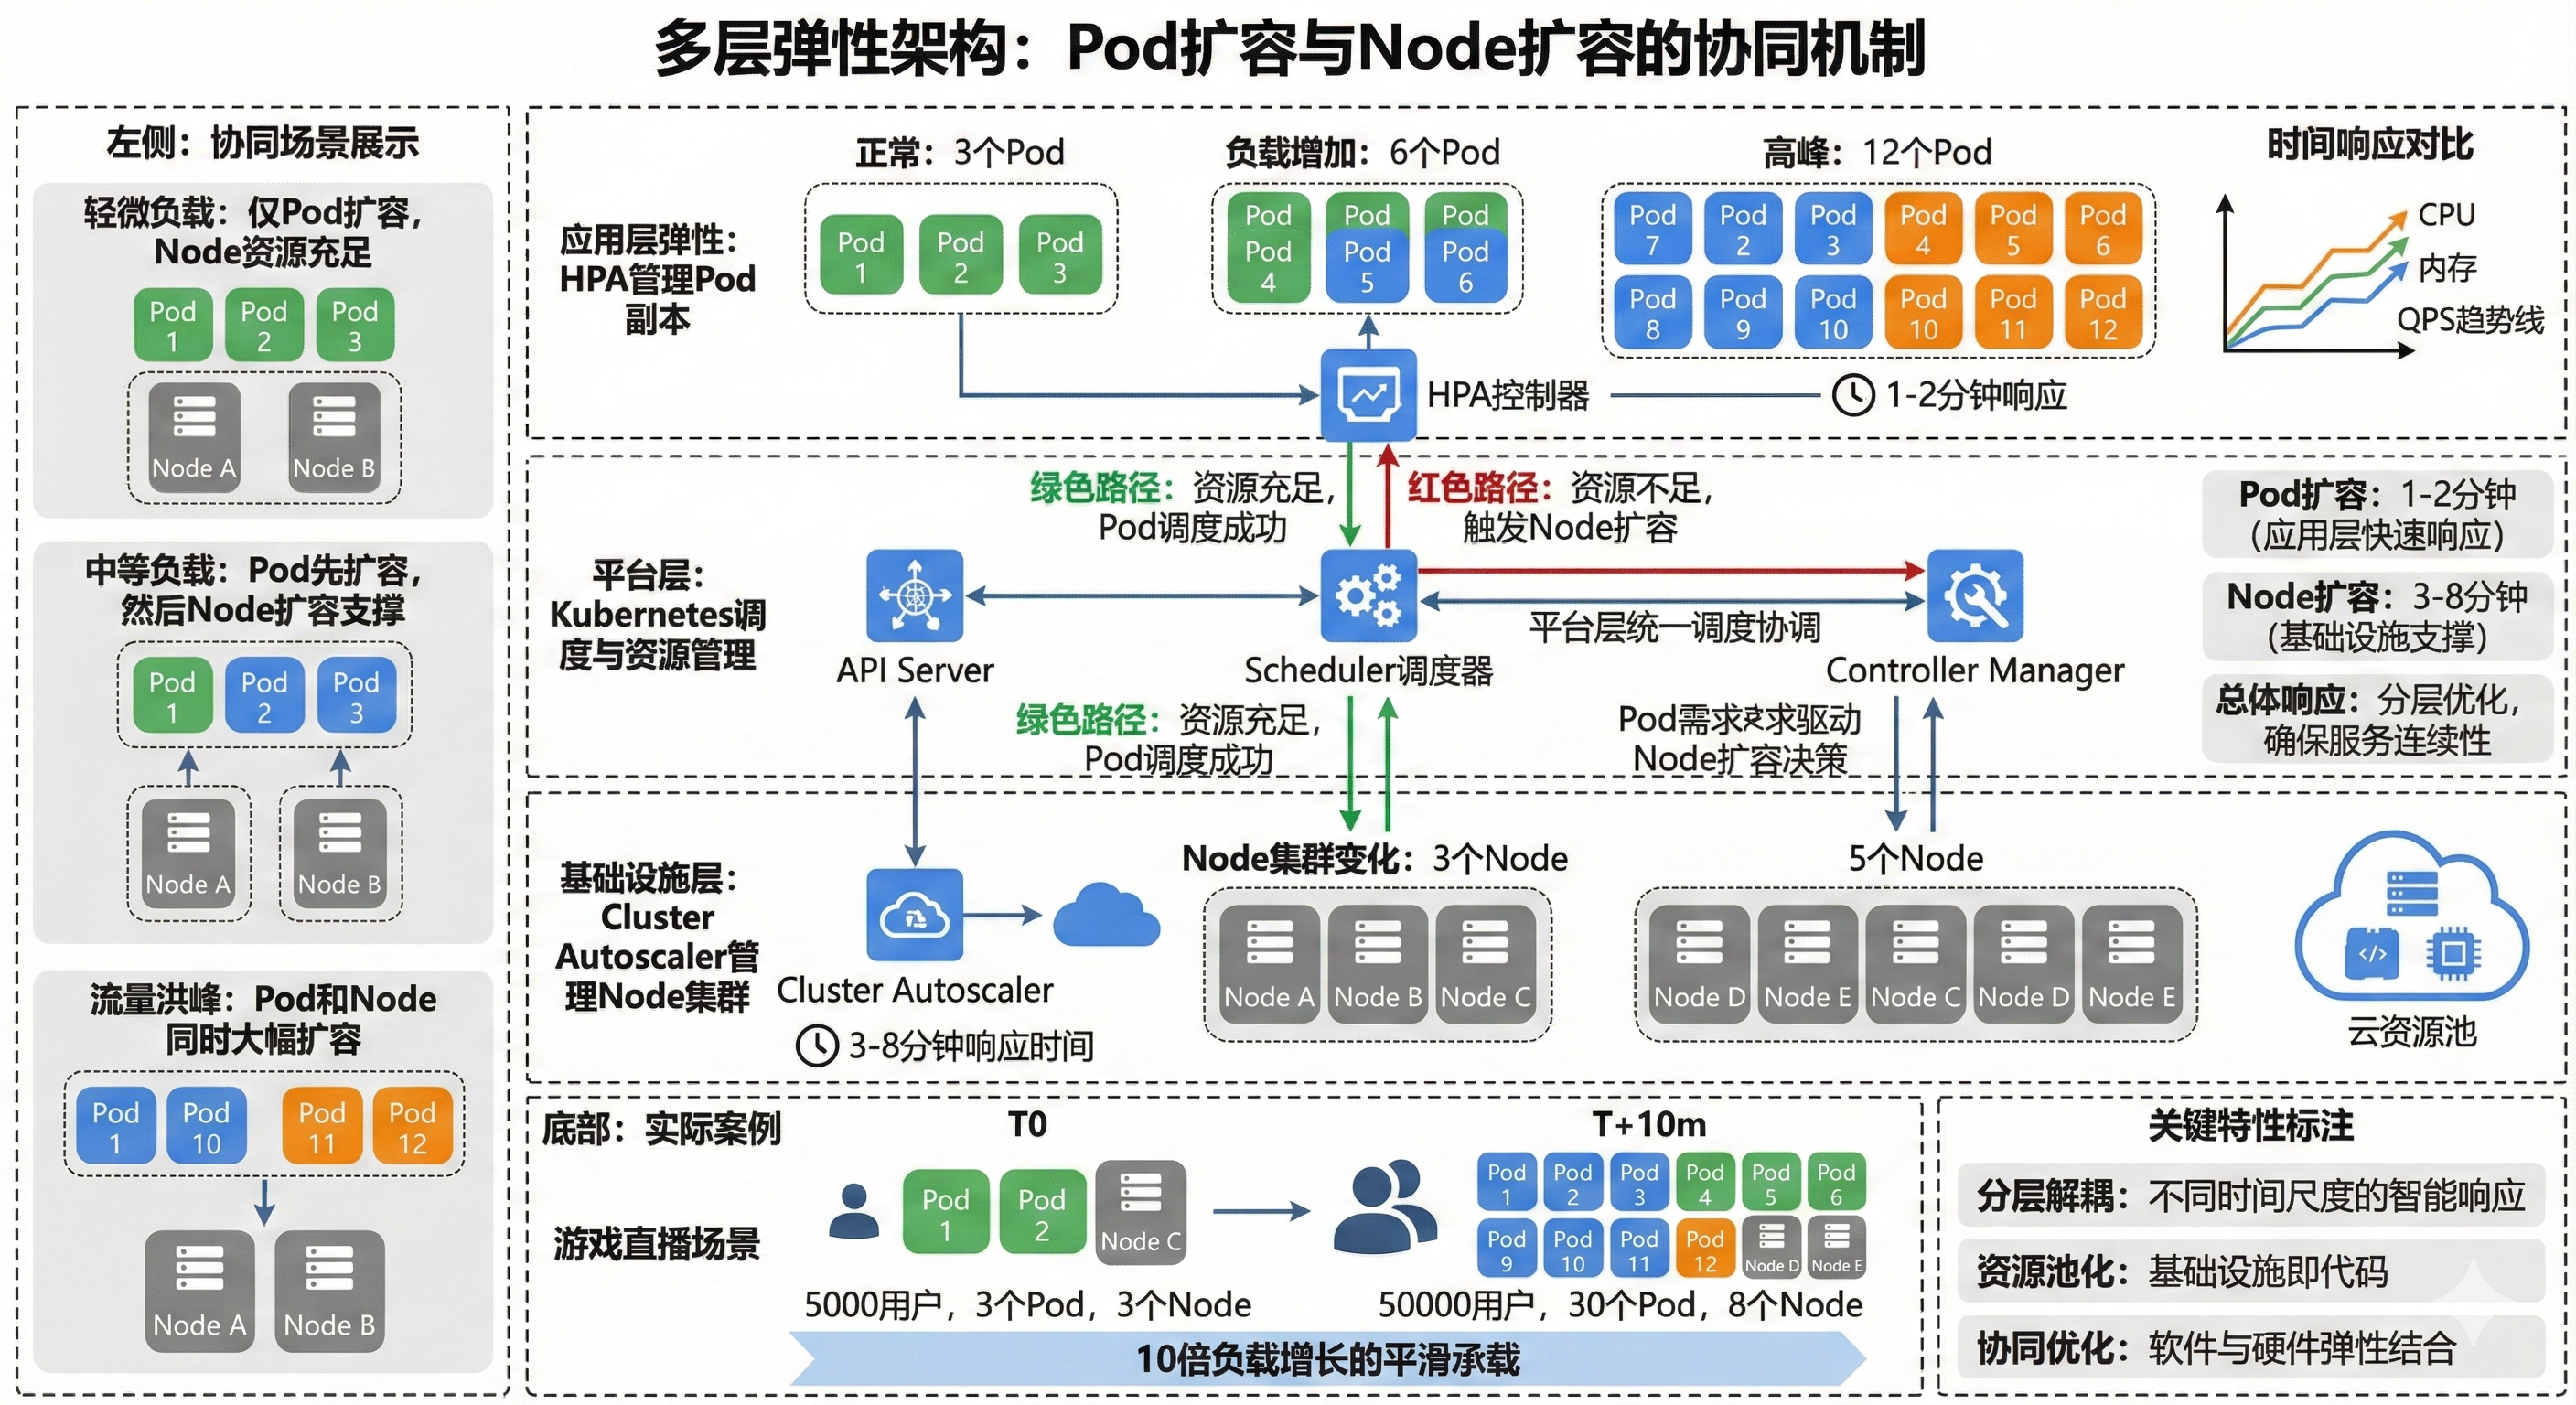
\includegraphics[width=0.9\textwidth]{figures/sec5/multi-layer-elasticity.png}
\caption{多层弹性架构：Pod扩容与Node扩容的协同机制}
\label{fig:multi-layer-elasticity}
\end{figure}

这种分层设计的优势在于它能够处理不同时间尺度和不同强度的负载变化。对于短期的负载波动，HPA能够快速响应，在现有资源范围内进行精细调节；对于长期的容量需求增长，Cluster Autoscaler提供底层支撑，确保有足够的基础资源来承载更多的Pod。两者配合，实现了从秒级到分钟级、从软件层到硬件层的全方位弹性覆盖。

在实际的游戏运营场景中，这种多层弹性的价值尤为明显。比如，某个热门主播开始直播游戏时，观众涌入导致在线人数在10分钟内从5000增长到50000。首先，HPA检测到CPU使用率急剧上升，开始在现有Node上快速增加游戏服务器Pod；当现有Node资源耗尽后，大量新Pod处于Pending状态，触发Cluster Autoscaler开始创建新Node；新Node加入集群后，Pending的Pod被调度到新Node上，整个系统平滑地承载了10倍的负载增长。

更重要的是，当直播结束、在线人数回落后，整个过程会反向进行：HPA首先减少多余的Pod，释放Node上的资源；Cluster Autoscaler发现某些Node利用率过低，开始缩容Node，将剩余Pod重新分布到更少的Node上，然后释放多余的云服务器。这个过程完全自动化，无需任何人工干预，真正实现了"来的时候自动扩，走的时候自动缩"的理想弹性状态。

弹性扩容的价值不仅体现在技术层面，更直接反映在成本结构上。传统做法往往按峰值一次性采购或长期预留服务器，为了扛住少数高峰，平时常有70\%到80\%资源闲置，资金与运维投入都被锁在低利用率资产里。云上弹性则是按使用付费，费用更贴近真实在线人数与请求量；但要做到"既省钱又稳"，关键在预留实例与按需实例的配比：预留实例通常比按需便宜30\%到60\%，代价是提前承诺容量与周期，按需实例单价更高但调度最灵活。对游戏场景，建议把稳定底座（如长期在线的5000并发）放在预留实例上，把活动冲高部分（如从5000跃升到50000并发）交给按需实例承接，这种基线预留加弹性按需的策略相较纯按需常可降低40\%到60\%总云成本。竞价实例虽然还能再便宜60\%到90\%，但可能被云厂商随时回收，适合非关键离线批处理，不应承载实时对战的在线会话链路。

通过本节的学习，我们不仅掌握了Kubernetes弹性扩容的技术机制，更重要的是理解了现代云原生架构的核心价值：将静态的资源配置转变为动态的策略管理，让系统像生物体一样具备感知环境变化并自适应调节的能力。这种弹性思维的掌握，标志着从传统运维向云原生架构师的重要转变，为构建真正具备互联网级承载能力的系统奠定了坚实基础。

当你看到监控面板上显示"Auto-scaled from 3 to 30 pods in 5 minutes"时，你就真正体验到了云原生弹性的魅力：不是简单的技术优化，而是让系统具备了应对未来不确定性的核心能力。

%\subsection{未来展望：Serverless 架构与无限可能}
%\paragraph{本节目标} 了解 Serverless 概念，掌握其应用场景。
%\paragraph{写作建议}
%\begin{enumerate}
%    \item 对比 K8s：Serverless 不用管服务器，按代码运行时间收费。
%    \item 列适用场景：低频功能（每日签到）、峰值波动功能（节日活动）、轻量逻辑（等级计算）。
%\end{enumerate}



\subsection{未来展望：Serverless架构与无限可能}

\subsubsection{从管理集群到专注业务：Serverless的范式革命}

在我们刚刚掌握的Kubernetes架构中，虽然已经实现了容器编排的自动化和弹性扩容的智能化，但仔细观察会发现，我们依然需要关心许多基础设施层面的细节：Node的规格选择、集群的健康监控、网络的安全配置、存储的持久化策略等等。这些运维工作虽然被K8s大大简化了，但并没有完全消失。对于专注业务创新的开发团队来说，这些"必要但非核心"的技术债务依然会分散精力，影响产品迭代的速度。

Serverless（无服务器）架构的出现，代表了云计算发展的下一个重要阶段：彻底抽象掉服务器管理的复杂性，让开发者只需要关心业务逻辑的实现。这种抽象程度的提升，类似于从汇编语言到高级编程语言的飞跃，或从手动内存管理到自动垃圾回收的进化。每一次抽象层次的提升，都会释放开发者的生产力，让他们能够将更多精力投入到真正创造价值的业务创新上。

在Serverless模式下，你不需要预先购买或配置任何服务器，不需要担心容器的调度和扩缩容策略，甚至不需要关心代码运行在什么操作系统上。你唯一需要做的，就是编写业务逻辑代码，然后将其部署到云厂商的Serverless平台上，平台会自动处理所有的基础设施管理工作。这种"代码即服务"的理念，让基础设施真正变成了不可见的底层支撑。

更具革命性的是，Serverless采用了全新的计费模式：按代码实际运行时间收费，而非按服务器租用时间收费。在传统模式下，即使你的游戏服务器整夜无人访问，你依然需要为那台空转的机器付费；而在Serverless模式下，如果没有玩家触发相关功能，你的代码根本不会运行，自然也不会产生任何费用。这种"用多少付多少"的精确计费，对于具有明显波峰波谷特征的业务场景来说，能够带来显著的成本优势。

\begin{figure}[htbp]
\centering
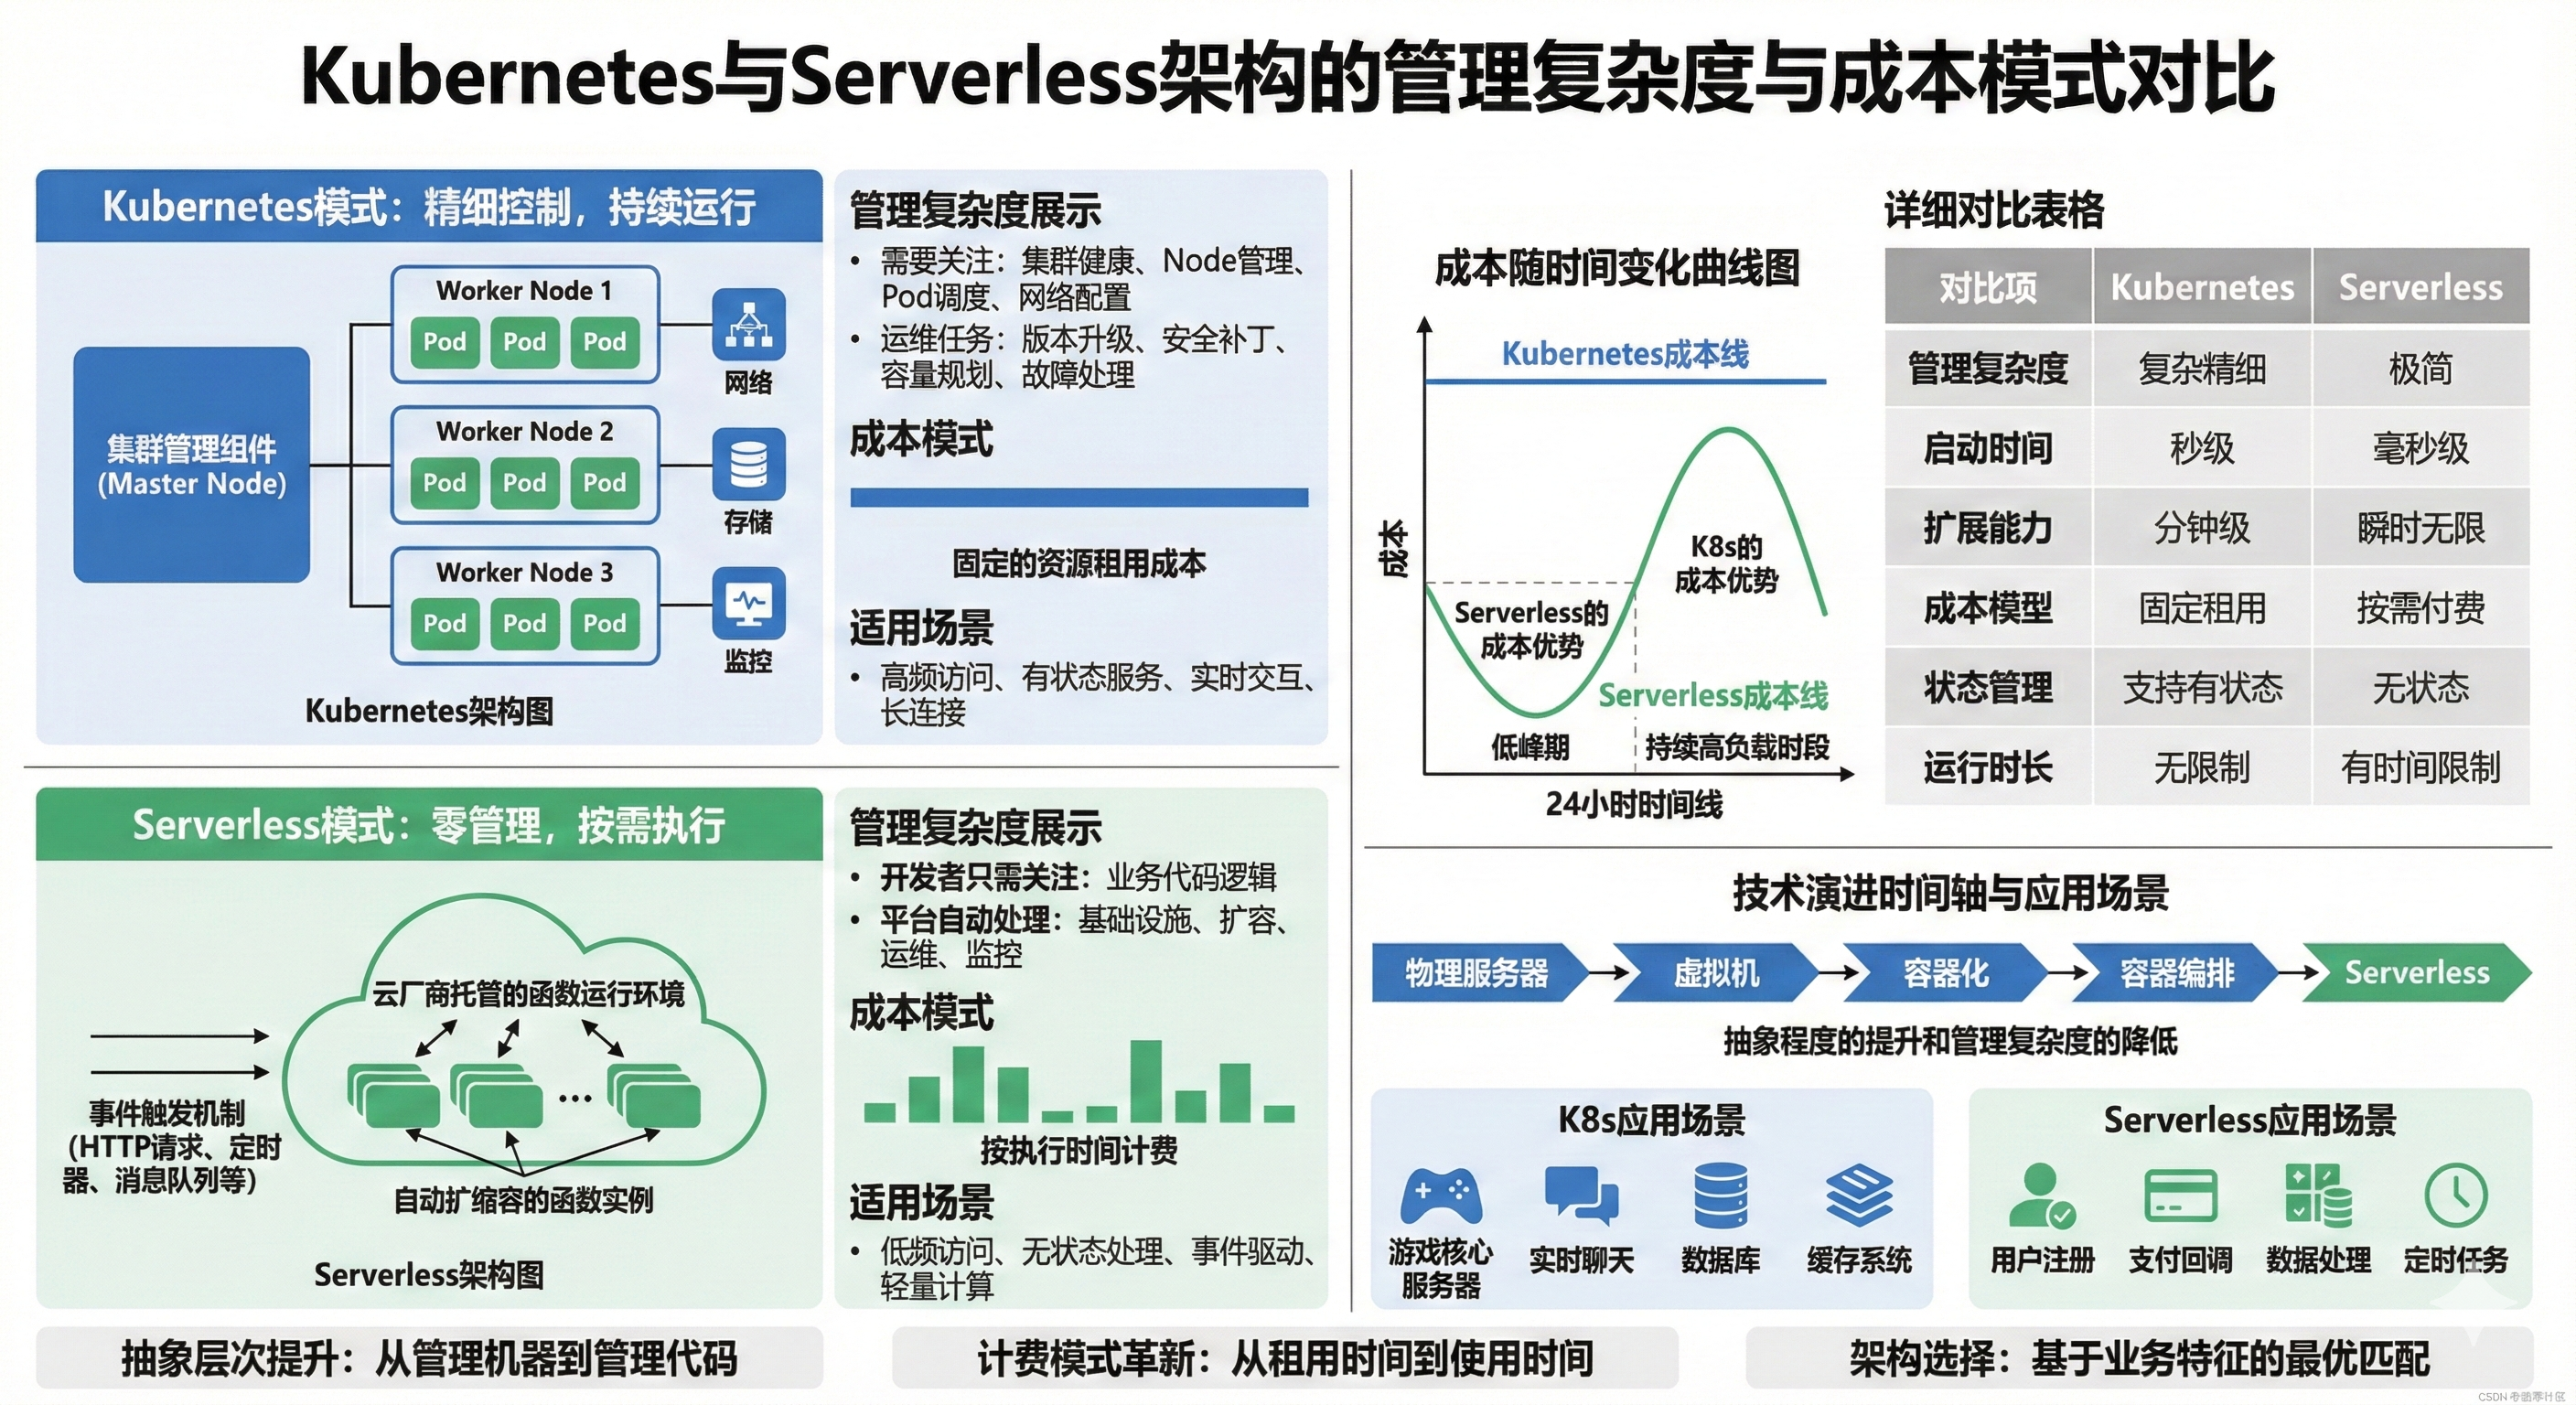
\includegraphics[width=0.9\textwidth]{figures/sec5/kubernetes-vs-serverless-comparison.png}
\caption{Kubernetes与Serverless架构的管理复杂度与成本模式对比}
\label{fig:k8s-vs-serverless}
\end{figure}

如图\ref{fig:k8s-vs-serverless}所示，两种架构模式在管理复杂度、计费方式和适用场景上存在显著差异。Kubernetes提供了更精细的控制能力和更稳定的性能表现，适合作为游戏核心服务的载体；而Serverless则以极简的管理成本和精确的按需付费，在特定业务场景下展现出独特的优势。

Serverless架构的另一个重要特征是事件驱动的执行模型。传统的服务器程序是常驻内存的，持续监听请求并做出响应；而Serverless函数是按需启动的，只在有事件触发时才会执行。这种执行模型非常适合处理不连续的业务逻辑，如用户注册、支付回调、数据同步等。当事件发生时，云平台会在毫秒级时间内启动函数实例处理请求；当处理完成后，实例立即被回收，不占用任何资源。

\subsubsection{游戏场景中的Serverless黄金应用}

虽然Serverless架构具有诸多优势，但并非适用于所有游戏业务场景。它的技术特性决定了其最适合处理低频次、突发性或轻量级的业务逻辑。通过对游戏业务特征的深入分析，我们可以识别出Serverless的几个黄金应用场景。

\textbf{低频功能的完美载体}

每日签到、邮件系统、好友申请处理等功能，虽然是游戏必备的基础模块，但其访问频率相对较低且呈现明显的时间规律性。以每日签到为例，大部分玩家会在每天的固定时间段集中签到，其余22个小时该功能几乎处于空闲状态。如果为此类功能专门维护服务器，将造成严重的资源浪费。

Serverless架构天然适合这种"间歇性高并发"的访问模式。在无人访问时，函数完全不消耗资源和费用；当出现签到高峰时，云平台能够在毫秒级时间内启动成千上万个函数实例，自动应对并发压力。更重要的是，这类功能通常不需要维持复杂的状态，单次请求可以独立处理，非常契合Serverless的无状态特性。

\textbf{突发流量的弹性缓冲器}

游戏运营中经常会遇到不可预测的突发流量：新版本发布、网红主播推荐、突发热点事件等都可能在短时间内带来数十倍的访问量增长。传统架构需要提前预估峰值并预留资源，但预估往往不准确，要么资源不足导致服务崩溃，要么过度预留造成浪费。

Serverless提供了理论上无限的并发扩展能力，能够自动应对任何规模的突发流量。当流量洪峰到来时，云平台会根据实际请求量动态启动函数实例；当流量回落时，多余的实例自动销毁。这种"用时即启动，完毕即销毁"的执行模式，让系统具备了应对"黑天鹅事件"的能力，而无需为极端情况买单。

节日活动、限时副本、抢购活动等具有明显时效性的功能，特别适合采用Serverless架构。活动期间可以获得充足的计算资源，活动结束后立即停止资源消耗，实现了真正的按需使用。

\begin{figure}[htbp]
\centering
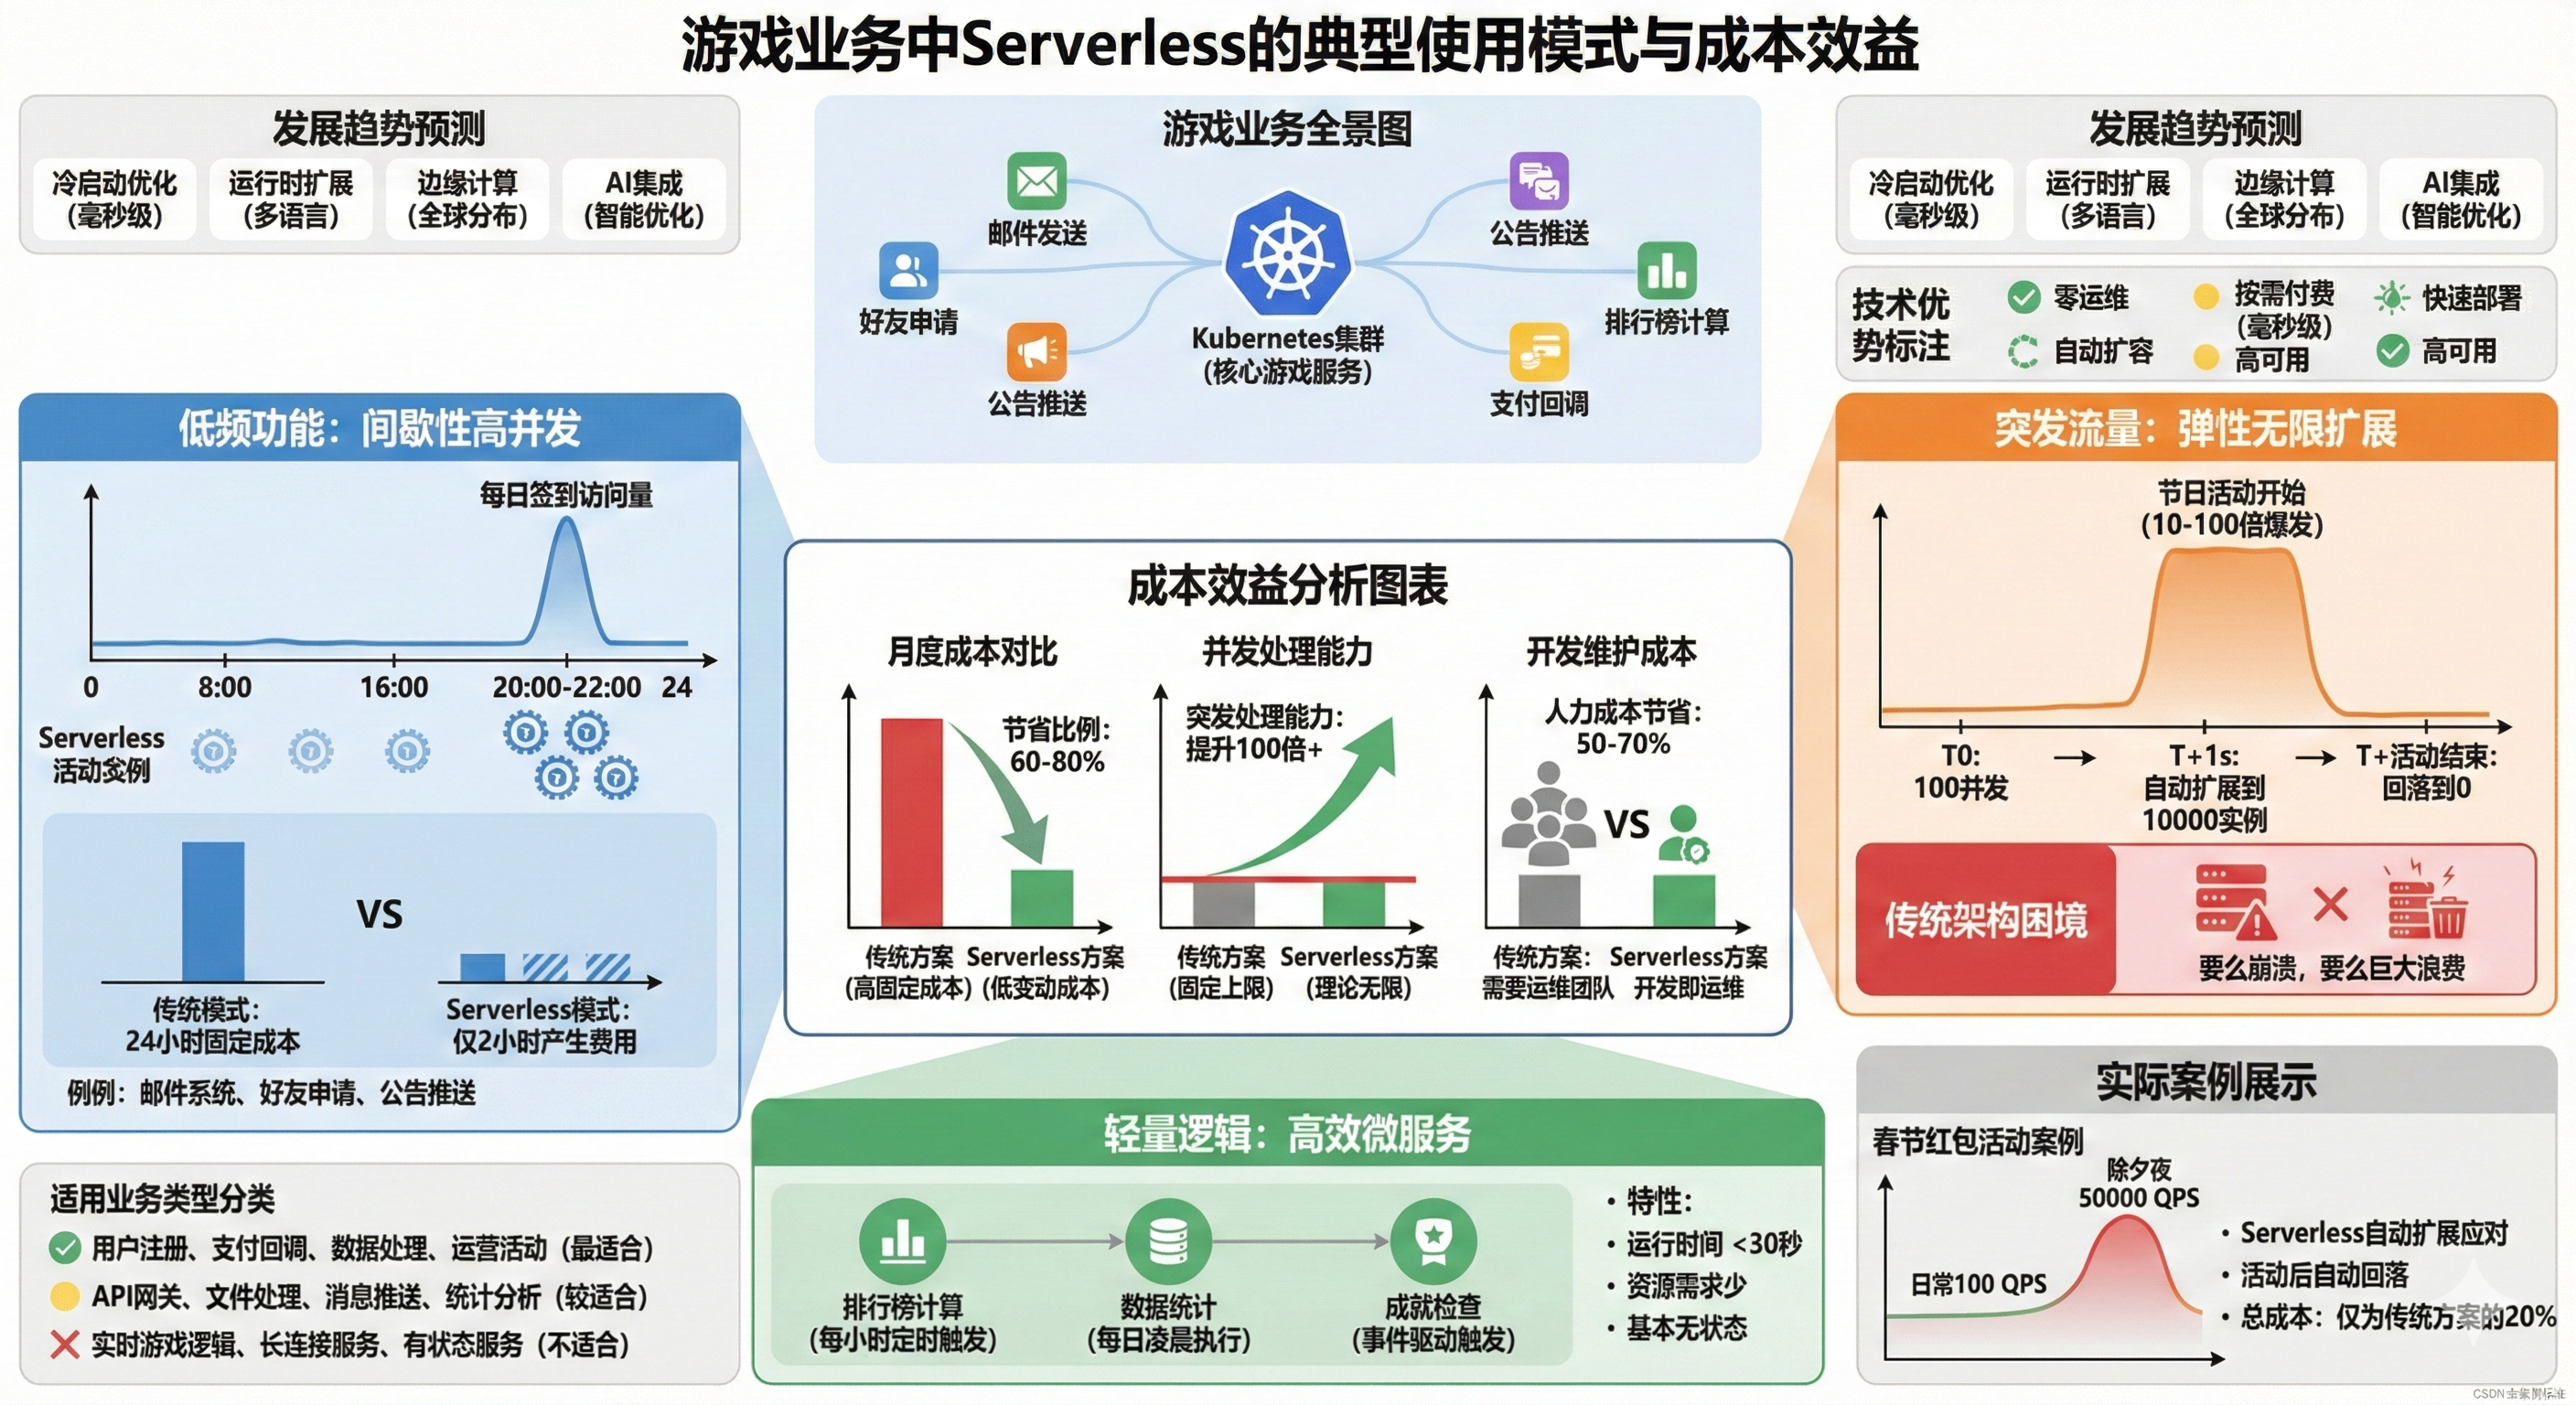
\includegraphics[width=0.9\textwidth]{figures/sec5/serverless-usage-patterns.png}
\caption{游戏业务中Serverless的典型使用模式与成本效益}
\label{fig:serverless-patterns}
\end{figure}

\textbf{轻量逻辑的高效执行器}

游戏中存在大量轻量级的计算任务：排行榜更新、成就进度检查、每日任务重置、数据统计分析等。这些任务通常逻辑简单、执行时间短暂、不需要复杂的资源管理，但又是游戏运营不可缺少的重要环节。

Serverless函数非常适合承载这类轻量级任务。函数的冷启动时间已经优化到百毫秒级别，对于大多数计算任务来说完全可以接受。但冷启动并不是一个单点事件，而是由多个串行阶段叠加形成的端到端时延。第一阶段是执行环境创建，平台需要完成沙箱分配、网络与文件系统挂载等基础准备；在主流实现中，Firecracker microVM 的启动时间大约可做到 125\,ms，同时保持接近传统虚拟机级别的隔离性。第二阶段是运行时初始化，不同语言差异显著：Go 与 Rust 的启动开销通常接近零，Python 和 Node.js 往往会增加几十到数百毫秒，而传统 JVM 在类加载和 JIT 预热场景下可能增加秒级延迟。第三阶段是应用代码加载，这部分最受开发者控制，常见耗时来自依赖导入、数据库连接建立、配置读取与客户端初始化。

工程上应把优化重点放在可控环节：对稳定高峰流量使用预留并发（Provisioned Concurrency）进行预热，但要明确这会增加常驻成本；优先选择轻量运行时；JVM 场景可考虑 GraalVM Native Image 缩短启动路径；同时缩小部署包体积、减少无关依赖，并通过延迟加载将非首请求必需逻辑后置。这样可以把冷启动从"平台黑盒问题"转化为"可测量、可分解、可治理"的性能工程问题。关于 Firecracker 的内部机制以及快照恢复（Snapshot-Restore）如何进一步压缩甚至消除冷启动，我们将在第六章展开。

而且，这类任务往往可以设计为定时触发或事件驱动，与Serverless的执行模型天然匹配。

例如，排行榜计算可以设计为每小时定时触发的Serverless函数，从数据库读取玩家数据，进行排序计算，然后将结果写入缓存。整个过程只需要几秒钟的执行时间，但如果用传统方式部署专门的服务器，就需要7×24小时运行以等待这每小时一次的任务执行。

\subsubsection{架构融合：构建最优的混合云策略}

在实际的游戏项目中，Serverless并不是要完全替代Kubernetes，而是与其形成优势互补的混合架构。这种架构选择的核心原则是：让合适的技术处理合适的场景，实现整体系统的最优性价比。

核心游戏服务（如实时对战、世界状态同步、聊天系统）需要维持长连接、处理高频交互、管理复杂状态，这类服务依然适合运行在Kubernetes集群上。K8s提供的精细资源控制、网络管理、存储编排等能力，能够保证核心服务的稳定性和性能。

而周边的辅助功能（如用户注册、支付回调、数据分析、运营活动）则可以逐步迁移到Serverless平台，实现成本优化和运维简化。这些功能通常具有无状态、低频次、可独立执行的特点，正好契合Serverless的技术优势。

\begin{figure}[htbp]
\centering
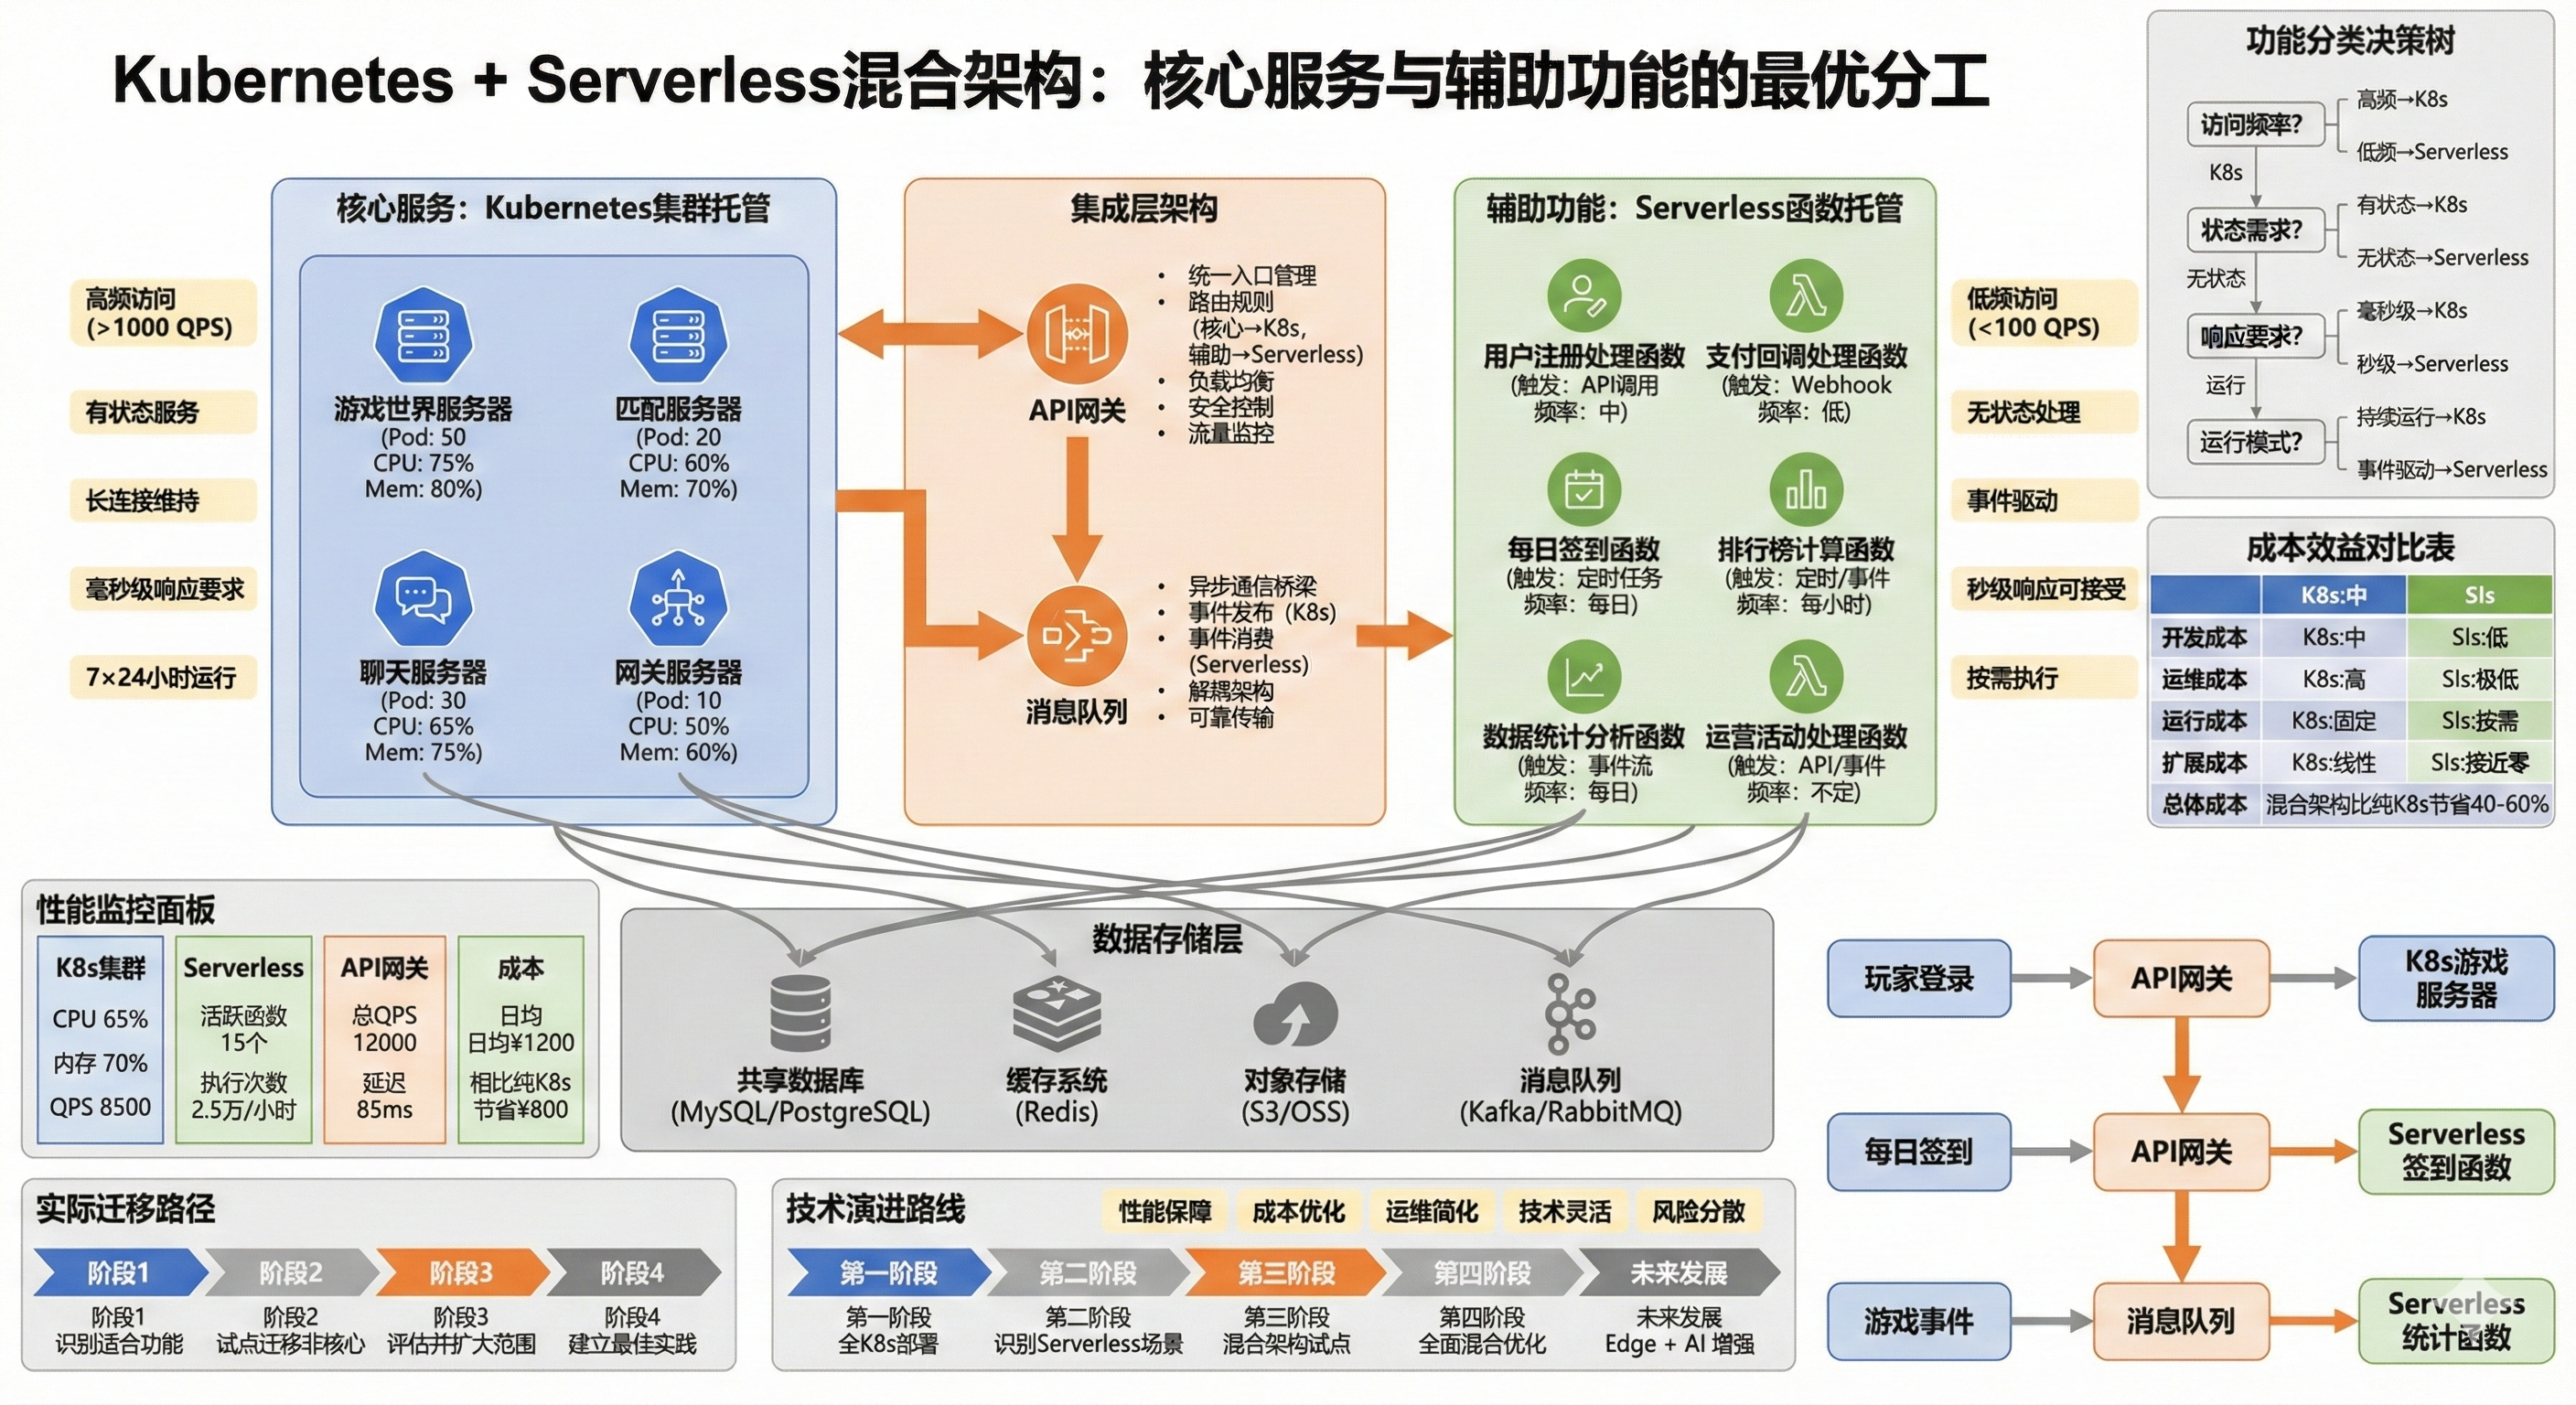
\includegraphics[width=0.9\textwidth]{figures/sec5/hybrid-architecture-design.png}
\caption{Kubernetes + Serverless混合架构：核心服务与辅助功能的最优分工}
\label{fig:hybrid-architecture}
\end{figure}

如图\ref{fig:hybrid-architecture}所示，混合架构通过合理的功能分层，既保证了游戏核心体验的稳定性，又充分利用了Serverless在成本和运维方面的优势。两种架构通过API网关、消息队列、共享数据库等方式实现无缝集成，形成统一的技术生态。

这种混合策略的实施可以采用渐进式迁移的方式：首先识别系统中适合Serverless的功能模块，评估迁移的技术可行性和商业价值；然后逐个模块进行迁移试点，积累经验和最佳实践；最后基于试点效果决定进一步的迁移范围。这种approach既能够快速获得Serverless的收益，又能够将迁移风险控制在可接受范围内。

为了把"何时选 Serverless、何时保留 K8s"从经验判断变成可执行决策，可以先按业务特征做一轮快速映射。

\begin{table}[htbp]
\centering
\caption{Serverless 与 Kubernetes 的场景化决策参考}
\label{tab:serverless-k8s-decision}
\begin{tabular}{|p{0.26\textwidth}|p{0.18\textwidth}|p{0.46\textwidth}|}
\hline
业务特征 & 推荐方案 & 主要原因 \\
\hline
长连接实时交互 & Kubernetes & WebSocket/TCP 长连接需要稳定连接驻留，容器常驻模型更匹配 \\
\hline
有状态会话管理 & Kubernetes & 会话粘性、进程内状态与低抖动路由更容易在 K8s 中实现 \\
\hline
低频触发式任务 & Serverless & 按调用计费可避免空闲资源浪费，成本可下降 90\% 以上 \\
\hline
不可预测突发流量 & Serverless & 自动弹性能力强，能快速扩缩并减少人工容量规划压力 \\
\hline
定时批处理 & Serverless & 与事件调度天然契合，任务短平快且资源利用率高 \\
\hline
延迟敏感（$<$50\,ms） & Kubernetes & 冷启动尾延迟风险较高，常驻实例更容易保障严格时延目标 \\
\hline
\end{tabular}
\end{table}

这张表是决策指引而非绝对规则。随着 KEDA、provisioned concurrency 等能力的发展，两种范式正在持续收敛并形成混合架构新常态。

\subsubsection{技术展望：Serverless的未来演进}

随着云厂商对Serverless技术的持续投入和优化，其技术能力边界正在不断扩展。冷启动时间从秒级优化到毫秒级，执行环境从简单脚本扩展到完整应用，触发方式从HTTP请求扩展到数十种事件源，运行时长从几分钟扩展到几小时。这些技术进步让Serverless能够承载越来越复杂的业务场景。

特别值得关注的是边缘计算与Serverless的结合。云厂商正在将Serverless计算能力部署到全球各地的边缘节点，让函数能够在离用户更近的位置执行。这种Edge Serverless架构对于游戏业务具有特殊意义：可以显著降低网络延迟，提升玩家体验；可以就近处理地域性的业务逻辑，减少数据传输成本；可以更好地支持全球化运营，适应不同地区的监管要求。

另一个重要的发展方向是Serverless与AI/ML的深度集成。云平台正在提供越来越多的预训练AI模型和机器学习服务，这些服务可以通过Serverless函数轻松调用。对于游戏业务来说，这意味着可以用极低的成本构建智能化功能：智能客服、内容审核、个性化推荐、作弊检测等，而无需投入大量资源来构建和维护AI基础设施。

可以预见，未来一个理想的游戏后端架构将是这样的：Kubernetes集群承载核心的游戏世界，提供稳定的实时交互能力；Serverless函数处理所有的辅助功能，提供极致的成本效率；Edge Computing将部分逻辑推送到用户附近，提供最优的响应体验；AI Services提供智能化的增值功能，提升产品竞争力。这四大技术栈相互协作，共同构建一个既高性能又低成本、既稳定可靠又灵活敏捷的云原生游戏生态。

进入第六章后，我们会从底层机制解释这种收敛：为什么 Firecracker microVM 能把沙箱创建压缩到 200\,ms 以内，为什么 snapshot-restore 正在让冷启动趋近可忽略，以及有状态 Serverless 如何逐步打破"容器负责状态、函数只做无状态"的旧边界。这些看似底层的机制，正是支撑云原生游戏生态演进的"屠龙之术"。

通过本章的学习，我们完成了从本地开发到云端部署的完整技术栈掌握：Docker容器化解决了环境一致性问题，Kubernetes提供了工业级的编排能力，弹性扩容实现了资源的智能调度，而Serverless则为特定场景提供了更优的解决方案。这套完整的云原生技术体系，将为你构建下一代游戏产品提供坚实的技术底座。

当你能够灵活运用这些技术，根据业务特点选择最适合的架构模式时，你就真正掌握了云原生时代的核心竞争力：不是简单地使用某种技术，而是基于深度理解来设计最优的技术组合，让技术真正服务于业务价值的创造。


% \subsubsection{小结：从“本地原型”到“云原生工业”}

% 本章的旅程，实质上是一场对软件交付模式的工业化革命。在章节之初，我们还困在“本地原型”的局限中，依赖开发者的个人电脑和手工配置，像呵护盆栽一样小心翼翼地维护着单体服务。而通过引入 Docker，我们首先解决了“标准化零件”的问题，让代码与其运行环境彻底解耦，实现了“一次构建，处处运行”的交付契约。

% 随后，我们通过 Kubernetes 建立了一套自动化的“生产流水线”。在这个阶段，我们不再关注单台服务器的死活，而是站在“集群指挥官”的视角，用声明式的配置驾驭成百上千的容器实例。我们将资源的调度权交给了算法，将故障的修复权交给了系统，让游戏世界具备了自我修复和自我进化的能力。

% 最后，通过弹性伸缩与 Serverless 的探索，我们触碰到了云原生的终极形态：让算力像水电一样“即开即用”。至此，我们的游戏架构彻底摆脱了物理硬件的重力束缚，从一个脆弱的本地原型，进化为一座能够根据流量潮汐自由呼吸、永续运行的“云原生工业堡垒”。

% 这不仅是技术概念的层层递进式学习，更是系统工程思维维度的跃升。当我们将基础设施代码化、自动化之后，我们终于可以从繁琐的运维泥潭中抽身，将精力回归到最本质的创造，为玩家编织更宏大的游戏世界。

\subsection{小结：本地到云端}
本章系统梳理了如何将游戏后端从本地环境平滑迁移至云端，实现云原生架构的关键技术路径和思维转变。我们首先解决了长期困扰开发者的“环境地狱”难题，通过 Docker 容器化技术，将应用与运行环境彻底解耦，从而实现“一次构建，处处运行”的交付保证。镜像与容器的分层机制、命名空间隔离和资源控制让我们得以实现轻量、高效且可靠的应用封装。

继而，我们引入 Docker Compose，帮助管理和协调多容器服务的集群启动，使复杂多服务系统的部署变得标准化且易于维护。Compose 的声明式配置和自动网络创建极大降低了多服务协作的运维门槛，为中小规模应用提供了理想的编排解决方案。

随着业务规模和复杂度提升，单机部署面临管理瓶颈，Kubernetes 应运而生，成为强大的分布式容器编排平台。其以声明式理念为核心，通过智能调度、服务发现、自动扩容与容错，实现了大规模集群的自动化管理。我们从核心概念到典型部署实践，深入解析了 K8s 如何成为云端“超级管家”，极大提升系统的弹性、可靠性与运维效率。
本章还着力讲解了弹性扩容的工程智慧，说明了“像呼吸一样自适应”的资源动态调整机制。通过 Pod 级别的 Horizontal Pod Autoscaler 以及 Node 级别的 Cluster Autoscaler 协同工作，实现了云资源的高效利用和业务负载的实时响应，为游戏服务应对流量波峰波谷提供坚实保障。

最后，我们展望了 Serverless 架构这一云计算前沿趋势，借助无服务器弹性计算，让开发者摆脱基建运维束缚，专注业务创新。通过合理的混合云架构组合，Kubernetes 与 Serverless 互为补充，实现游戏核心服务的稳定运行与周边功能的成本优化，为下一代云原生游戏构建最优技术栈。
综上所述，本章不仅提供了从“本地原型”到“云原生工业”的技术路线图，更引导读者跨越环境、规模、自动化和弹性四大关键壁垒。掌握这些关键技术与理念，将使你在构建下一代高性能、可扩展、可靠的云端游戏服务时游刃有余，真正迈入工业化云原生时代的大门。

\newpage